%----------
%   WARNING
%----------

% This Guide contains Library recommendations based mainly on APA and IEEE styles, but you must always follow the guidelines of your TFG Tutor and the TFG regulations for your degree.

% THIS TEMPLATE IS BASED ON THE IEEE STYLE 


%----------
% DOCUMENT SETTINGS
%----------

\documentclass[12pt]{report} % font: 12pt

% Custom packages
\usepackage{comment}
\usepackage[numbers]{natbib}
\usepackage{booktabs}
\usepackage[table,xcdraw]{xcolor}
\usepackage[normalem]{ulem}
\usepackage{amsmath}
\usepackage{subcaption}

\useunder{\uline}{\ul}{}

\bibliographystyle{IEEEtran}


% margins: 2.5 cm top and bottom; 3 cm left and right
\usepackage[
a4paper,
vmargin=2.5cm,
hmargin=3cm
]{geometry}

% Paragraph Spacing and Line Spacing: Narrow (6 pt / 1.15 spacing) or Moderate (6 pt / 1.5 spacing)
\renewcommand{\baselinestretch}{1.15}
\parskip=6pt

% Color settings for cover and code listings 
\usepackage[table]{xcolor}
\definecolor{azulUC3M}{RGB}{0,0,102}
\definecolor{gray97}{gray}{.97}
\definecolor{gray75}{gray}{.75}
\definecolor{gray45}{gray}{.45}

% PDF/A -- Important for its inclusion in e-Archive. PDF/A is the optimal format for preservation and for the generation of metadata: http://uc3m.libguides.com/ld.php?content_id=31389625. 

% In the template we include the file OUTPUT.XMPDATA. You can download that file and include the metadata that will be incorporated into the PDF file when you compile the memoria.tex file. Then upload it back to your project.  
\usepackage[a-1b]{pdfx}

% LINKS
\usepackage{hyperref}
\hypersetup{colorlinks=true,
	linkcolor=black, % links to parts of the document (e.g. index) in black
	urlcolor=blue} % links to resources outside the document in blue

% MATH EXPRESSIONS
\usepackage{amsmath,amssymb,amsfonts,amsthm}

% Character encoding
\usepackage{txfonts} 
\usepackage[T1]{fontenc}
\usepackage[utf8]{inputenc}

% English settings
\usepackage[english]{babel} 
\usepackage[babel, english=american]{csquotes}
\AtBeginEnvironment{quote}{\small}

% Footer settings
\usepackage{fancyhdr}
\pagestyle{fancy}
\fancyhf{}
\fancyhead[R]{\MakeUppercase{6007ENG - Industry Affiliates Program, Trimester 1, 2023}}
\fancyfoot[R]{Jessy Barber - Griffith University | \thepage}
\fancypagestyle{plain}{\pagestyle{fancy}}
\renewcommand{\headrulewidth}{0pt}

% DESIGN OF THE TITLES of the parts of the work (chapters and epigraphs or sub-chapters)
\usepackage{titlesec}
\usepackage{titletoc}
\titleformat{\chapter}[block]
{\large\bfseries\filcenter}
{\thechapter.}
{5pt}
{\MakeUppercase}
{}
\titlespacing{\chapter}{0pt}{0pt}{*3}
\titlecontents{chapter}
[0pt]                                               
{}
{\contentsmargin{0pt}\thecontentslabel.\enspace\uppercase}
{\contentsmargin{0pt}\uppercase}                        
{\titlerule*[.7pc]{.}\contentspage}                 

\titleformat{\section}
{\bfseries}
{\thesection.}
{5pt}
{}
\titlecontents{section}
[5pt]                                               
{}
{\contentsmargin{0pt}\thecontentslabel.\enspace}
{\contentsmargin{0pt}}
{\titlerule*[.7pc]{.}\contentspage}

\titleformat{\subsection}
{\normalsize\bfseries}
{\thesubsection.}
{5pt}
{}
\titlecontents{subsection}
[10pt]                                               
{}
{\contentsmargin{0pt}                          
	\thecontentslabel.\enspace}
{\contentsmargin{0pt}}                        
{\titlerule*[.7pc]{.}\contentspage}  


% Tables and figures settings
\usepackage{multirow} % combine cells 
\usepackage{caption} % customize the title of tables and figures
\usepackage{floatrow} % we use this package and its \ ttabbox and \ ffigbox macros to align the table and figure names according to the defined style.
\usepackage{array} % with this package we can define in the following line a new type of column for tables: custom width and centered content
\newcolumntype{P}[1]{>{\centering\arraybackslash}p{#1}}
\DeclareCaptionFormat{upper}{#1#2\uppercase{#3}\par}
\usepackage{graphicx}
\graphicspath{{imagenes/}} % Images folder

% Table layout for engineering
\captionsetup*[table]{
	format=upper,
	name=TABLE,
	justification=centering,
	labelsep=period,
	width=.75\linewidth,
	labelfont=small,
	font=small
}

% Figures layout for engineering
\captionsetup[figure]{
	format=hang,
	name=Fig.,
	singlelinecheck=off,
	labelsep=period,
	labelfont=small,
	font=small		
}

% FOOTNOTES
\usepackage{chngcntr} % continuous numbering of footnotes
\counterwithout{footnote}{chapter}

% CODE LISTINGS 
% support and styling for listings. More information in  https://es.wikibooks.org/wiki/Manual_de_LaTeX/Listados_de_código/Listados_con_listings
\usepackage{listings}

% Custom listing
\lstdefinestyle{estilo}{ frame=Ltb,
	framerule=0pt,
	aboveskip=0.5cm,
	framextopmargin=3pt,
	framexbottommargin=3pt,
	framexleftmargin=0.4cm,
	framesep=0pt,
	rulesep=.4pt,
	backgroundcolor=\color{gray97},
	rulesepcolor=\color{black},
	%
	basicstyle=\ttfamily\footnotesize,
	keywordstyle=\bfseries,
	stringstyle=\ttfamily,
	showstringspaces = false,
	commentstyle=\color{gray45},     
	%
	numbers=left,
	numbersep=15pt,
	numberstyle=\tiny,
	numberfirstline = false,
	breaklines=true,
	xleftmargin=\parindent
}

\captionsetup*[lstlisting]{font=small, labelsep=period}
 
\lstset{style=estilo}
\renewcommand{\lstlistingname}{\uppercase{Código}}


% REFERENCES 

% IEEE bibliography setup
\begin{comment}
\usepackage[backend=biber, style=ieee, isbn=false,sortcites, maxbibnames=6, minbibnames=1]{biblatex} % Setting for IEEE citation style, recommended for engineering. "maxbibnames" indicates that from 6 authors truncate the list in the first one (minbibnames) and add "et al." as used in the IEEE style.

\addbibresource{Sections/Bibliography/References.bib} % The references.bib file in which the bibliography used should be
\end{comment}

%-------------
%	DOCUMENT
%-------------

\begin{document}
\pagenumbering{roman} % Roman numerals are used in the numbering of the pages preceding the body of the work.
	
%----------
%	COVER
%----------	

\begin{titlepage}
	\begin{sffamily}
	\color{azulUC3M}
	\begin{center}
		\begin{comment}
		\begin{figure}[H] % UC3M Logo
			\makebox[\textwidth][c]{\includegraphics[width=16cm]{logo_UC3M.png}}
		\end{figure}
		\end{comment}
		\vspace{2.5cm}
		\begin{Large}
			Bachelor of Electrical and Electronic Engineering (Honours)\\			
			 2023\\ % Academic year
			\vspace{2cm}		
			\textsl{6007ENG - Industry Affiliates Program}
			\bigskip
			
		\end{Large}
		 	{\Huge Structural Health Monitoring of the Griffith Footbridge Using LoRaWAN Technology}\\
		 	\vspace*{0.5cm}
	 		\rule{10.5cm}{0.1mm}\\
			\vspace*{0.9cm}
			{\LARGE Jessy Barber}\\ 
			\vspace*{1cm}
		\begin{Large}
			Griffith University Internal Project\\
			Yong Zhu
		\end{Large}
	\end{center}
	\vfill
	\begin{figure}
		
\includegraphics{griffithlogo.png}
	\end{figure}
	\end{sffamily}
\end{titlepage}


%----------
%	ABSTRACT AND KEYWORDS 
%----------	
\renewcommand\abstractname{\large\bfseries\filcenter\uppercase{Executive Summary}}
\begin{abstract}
\thispagestyle{plain}
\setcounter{page}{1}
	
	% Write your abstract
This research presents a novel approach for Structural Health Monitoring (SHM) of the Griffith University footbridge, harnessing the power of LoRaWAN technology within the framework of the Internet of Things (IoT). The study is undertaken in two phases. 
	
The first phase focuses on the software development and testing of the initial three layers of the IoT architecture: coding, perception and network. This involves the utilisation of two Arduino MKRWAN 1300 devices, where one serves as a LoRa node and the other as a LoRaWAN gateway. An ADXL335 3-axis accelerometer is integrated into the system to capture vibrational data, which is processed and visualized through Python scripts. 
	
The second phase extends the reach of the IoT architecture to incorporate middleware and application layers. It also includes hardware modifications like transitioning to a custom PCB and a 3D printed enclosure. The data captured is transmitted via a LoRaWAN connection to a WisGate Edge Lite 2 gateway and then relayed to the TNN cloud. Data visualization and analysis are facilitated using the Arduino IoT Cloud dashboard.
	
Each phase is guided by defined objectives, including hardware design and testing, software validation, and comprehensive field tests. The overall outcome is a potential new standard for bridge health monitoring using LoRaWAN technology, as exemplified by the Griffith University footbridge.
	
	\vfill
\end{abstract}



%----------
%	Dedication
%----------	
\chapter*{Acknowledgements}

\setcounter{page}{2}
	
	% Write here	
	I would like this opportunity to acknowledge and thank the following people, without whom I would not be able to complete this project:

My mother and father, for always supporting me every step of the way on my academic journey. For supporting me both mentally and financially during my studies, I thank you deeply. 

My group of friends, for respecting the time required for my studies, and always being there to elevate my spirits. 

My fellow peers at Griffith who I have met along the way, I thank you for being patient with me and always providing a fun learning experience. 

My work staff and bosses, for allowing me to take time off from my dream job to complete my degree, and allowing me to come back full time the moment I finish. 

And finally I would like to thank my supervisor Yong Zhu and project partner Huiyue Qiao for their countless hours in meetings and extensive laboratory testing. I hope you enjoyed the project as much as I did. 
	\vfill

	

%----------
%	TOC
%----------	

%--
% TOC
%-
\tableofcontents
\thispagestyle{fancy}


%--
% List of figures. If they are not included, comment the following lines
%-
\listoffigures
\thispagestyle{fancy}


%--
% List of tables. If they are not included, comment the following lines
%-
\listoftables
\thispagestyle{fancy}


%----------
%	THESIS
%----------	
\clearpage
\pagenumbering{arabic} % numbering with Arabic numerals for the rest of the document.	
\pagestyle{fancy}
\chapter{Introduction}
\section{Report Structure}

The report is organized in the following structure; first relevant background information regarding measuring the health of a bridge, WSNs, LoRa and LoRawan, and the internet of things will be presented. Following this, the aims and objectives of this report will be outlined. Next, a review of the relevant published literature will be evaluated. The design specifications and methodology for developing protoype one and two will be provided. Results from testing both prototype implementations will be presented and a discussion regarding these results and performance will be provided. Device limitations will be analysed, suggestions for further improvements will be discussed followed by a conclusion. Proceeding the conclusion will be the references and appendices. 
\section{Project Background}

\subsection{Wireless Sensor Networks}
Wireless Sensor Networks (WSNs) are simple, low-cost networks that primarily consist of nodes and a base station \cite{WSN-WaterQual}. WSN nodes usually comprise of some sensing or measuring capability acting as the physical layer, and relay this information via uplink to a base station for processing and then to a network server acting as the network layer. From here, the API from a network cloud service can be used to create GUI's and other applications for researchers and consumers which acts as the application layer. 

Innovating many field of industry and research, these distributed networks of nodes have been valuable in many contexts. For example, the use of ZigBee communication technology for air pollution monitoring \cite{ZigBeeAirPolution} and the use of Bluetooth for communication between end-devices measuring temperature, luminance, carbon dioxide and humidity for energy-saving establishments \cite{BTenergySaving}. Although these WSNs have worked in the past, the future of this technology lies in developing systems that have high scalability and range, something that ZigBee and Bluetooth inherently lack. Cellular and satellite technology are alternate approaches that offer extremely high data rates and range, however these technologies are not practical to implement in most situations due to exceedingly high costs. 

\subsection{Structural Health Monitoring}
Structural Health Monitoring (SHM) is a vital practice for ensuring the safety and longevity of civil and industrial structures \cite{SHM-IoT-Magazine}. SHM involves continuously tracking change in structures which can be attributed to material aging, environmental influences or unforeseen incidents such as traffic accidents or natural disasters. These changes can be tracked using WSNs equipped with appropriate sensor modules, and integrating data transmission capabilities. A survey investigating the implementation of IoT technology for structural health monitoring (SHM) determined that WSN technology has revolutionized the health monitoring in various fields including civil engineering \cite{SHM-IoT-Survey}. WSN  systems can be deployed to measures a vast array of SHM indicators including temperature, velocity, acceleration, frequency and displacement. WSN can be deployed on a structure such as a bridge operating as Internet of Things (IoT) nodes. This deployment highlights the advantage of using WSNs for SHM since the collected data can be uploaded to the cloud for processing and distribution. Within the context of bridge monitoring, the integration of WSN with IoT for SHM can serve various application requirements for real-time data uplink such as monitoring acceleration and frequency characteristics. This data can be plotted on a continuous time spectrum and compared to observational data such as pedestrian load to verify the validity of  simulated truss analysis models and finite elements (FE) simulation. 

\subsection{Internet of Things}
The Internet of Things (IoT) is an `interconnected network of things' \cite{IoT}, where `things' in this context is defined as an end-device with WSN type capability. The IoT architecture comprises of six-layers, the coding layer, perception layer, network layer, middle-ware layer, application layer and business layer \cite{IoT}. Thus to create this IoT architecture for research purposes the first five layers need to be implemented. LoRa end-devices act as the physical layer encompassing the coding and perception layer. The coding layer involves associating unique ID specifiers to each end device \cite{IoT} and the perception layer is involved with on-board sensing and data acquisition. The network layer is a relay of this perceptual information to a gateway, and the middle-ware layer is the IoT cloud platform that facilitates these connections and receives information from the network layer. The application layer involves pulling the API or information from the network layer and developing apps or graphical user interfaces (GUIs) to display the data.\\\\
The Things Network (TNN) is an open-source LoRaWAN network server used to construct IoT cloud applications with end-to-end encryption and secure communication \cite{LoRaWAN-Smart-Infrastructure-Monitoring}. TNN exists on the middle-ware layer and can be used to deploy an IoT architecture using LoRa end-devices in the coding and perception layer, and utilize the LoRaWAN communication protocol in the network layer. TNN offers a console and API to develop applications that serve as the architecture's application layer. Figure \ref{LoRa-IOT-Example} displays an example of an IoT architecture using WSN nodes, a LoRaWAN gateway, cloud storage and user devices. 

\begin{figure}[h]
	\centering
	\caption{The LoRa network architecture for agriculture area. \cite{LoRaWAN-WSN-Agricultual-Application}}
	\label{LoRa-IOT-Example}
	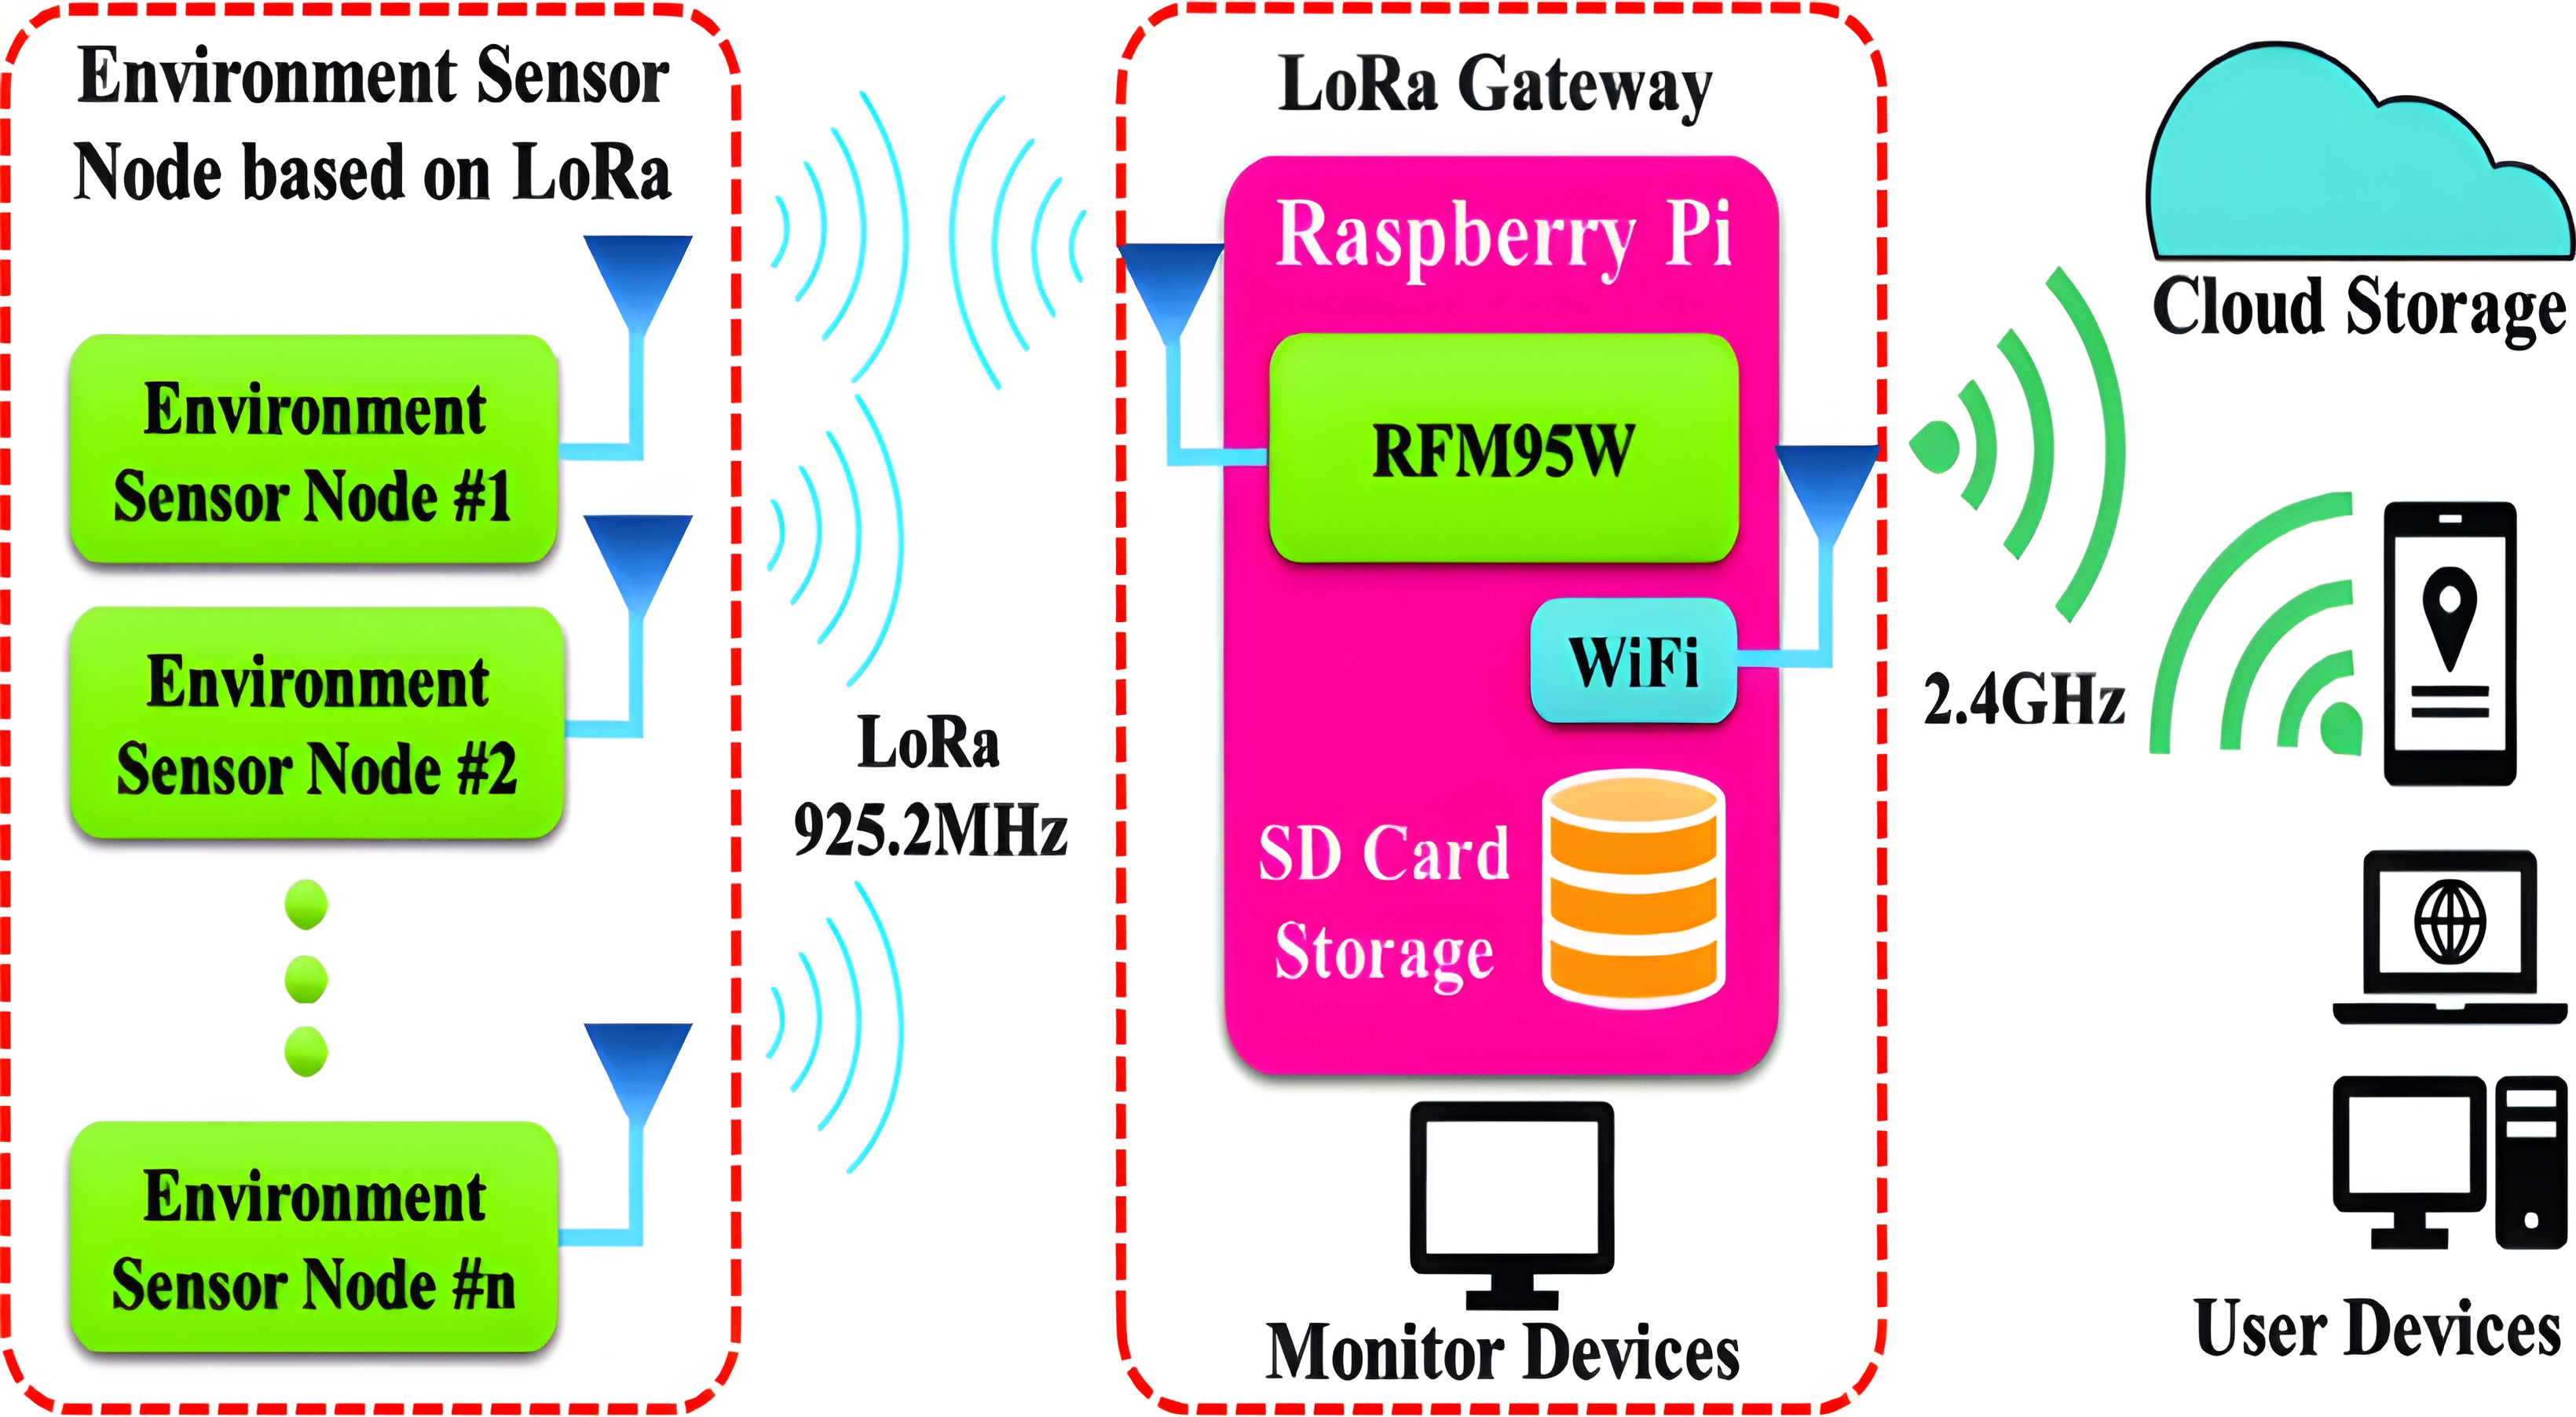
\includegraphics[scale=0.1]{Sections/Introduction/LoRaWAN-IOT-Example.jpg}
\end{figure}


\subsection{LoRa and LoRaWAN}
Low Power Wide Area Network (LPWAN) is a communication technology that offers wide coverage, similar to satellite networks, while maintaining lower data rates akin to ZigBee. The technology is distinguished by its ultra-low power consumption and cost-effective deployment and maintenance  \cite{IOTandLORAWAN-SmartFarm}.\\\\
LoRa and LoRaWAN, forms of LPWAN technology, were developed to overcome the scalabilty issues associated with traditional WSN configurations that relied on short-range communication protocols such as Zigbee and Bluetooth \cite{WSN-WaterQual}. These configurations often used a mesh network layout, which introduced challenges in network management and power consumption with increasing network size \cite{IOTandLORAWAN-SmartFarm}.\\\\
LoRaWAN's unique `star of stars' configuration addresses these challenges by enabling scalable network expansion with reduced complexity. LoRa itself is a Chirp Spread Spectrum (CSS) modulation technique developed by Cycleo, offering a Medium Access Control (MAC) protocol and operating on license-free, region-dependent Industrial, Scientific and Medical (ISM) frequency bands \cite{IOTandLORAWAN-SmartFarm}.

\begin{comment}
\begin{figure}[h]
	\centering 
	\caption{Comparison of main IoT enabling communication technologies in terms of range, data rate, energy consumption, and costs. \cite{IOTandLORAWAN-SmartFarm}}
	\label{IOTandLORAWAN-SmartFarm-Figure1}
	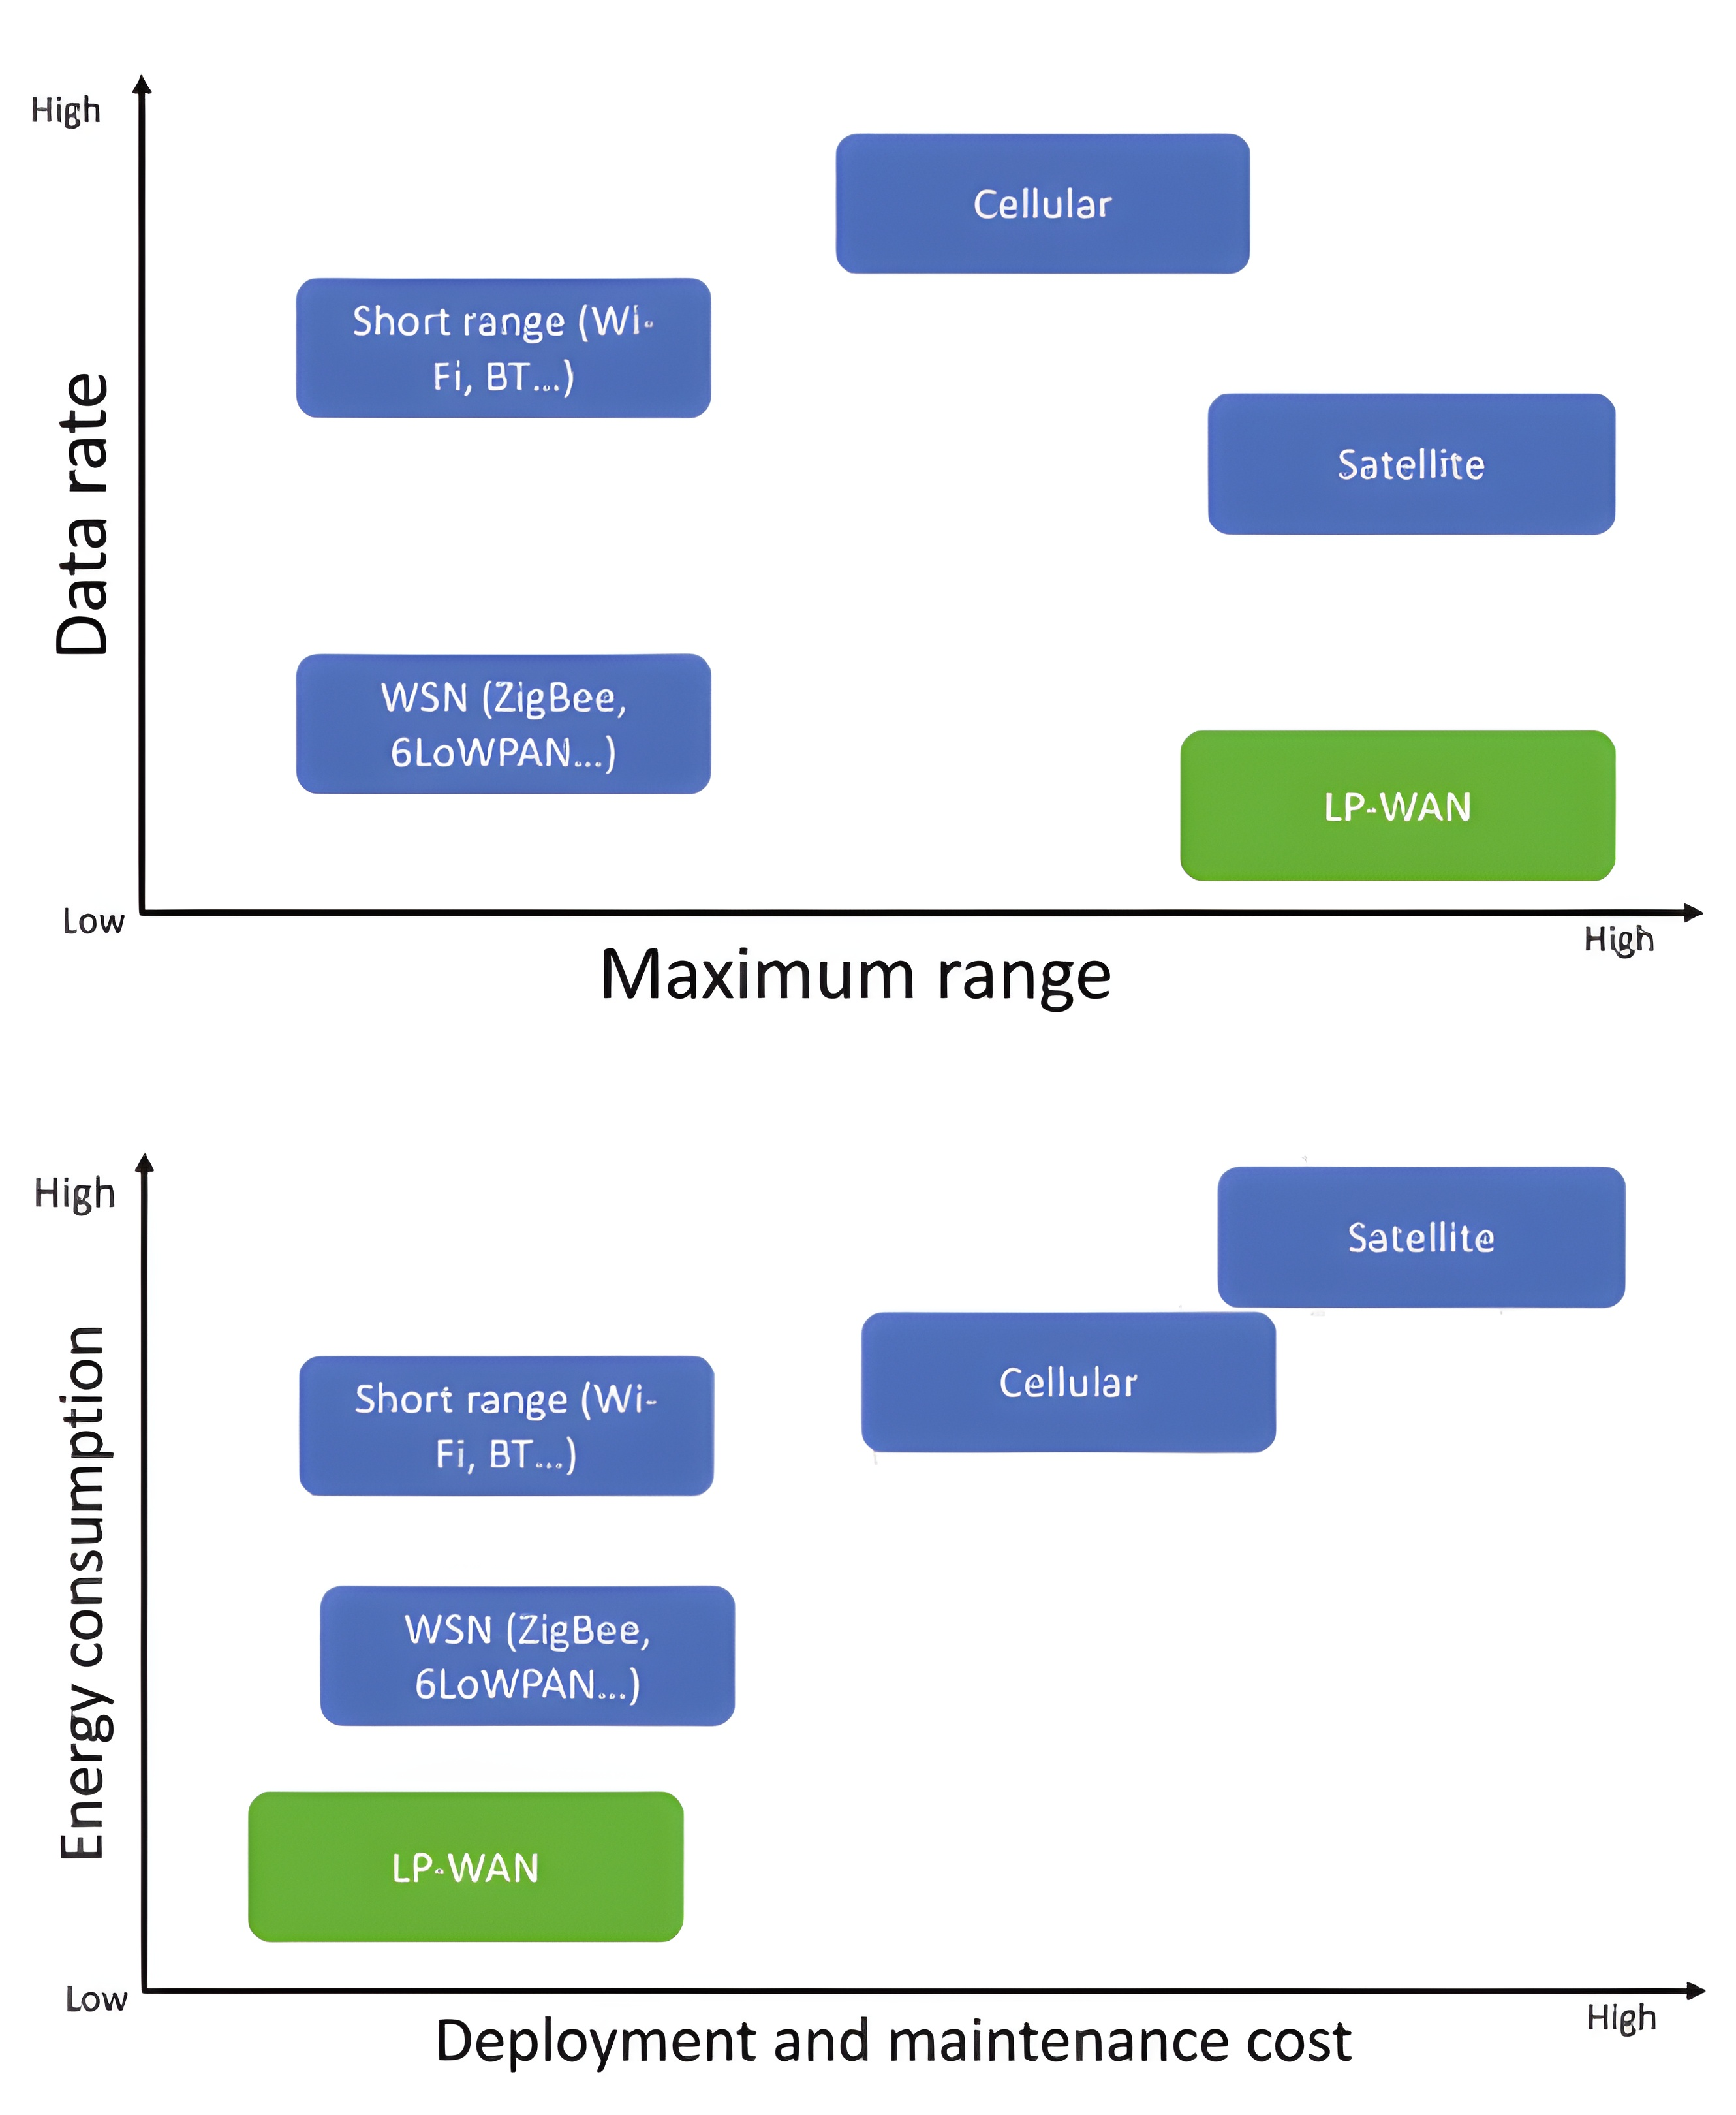
\includegraphics[scale=0.1]{Sections/Introduction/LP-WAN-Range.jpg}
\end{figure}
\end{comment}




\section{Aims and Objectives}

The aim of this project is to develop and deploy a prototype IoT architecture with the purpose of collecting data relevant to the health of the Griffith footbridge. This involves implementing the first five layers of the architecture which consist of the coding layer, perception layer, network layer, middle-ware layer and application layer. This deployment will be achieved through the testing and implementation of two prototypes.

The first prototype is designed for testing the software and the first three layers of the IoT architecture. Two Arduino MKRWAN 1300 devices will be used, one acting as the LoRa node (layer one and two) and the other acting as a pseudo LoRaWAN gateway (layer three). The first MKRWAN 1300 is equipped with an ADXL335 3-axis accelerometer and is placed on a metal beam. The beam is vibrated along the z-axis and the device samples the acceleration. The device finds the maximum frequency peak and maximum acceleration and transmits the data via a LoRa packet. The second device receives the LoRa packet and logs the data via a serial connection. The high level system diagram in figure \ref{Proto1HLSD} presents the desired implementation of this prototype. 

\begin{figure}[h]
	\centering
	\caption{Prototype 1 High Level System Diagram}
	\label{Proto1HLSD}
	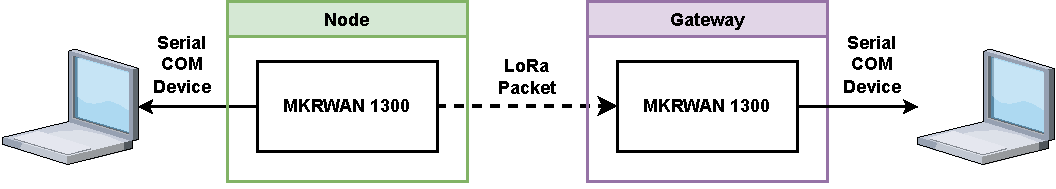
\includegraphics[scale=1]{Sections/Introduction/Prototype-1-High-Level.drawio.pdf}
\end{figure}

		The second prototype is designed for testing the software, PCB, enclosure and first five layers of the IoT architecture. The two MKRWAN 1300 devices are now both nodes and are implemented onto a custom designed PCB. This PCB is enclosed in a custom 3D printed enclosure and sits behind the guard rail of the Griffith foot bridge. The two nodes sample the maximum frequency and maximum acceleration of the bridge and transmit this data via LoRa packets to a Wisgate Edge Lite 2 LoRaWAN gateway. This gateway uploads the data via WIFI or Ethernet to the TNN cloud which acts as the middle-ware layer. --- APPLICATION LAYER WHAT IS THE IMPLEMENTATION --- Figure \ref{Proto2HLSD}
displays the high level system diagram for the second prototype. 

\begin{figure}[h] 
	\centering
	\caption{Prototype 2 High Level System Diagram}
	\label{Proto2HLSD}
	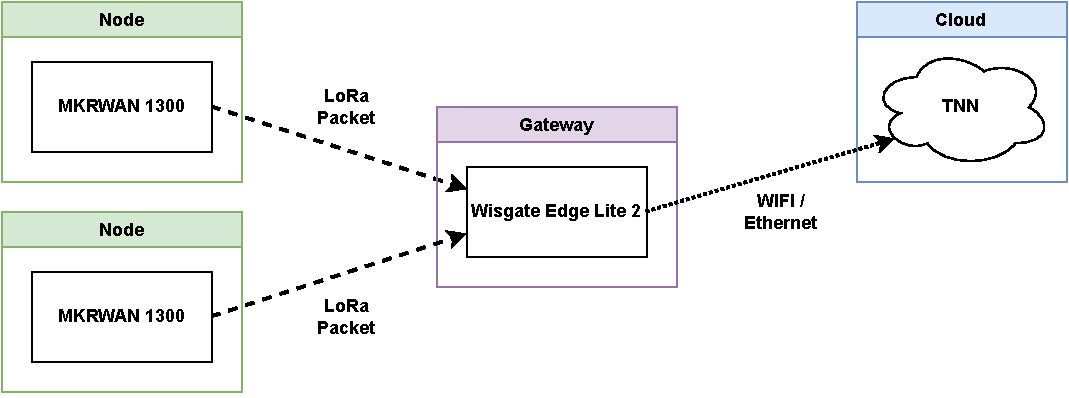
\includegraphics[scale=0.8]{Sections/Introduction/Prototype-2-High-Level.drawio.pdf}
\end{figure}

--- WHAT IS THE SUCCESS CRITERIA. SUCCESSFUL WHEN ??? ---

\newpage
\chapter{Review of Published Literature}
\section{Review of the Published Literature}
This literature review explores a variety of studies revolving around LoRaWAN and focuses on the fundamental end device setup, signal strength measurement, IoT cloud architecture and inherent limitations of the technology. LoRaWAN has gained traction for its promise of long-range, low-power solutions to WSNs which is critical for IoT applications. However, there are significant research gaps in the literature regarding the reliability and concistency of LoRaWAN in various environmental conditions and its practicality for applications requiring real time response. This review aims to evaluate these research gaps and evidence the design and optimization considerations for the LoRaWAN-based Structural Health Monitoring (SHM) deployment for the Griffith footbridge. The literature synthesized in this review is instrumental in shaping the approach and methodology of this research project. 

One application of LoRaWAN is in the field of Agro-Informatics, as demonstrated by Gehani et al. (2021) \cite{LoRa-Agro-Informatics}. Their research focused on utilizing LoRaWAN IoT architecture for the detection and classification of plant pathogens. The signal strength of the transmitted LoRa packets was evaluated through Received Signal Strength Indicator (RSSI) and Signal-to-Noise Ratio (SNR) at various depths from 0 cm to 60 cm. Their findings suggest that LoRa transmitters can function effectively provided the depth does not exceed 50 cm. A diagram of the experimental setup is shown in figure \ref{lora-bucket}. This research serves as a valuable foundation for designing the enclosure thickness that will be used in this project. 

\begin{figure}[h]
	\centering
	\caption{Experimental Setup for LoRa Node in Soil \cite{LoRa-Agro-Informatics}}
	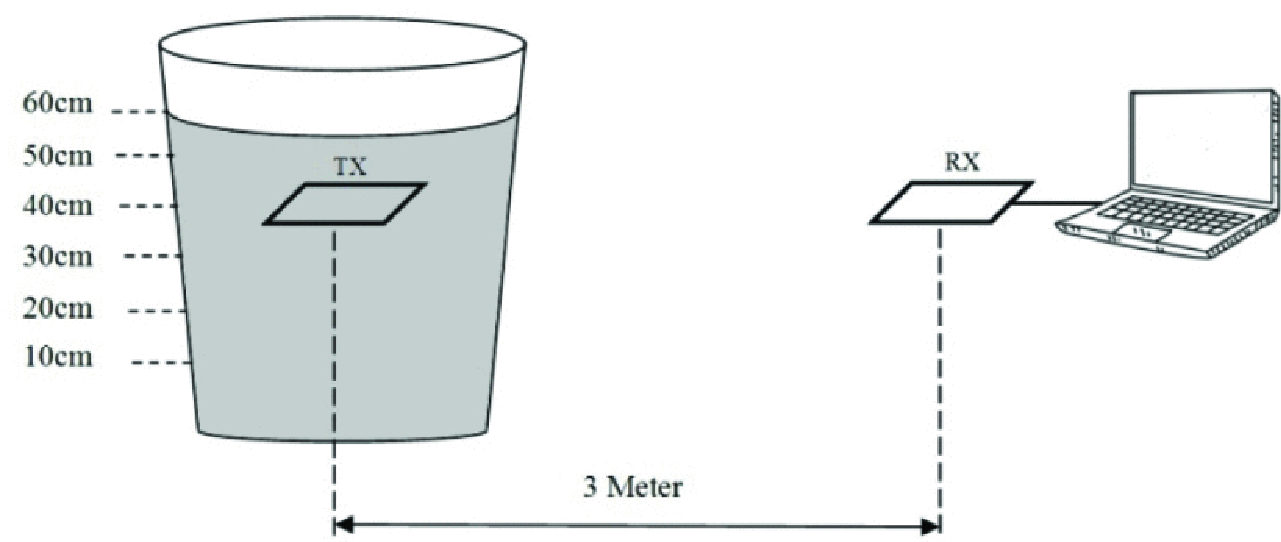
\includegraphics[scale=0.5]{Sections/Literature-Review/Lora-bucket.pdf}
	\label{lora-bucket}
\end{figure}

Fox et al. (2019) \cite{IoT-Regional-Service} expanded on the architecture of LoRaWAN-based IoT systems with a focus on wind turbine monitoring in Ireland. Their study comprised three main components: an end device, a gateway, and an IBM IoT cloud platform. This research demonstrated a comprehensive IoT cloud architecture deployment, covering real-time monitoring, concurrent read/write processes, and database service implementation. Despite the successful deployment, challenges such as LoRa's limited transmission capacity and application specific end device battery life were highlighted, emphasizing the need for future optimization. In terms of practical application, end devices must be optimized to strike a balance between computational load and current draw to achieve sufficient longevity. Figure \ref{Example-GUI} displays an example of a GUI displaying real time data visualization from the Red Node Cloud Foundry application flow within the IBM cloud. The LoRa payload is extracted, processed and displayed in an interface by assigning relative values to their respective interface nodes. With the knowledge gained from this research, the variables from the LoRa payload in this project will be extracted using Arduino IoT cloud variables, and an Arduino IoT cloud dashboard will be used to plot relevant time series data. The Arduino LoRaWAN Adaptive Data Rate (ADR) mechanism will be used in this project to optimise the airtime, data rate and power consumption of the LoRaWAN deployment. This will assist in striking the balance between computational load and current draw of the LoRa node. 

\begin{figure}[h]
	\centering
	\caption{Example of real time data visualization GUI \cite{IoT-Regional-Service}}
	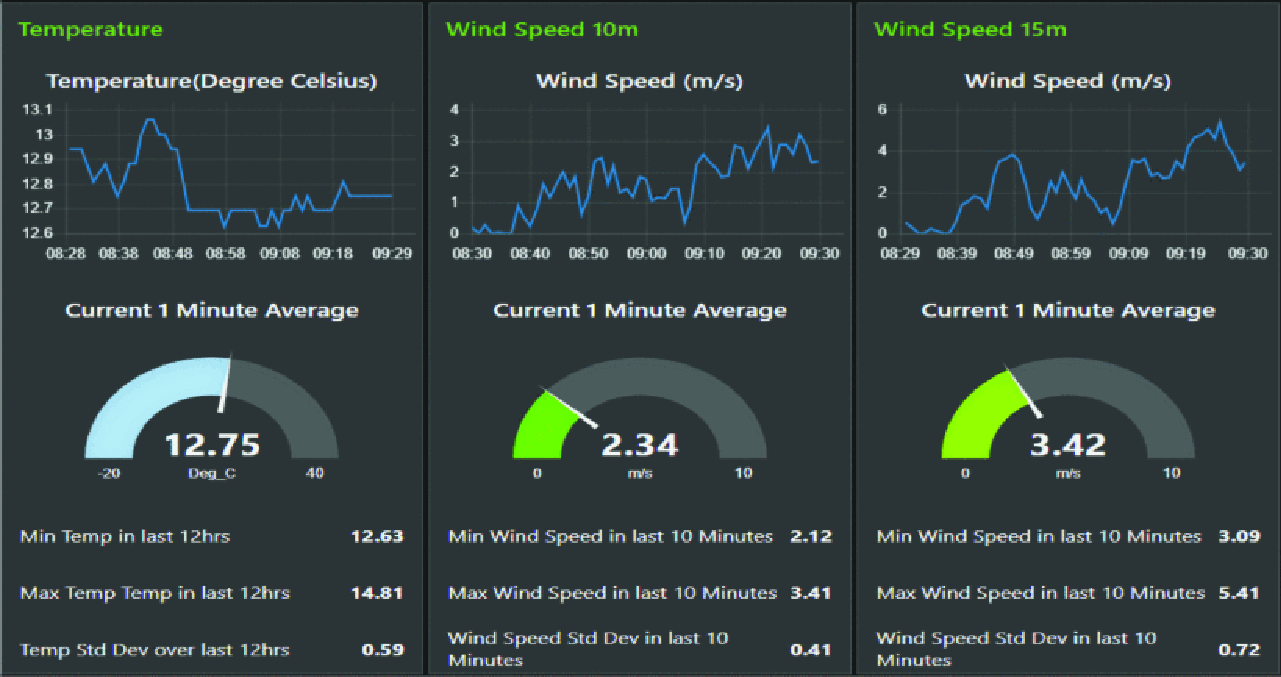
\includegraphics[scale=0.6]{Sections/Literature-Review/Example-GUI.pdf}
	\label{Example-GUI}
\end{figure}

In another exploration of LoRaWAN capabilities, Wildan et al. (2020) \cite{LoRa-Smart-Home} designed and implemented a GUI for smart home systems leveraging LoRa's long-range and low-power benefits. Information such as room temperature is transmitted to a LoRa server through a LoRa client, and is uploaded to a web server. The data is then stored in a database and displayed on a webpage which is accessible from various devices such as a smartphone and laptop. An interface application was created to allow user interaction with the webpage and control over various electronic devices such as lights, TV and air conditioning within the house. The system's performance was tested with a focus on the user experience, web application and delay. This testing was able to address a key limitation in LoRaWAN, the delay in data transmission, noting that while the system performance was generally robust, delays averaged 3.86 seconds. This makes LoRaWAN generally limited for systems that require close to real-time responses. In relation to the smart home, operating the lights and TV with a 3.86 second delay is both significant and noticeable. In its current state this system is functional, but will inevitably invoke hesitancy for mainstream adoption due to an installation cost for a user experience that is not seamless. The delay time evidenced in this study has resulted in avoiding unnecessary downlink messages for this project. This project will only focus on receiving uplink messages with only necessary downlink acknowledgements to avoid the restriction of a delayed response time. 

Maziero et al. (2019) \cite{Monitoring-Electric-Parameters} deployed a real-time monitoring system for tracking electrical quantities at the Federal University of Santa Maria campus. Utilizing Grafana software, they created a panel for tracking both electrical and connectivity metrics, demonstrating the effectiveness of combining LoRaWAN technology and application layer monitoring software for real-time data acquisition and visualization. The study highlights the potential scalability of this system in the sense of feeding data stored in the monitoring center to algorithms capable of autonomously handling the distribution network of electrical metrics, for example automatically altering voltage based on state estimations. It was evident in the research that the ability to monitor electrical quantities in the application layer allowed for the capability of better management and informed decision making based on a holistic interpretation of the distribution network. Figure \ref{Electrical-Monitoring-System} displays the design for the electrical monitoring system and the process of receiving data from The Things Network (TNN) applications and transmitting payloads to a web-based user interface via MQTT and HTTP messaging protocols. The system design of this study gives an excellent context for the chosen implementation of TNN for this project. In this project TNN applications will instead communicate with the Arduino IoT cloud using cloud variables which will be used to plot data on the web-based Arduino cloud dashboard. 

\begin{figure}[h]
	\centering
	\caption{IoT architecture for monitoring electrical quantities \cite{Monitoring-Electric-Parameters}}
	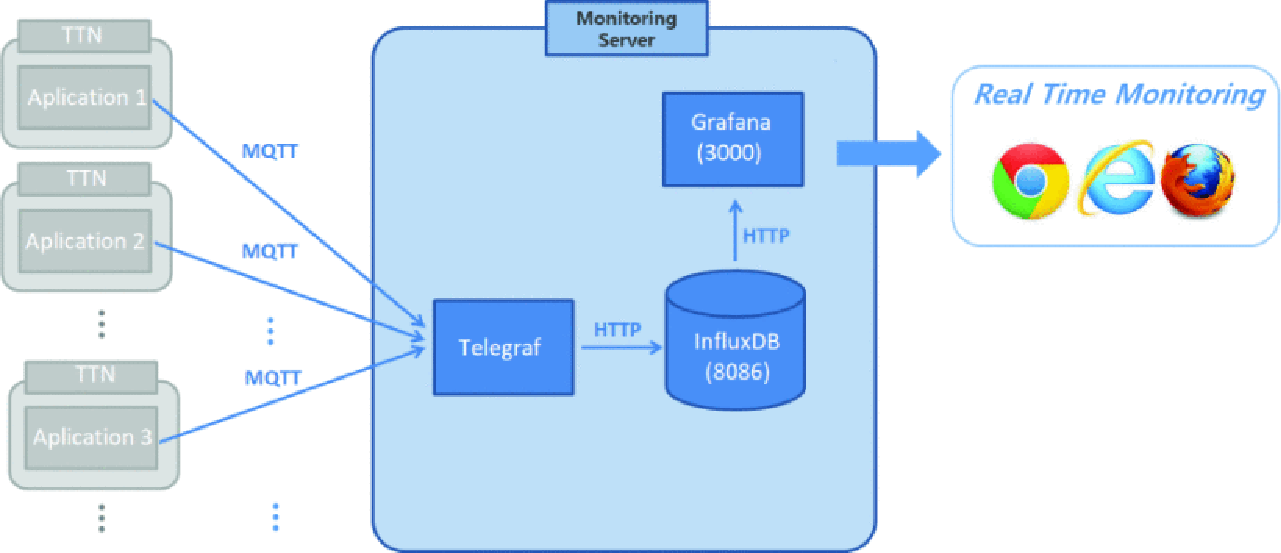
\includegraphics[scale=0.5]{Sections/Literature-Review/Electrical-Monitoring-System.pdf}
	\label{Electrical-Monitoring-System}
\end{figure}

In a study examining the performance of a Smart Gateway network architecture, the authors conducted a series of test focusing on throughput and packet loss \cite{Monitoring-System-Smart-Gateway}. The throughput was found to be inconsistent across a different number of clients where the system was found to have a lower average throughput compared to other LoRaWAN systems due to additional required processing steps. The extra processing steps were attributed to Quality of Service (QoS) parameters, such as measuring packet loss and throughput, processing client data and web server services running on the gateway. The study found a significant packet loss especially when operating with two clients. On average, the system exhibited packet loss of 26\% across a 1-meter range which is a significantly high drop compared to other LoRaWAN implementations. Despite the range limitations, the study concluded that the gateway could support up to 5 clients registering and requesting data automatically, and run LoRa communication alongside the user interface of the information system simultaneously. In light of these findings, this report intends to use the ADR mechanism to automatically optimize QoS since it dynamically chooses the best spreading factor (SF) to send LoRa packets over. Additionally, the gateway used in this project will act as a base station and use the Arduino IoT Cloud and The Things Network (TNN) to handle the network and application layer, removing unnecessary gateway computations. 

Wixted et al. (2016) \cite{LoRa-WSN} conducted reliability testing and discovered a successful connection and acknowledgement request between an end device and gateway across all spreading factors was found to be only 42\% at a distance of 1.9km. After introducing a second gateway this connection rate rose to 70\% and with the introduction of Internet Control Message protocol (ICMP) pings the full connection rate rose to 95.5\%. It was also found that connection was completely lost in isolated stairwells indicating that LoRaWAN is sensitive to obstructions. Thanks to the findings of this research, the deployment of the LoRaWAN system in this project will focus on a short-range setup with minimal obstruction, and focus on the holistic deployment of the IoT architecture. 

In a paper presenting an online test bed for LoRa development, the correlation between packet RSSI and distance was measured \cite{Dandelion-Testbed}. 5 LoRa nodes were placed at distances 500m, 1000m and 1200m away from the gateway, where the nodes placed 100m and 1200m were blocked by urban and natural obstacles. It was found that a low spreading factor (SF) results in a reduction of the packet reception rate (PRR). SF7 was the lowest spreading factor used and was confirmed to only support packet transmission at very low distance. The study concluded that RSSI decreases with distance and that this relationship is directly influenced by the environment, obstacles and spreading factor used for transmission. Various models can be used to model the relationship between RSSI and distance, but as evidenced in figure \ref{rssi-distance-model} the Bor model was closest in predicting correlation. To investigate the RSSI and SNR in this project, the values will be extracted from TNN and plotted over time series. This will further assist in gaining an understanding of the fluctuation of signal strength at a fixed distance from the Griffith footbridge. 

\begin{figure}[h]
	\centering
	\caption{Modelling RSSI-distance correlation. Green represents real data. \cite{Dandelion-Testbed}}
	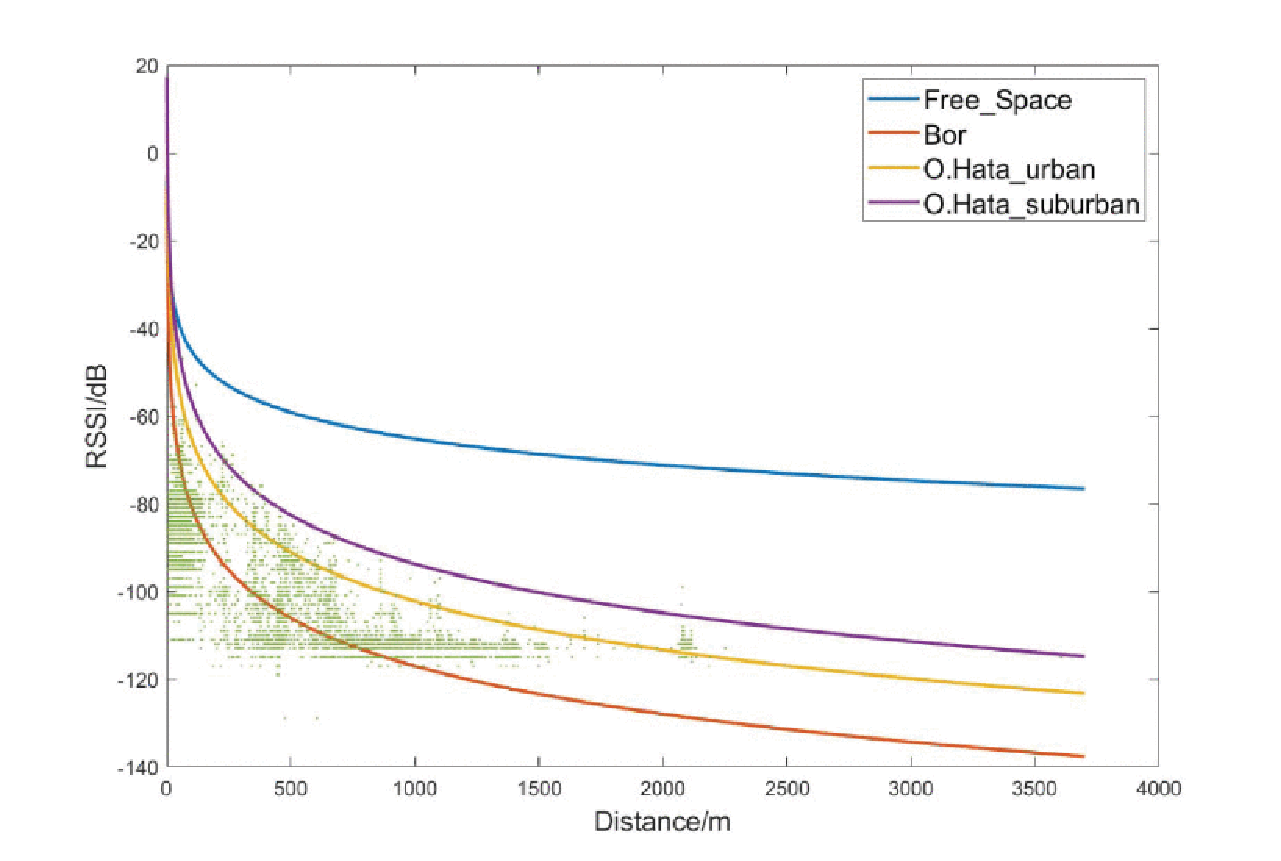
\includegraphics[scale=0.5]{Sections/Literature-Review/rssi-distance-model.pdf}
	\label{rssi-distance-model}
\end{figure}

Jang et al. in 2010 \cite{SHM-Korea} reports the deployment of 70 wireless smart sensor networks (WSSNs) and two base stations on the Jindo Bridge in South Korea. Each sensor facilitates 3-axis acceleration measurement and offers a test bed for structural health monitoring (SHM). Cho et al. in 2010 \cite{WSSN-Korean-Bridge} analysed data collected from these WSSNs, comparing these results to existing acceleration data from a wired monitoring system. The acceleration data collected from the deck and pylons of the bridge revealed a significant acceleration due to vehicle traffic. Vertical and cable vibrations were found to be significant enough for mode extraction and the estimated tension forces for 10 cables were found to lie within a 4\% difference of the previous site inspections using wired monitoring systems. The frequencies of the higher modes were found to exceed those predicted in the finite element (FE) model by less than 16\%, indicating the benefit of WSSN data collection for verifying and amending simulated models. The PSD of the 2007 site inspection using the wired monitoring system is shown in figure \ref{PSD-Wired}. This gives an excellent insight for the expected PSD frequency peaks of the Griffith footbridge, indicating that a maximum peak of approximately 2Hz may appear. 

\begin{figure}[!htb]
	\centering
	\caption{PSD of vertical acceleration with wired monitoring system \cite{WSSN-Korean-Bridge}}
	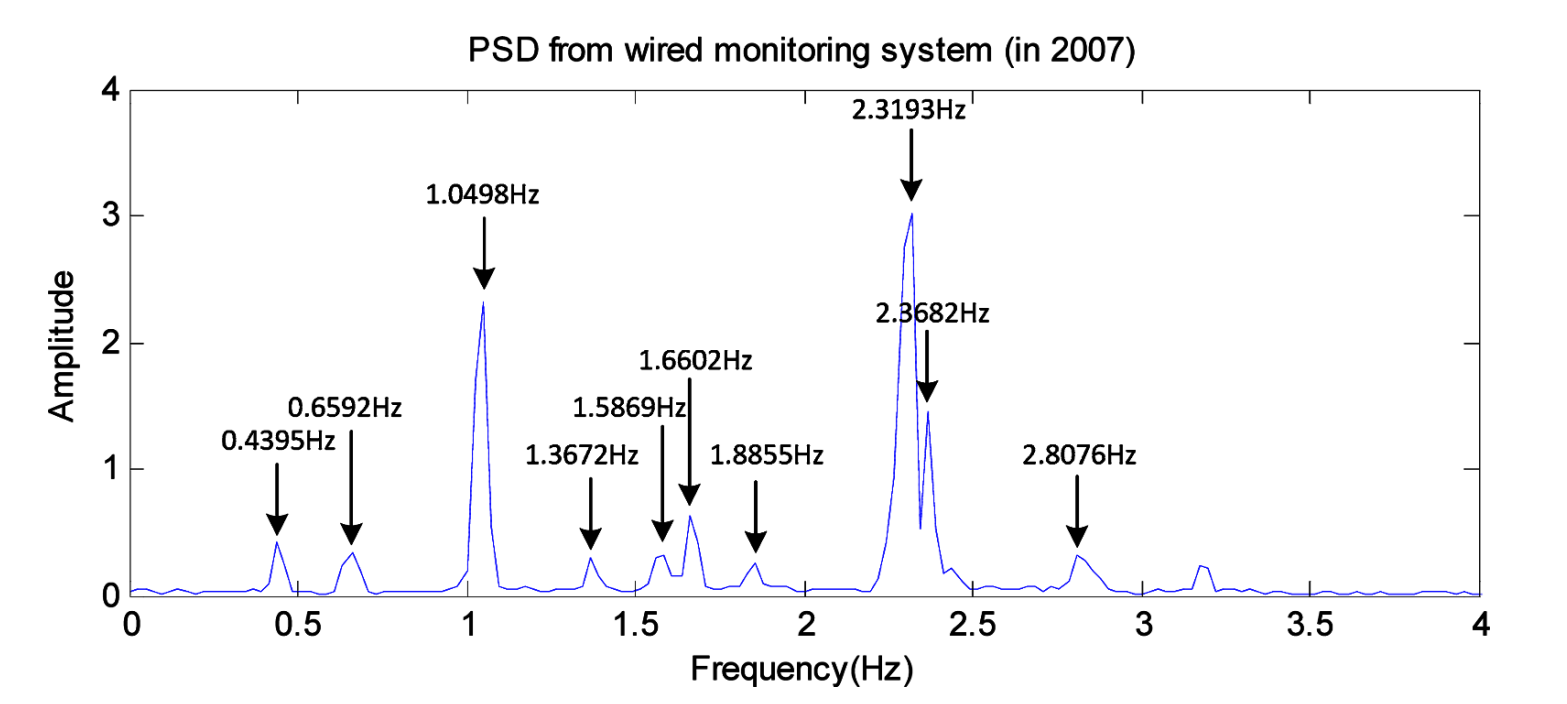
\includegraphics[scale=0.35]{Sections/Literature-Review/bridge-wired-psd.png}
	\label{PSD-Wired}
\end{figure}

The existing literature on LoRaWAN exemplifies the versatility and potential of this technology in various IoT applications, including those demanding long range and low power consumption. Several limitations including the inconsistencies in packet loss, throughput and connectivity, coupled with significant data transmission delay, as outlined in table \ref{Lit-Summary-Table}, present substantial challenges, especially for real-time data analysis and applications requiring consistent downlink messages. Such findings underscore the need for an in-depth understanding of LoRaWAN's performance to address these limitations in this project's system design. 




\begin{table}[!hbt]
\begin{tabular}{|c|l|l|}
\hline
\rowcolor[HTML]{C0C0C0} 
\textbf{Reference}                                               & \multicolumn{1}{c|}{\cellcolor[HTML]{C0C0C0}\textbf{Significant Contribution}}                                                     & \multicolumn{1}{c|}{\cellcolor[HTML]{C0C0C0}\textbf{Limitation}}                                                                                         \\ \hline
\begin{tabular}[c]{@{}c@{}}Gehani et al.\\ (2021)\end{tabular}   & \begin{tabular}[c]{@{}l@{}}LoRa Transmitters can function \\ effectively up to a depth of 50 cm\\ in soil.\end{tabular}            & \begin{tabular}[c]{@{}l@{}}Only 3 m distance between \\ transmitting and receiving \\ node.\end{tabular}                                                 \\ \hline
\begin{tabular}[c]{@{}c@{}}Fox et al.\\ (2019)\end{tabular}      & \begin{tabular}[c]{@{}l@{}}Comprehensive IoT cloud \\ architecture deployment.\end{tabular}                                        & \begin{tabular}[c]{@{}l@{}}Limited transmission\\ capacity and end device \\ battery life.\end{tabular}                                                  \\ \hline
\begin{tabular}[c]{@{}c@{}}Wildan et al. \\ (2020)\end{tabular}  & \begin{tabular}[c]{@{}l@{}}Designed and implemented a GUI \\ for smart home systems leveraging \\ LoRa.\end{tabular}               & \begin{tabular}[c]{@{}l@{}}Data transmission delay \\ averaged 3.86 seconds.\end{tabular}                                                                \\ \hline
\begin{tabular}[c]{@{}c@{}}Maziero et al.\\ (2019)\end{tabular}  & \begin{tabular}[c]{@{}l@{}}Real-time monitoring system for \\ tracking electrical quantities.\end{tabular}                         & \begin{tabular}[c]{@{}l@{}}No explanation for smart \\ meters with packet delivery \\ less than 95\%.\end{tabular}                                       \\ \hline
\begin{tabular}[c]{@{}c@{}}Eridani et al. \\ (2019)\end{tabular} & \begin{tabular}[c]{@{}l@{}}Conducted a series of tests focusing \\ on throughput and packet loss.\end{tabular}                     & \begin{tabular}[c]{@{}l@{}}Inconsistent throughput \\ and significant packet loss.\end{tabular}                                                          \\ \hline
\begin{tabular}[c]{@{}c@{}}Wixted et al. \\ (2016)\end{tabular}  & \begin{tabular}[c]{@{}l@{}}Successful connection and \\ acknowledgement request between \\ an end device and gateway.\end{tabular} & \begin{tabular}[c]{@{}l@{}}Connection was completely \\ lost in isolated stairwells \\ and low with only one gateway.\end{tabular}                       \\ \hline
\begin{tabular}[c]{@{}c@{}}Wang et al. \\ (2019)\end{tabular}    & \begin{tabular}[c]{@{}l@{}}Correlation between packet RSSI \\ and distance was measured.\end{tabular}                              & \begin{tabular}[c]{@{}l@{}}RSSI decreases with distance \\ and is directly influenced by \\ environment, obstacles and \\ spreading factor.\end{tabular} \\ \hline
\begin{tabular}[c]{@{}c@{}}Jang et al. \\ (2010)\end{tabular}    & \begin{tabular}[c]{@{}l@{}}Large scale deployment of WSSNs \\ and two base stations on the Jindo\\ Bridge.\end{tabular}            & \begin{tabular}[c]{@{}l@{}}Linear relationship between \\ number of requested data \\ points and communication time.\end{tabular}                        \\ \hline
\begin{tabular}[c]{@{}c@{}}Cho et al. \\ (2020)\end{tabular}     & \begin{tabular}[c]{@{}l@{}}Analysed data collected from the\\ WSSNs.\end{tabular}                                                  & \begin{tabular}[c]{@{}l@{}}Independent WSSN analysis \\ required due to no \\ synchronization.\end{tabular}                                              \\ \hline
\end{tabular}
\caption{Summary of Reviewed Literature}
\label{Lit-Summary-Table}
\end{table}

In the context of SHM, LoRaWAN presents a compelling alternative to traditional WSNs, such as Wi-Fi, Bluetooth and Zigbee, offering superior range and adaptability whilst satisfying low power requirements and the potential for flexible sensor placement. However, the highlighted limitations from the literature must be carefully addressed in the design of this LoRaWAN-based SHM system. This project will seek to tackle the presented challenges by focusing on the design optimization for the Griffith footbridge monitoring system. In particular, the aim is to strike a balance between computational load, power consumption and data transmission delay whilst ensuring robust and reliable system performance. 
\chapter{Design Process}
\section{Prototype testing}
\chapter{Prototype Testing}
\section{Testing Methodology and Criteria}
\subsection{Prototype 1: Beam Test}

The purpose of the beam test was to test the functionality of the software on prototype one, and to validate the first mode fundamental frequency from the Strand7 FE simulation. This test involved fastening a large metal beam to a clamp, and securing the node device to the end of the beam using elastic bands. As outlined in the system diagram in figure \ref{proto1-sys-diagram}, the node and gateway devices were first physically connected to a laptop as serial COM devices. The test setup can be seen in figure \ref{beam-test-setup}. 

\begin{figure}[H] 
	\centering
	\caption{Laboratory Beam Test Setup}
	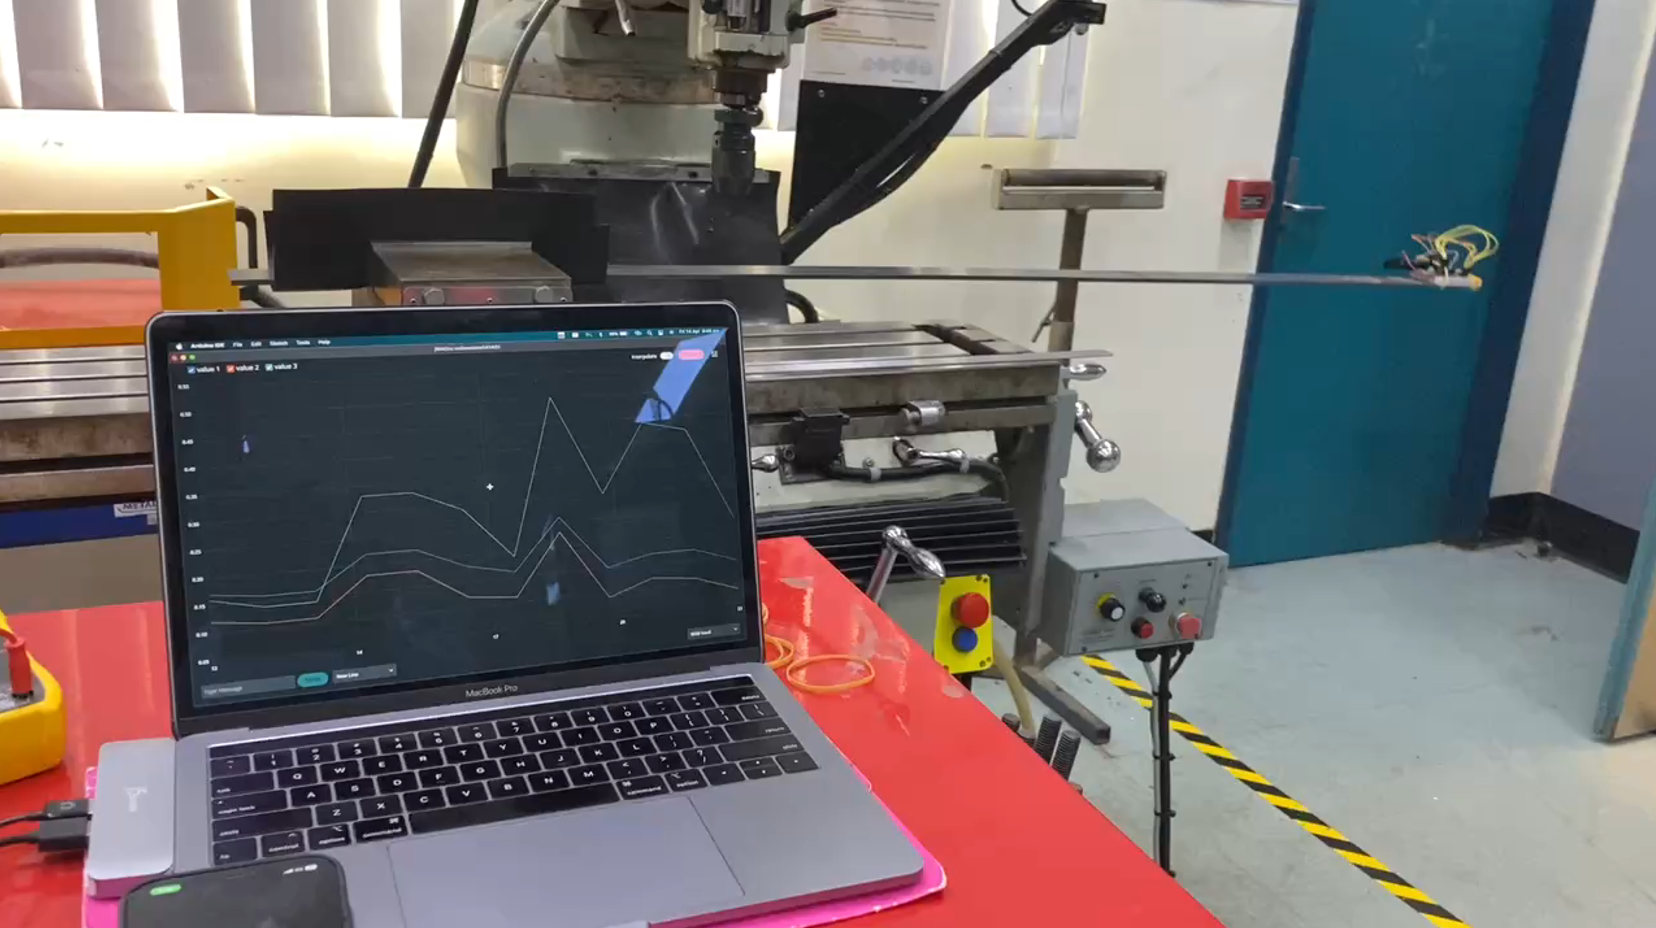
\includegraphics[width=\textwidth]{Sections/Prototype-Testing/beam-test-setup.png}
	\label{beam-test-setup}
\end{figure}

Initially, the noise threshold values in the acceleration processing function were tuned through trial and error. The live serial plot in Arduino IDE assisted in tuning these parameters to a final value of 0.7 for the x-axis, 0.9 for the y-axis and 0.1 for the z-axis. The beam was then pushed down 15cm and released. Once the noise thresholds were acceptable, the first test was conducted. 

\subsubsection{Prototype 1: Test 1}
Test one involved two participants, one to monitor the laptop and run the software and another to push the beam down. The first test was conducted with both devices connected to the laptop via USB. The node device was fastened to the beam and the reset button was pushed, calibrating the device. The node device on the beam can be seen in figure \ref{node-beam-test}. The sender and receiver Python logging scripts were executed on the laptop, as seen in figure \ref{laptop-beam-test}, and the beam was released. The test ran for approximately two minutes until the beam reached a stationary state. At this moment the logging programs were ended and the sender and receiver Python plotting scripts were executed. The names of each logging file was input by the user and the raw acceleration, maximum acceleration and peak frequency were displayed in a pyplot graph. These graphs were named and saved as PNG files. 

\begin{figure}[H]
	\centering
	\begin{subfigure}{.5\textwidth}
		\centering 
		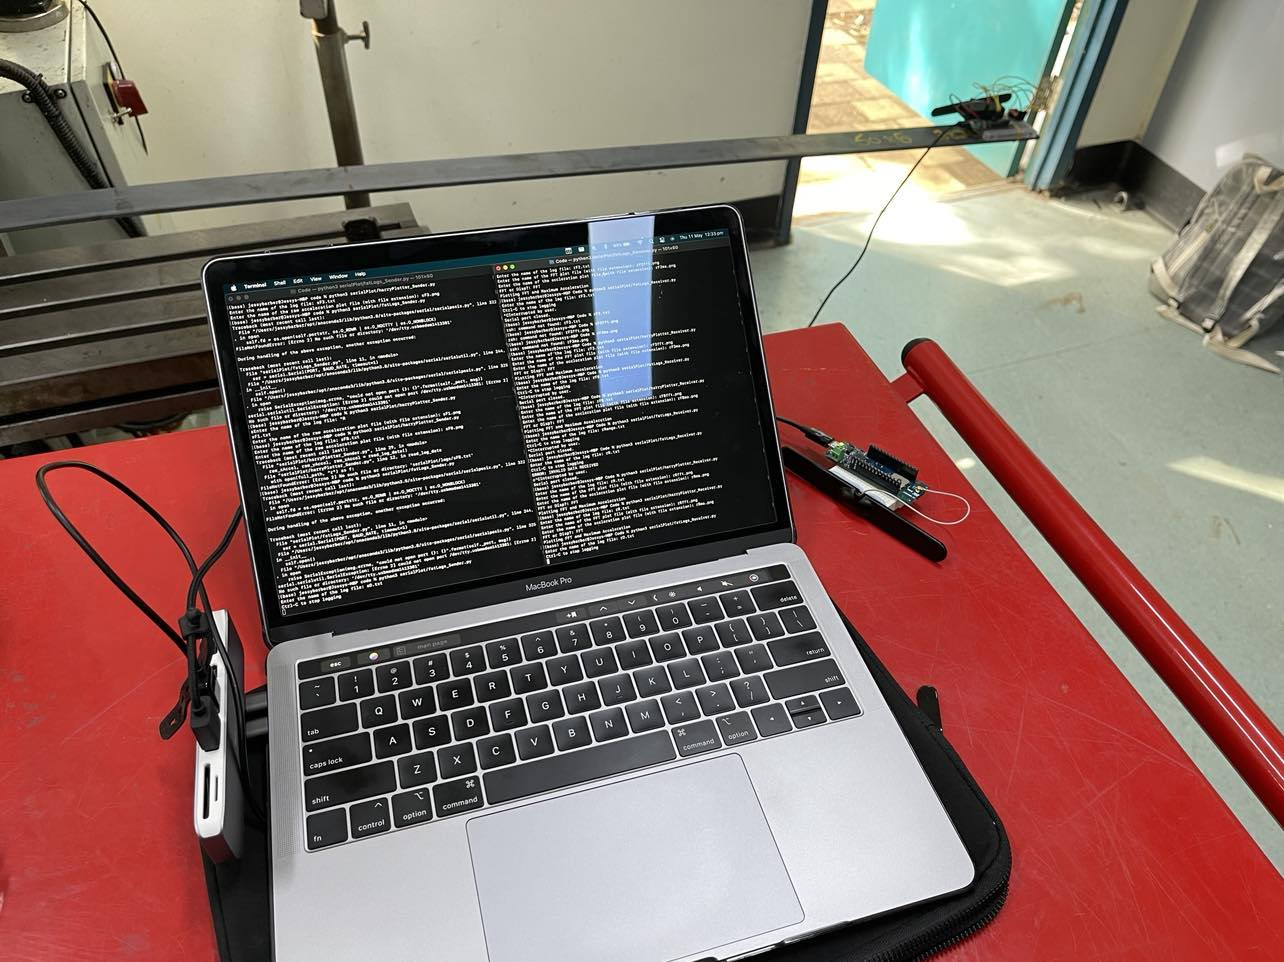
\includegraphics[scale=0.15]{Sections/Prototype-Testing/laptop-beam-test.jpg}
		\caption{Logging Python Scripts}
		\label{laptop-beam-test}
	\end{subfigure}%
	\begin{subfigure}{.25\textwidth}
		\centering
		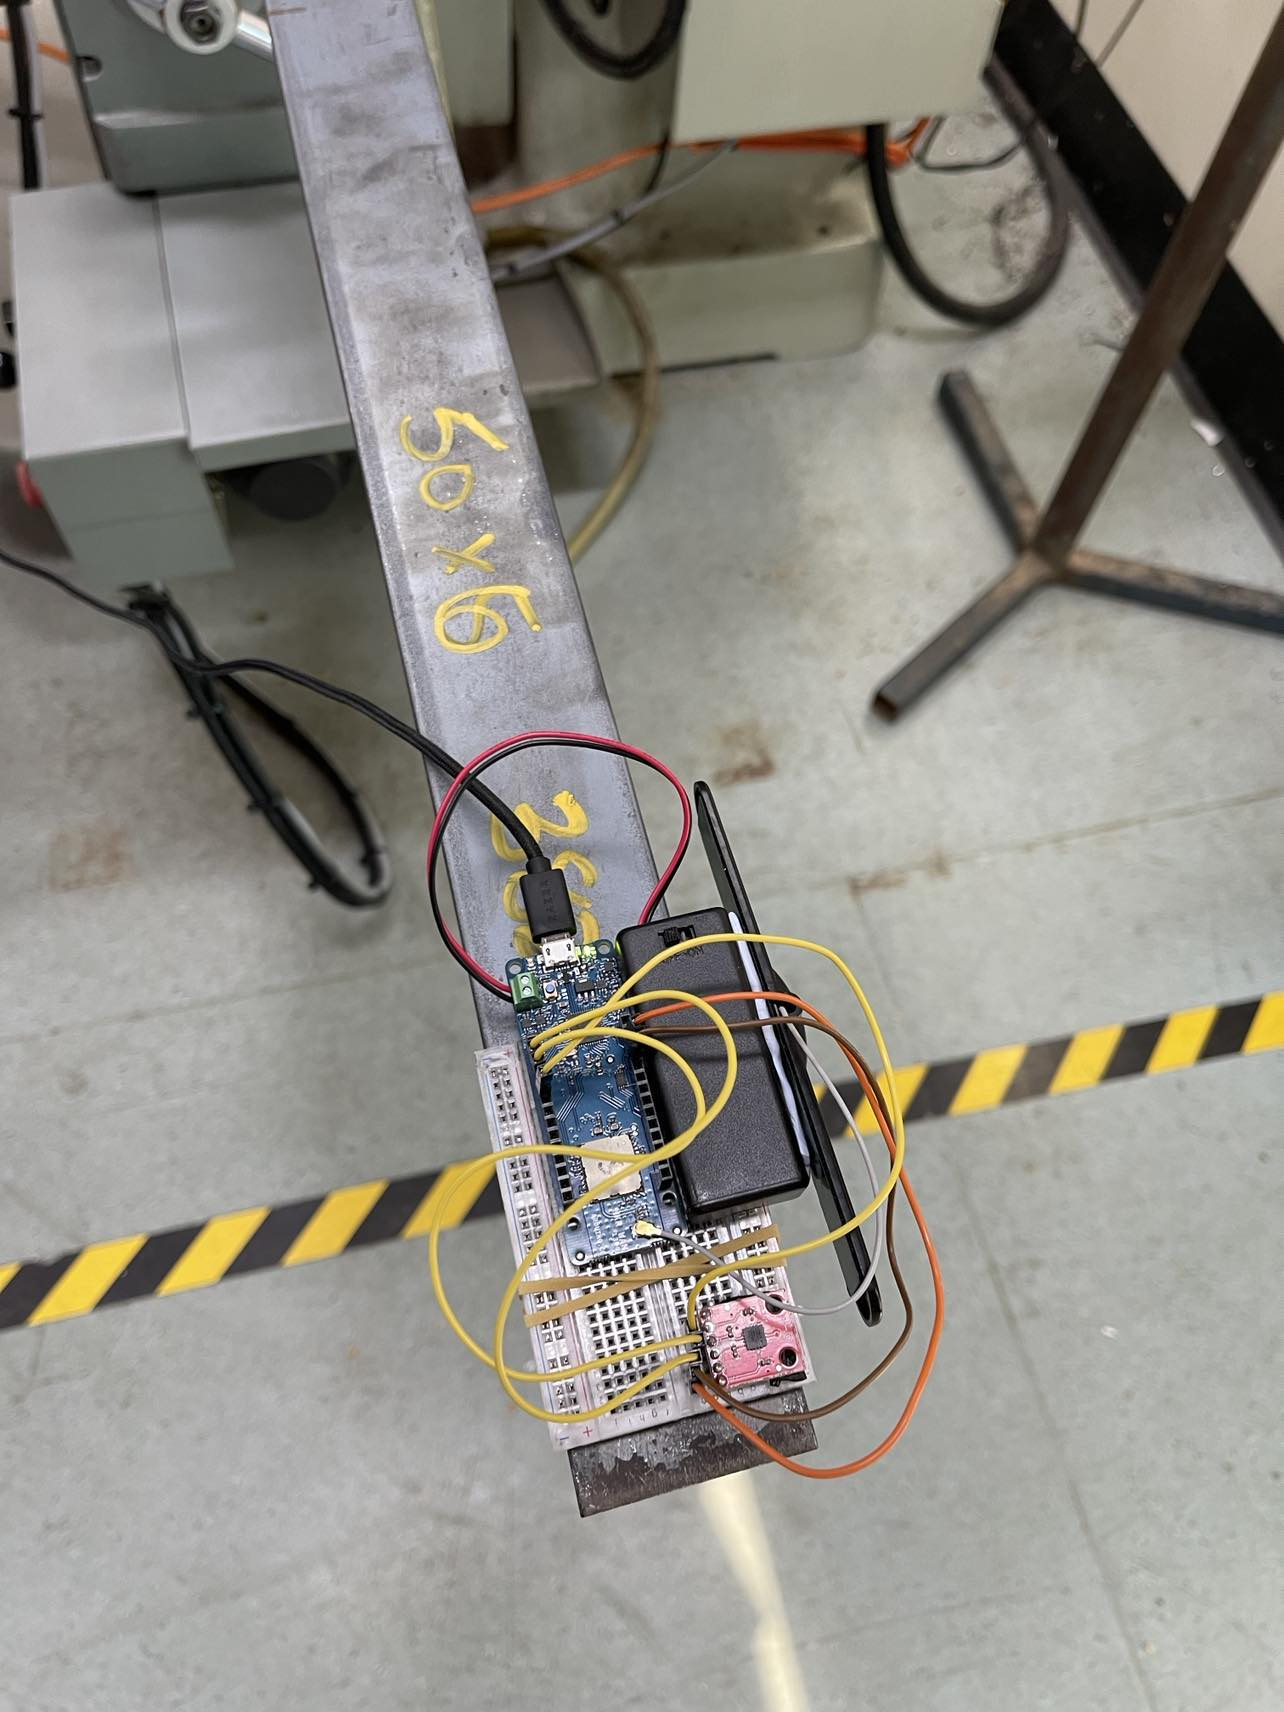
\includegraphics[scale=0.1]{Sections/Prototype-Testing/node-beam-test.jpg}
		\caption{Node Device on Beam}
		\label{node-beam-test}
	\end{subfigure}
	\caption{Close Up of Laptop and Node with Serial Connection in Beam Test}
	\label{close-beam-test}
\end{figure}

\subsubsection{Prototype 1: Test 1 Results}
Figure \ref{proto1-test1-ra} shows the raw acceleration from the serial connection between the node device and laptop and figures \ref{proto1-test1-ma} and \ref{proto1-test1-f} show the maximum acceleration and maximum frequency from the serial connection between the gateway device and the laptop. The raw and maximum acceleration are characteristic of the beam accelerating with maximum displacement and decaying over time to the stationary position. The peak frequency from the FFT is 2.4 Hz which matches the first mode fundamental frequency achieved in the Strand7 FE simulation shown in figures \ref{strand7-simulation} and \ref{strand7-results}. This verifies that the FFT computation can accurately identify the maximum peak frequency. 

\begin{figure}[H]
	\centering
	\caption{Beam Test FE Simulation}
	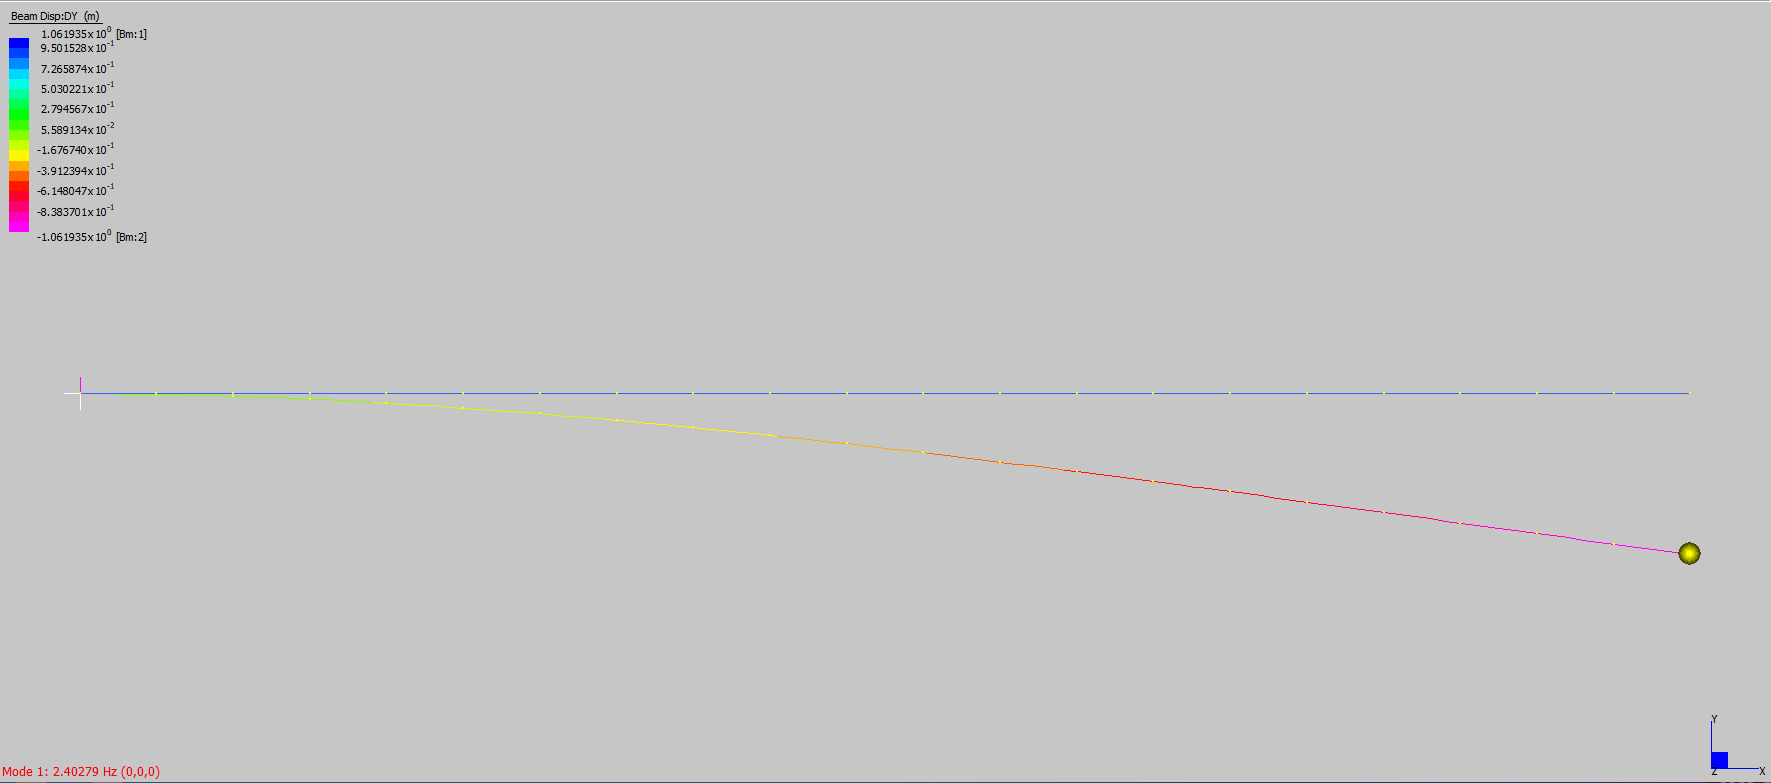
\includegraphics[width=\textwidth]{Sections/Prototype-Testing/strand7-simulation.png}
	\label{strand7-simulation}
\end{figure}

\begin{figure}[H]
	\centering
	\caption{Beam Test FE Simulation Results}
	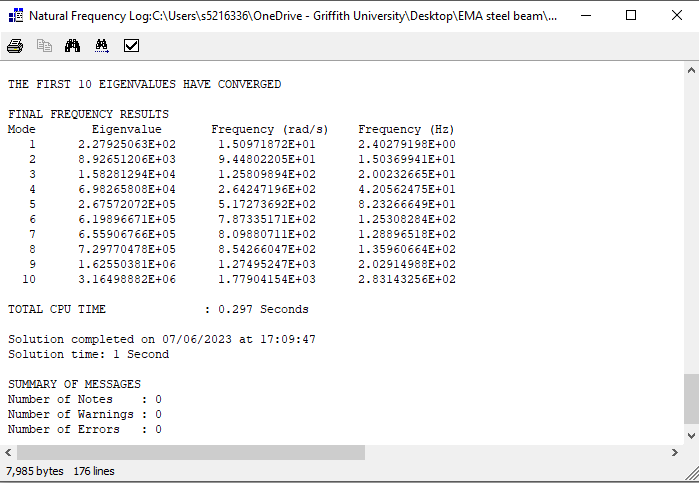
\includegraphics[width=\textwidth]{Sections/Prototype-Testing/strand7-results.png}
	\label{strand7-results}
\end{figure}

\begin{figure}[H]
	\centering
	\caption{Prototype 1: Test 1 Raw Acceleration}
	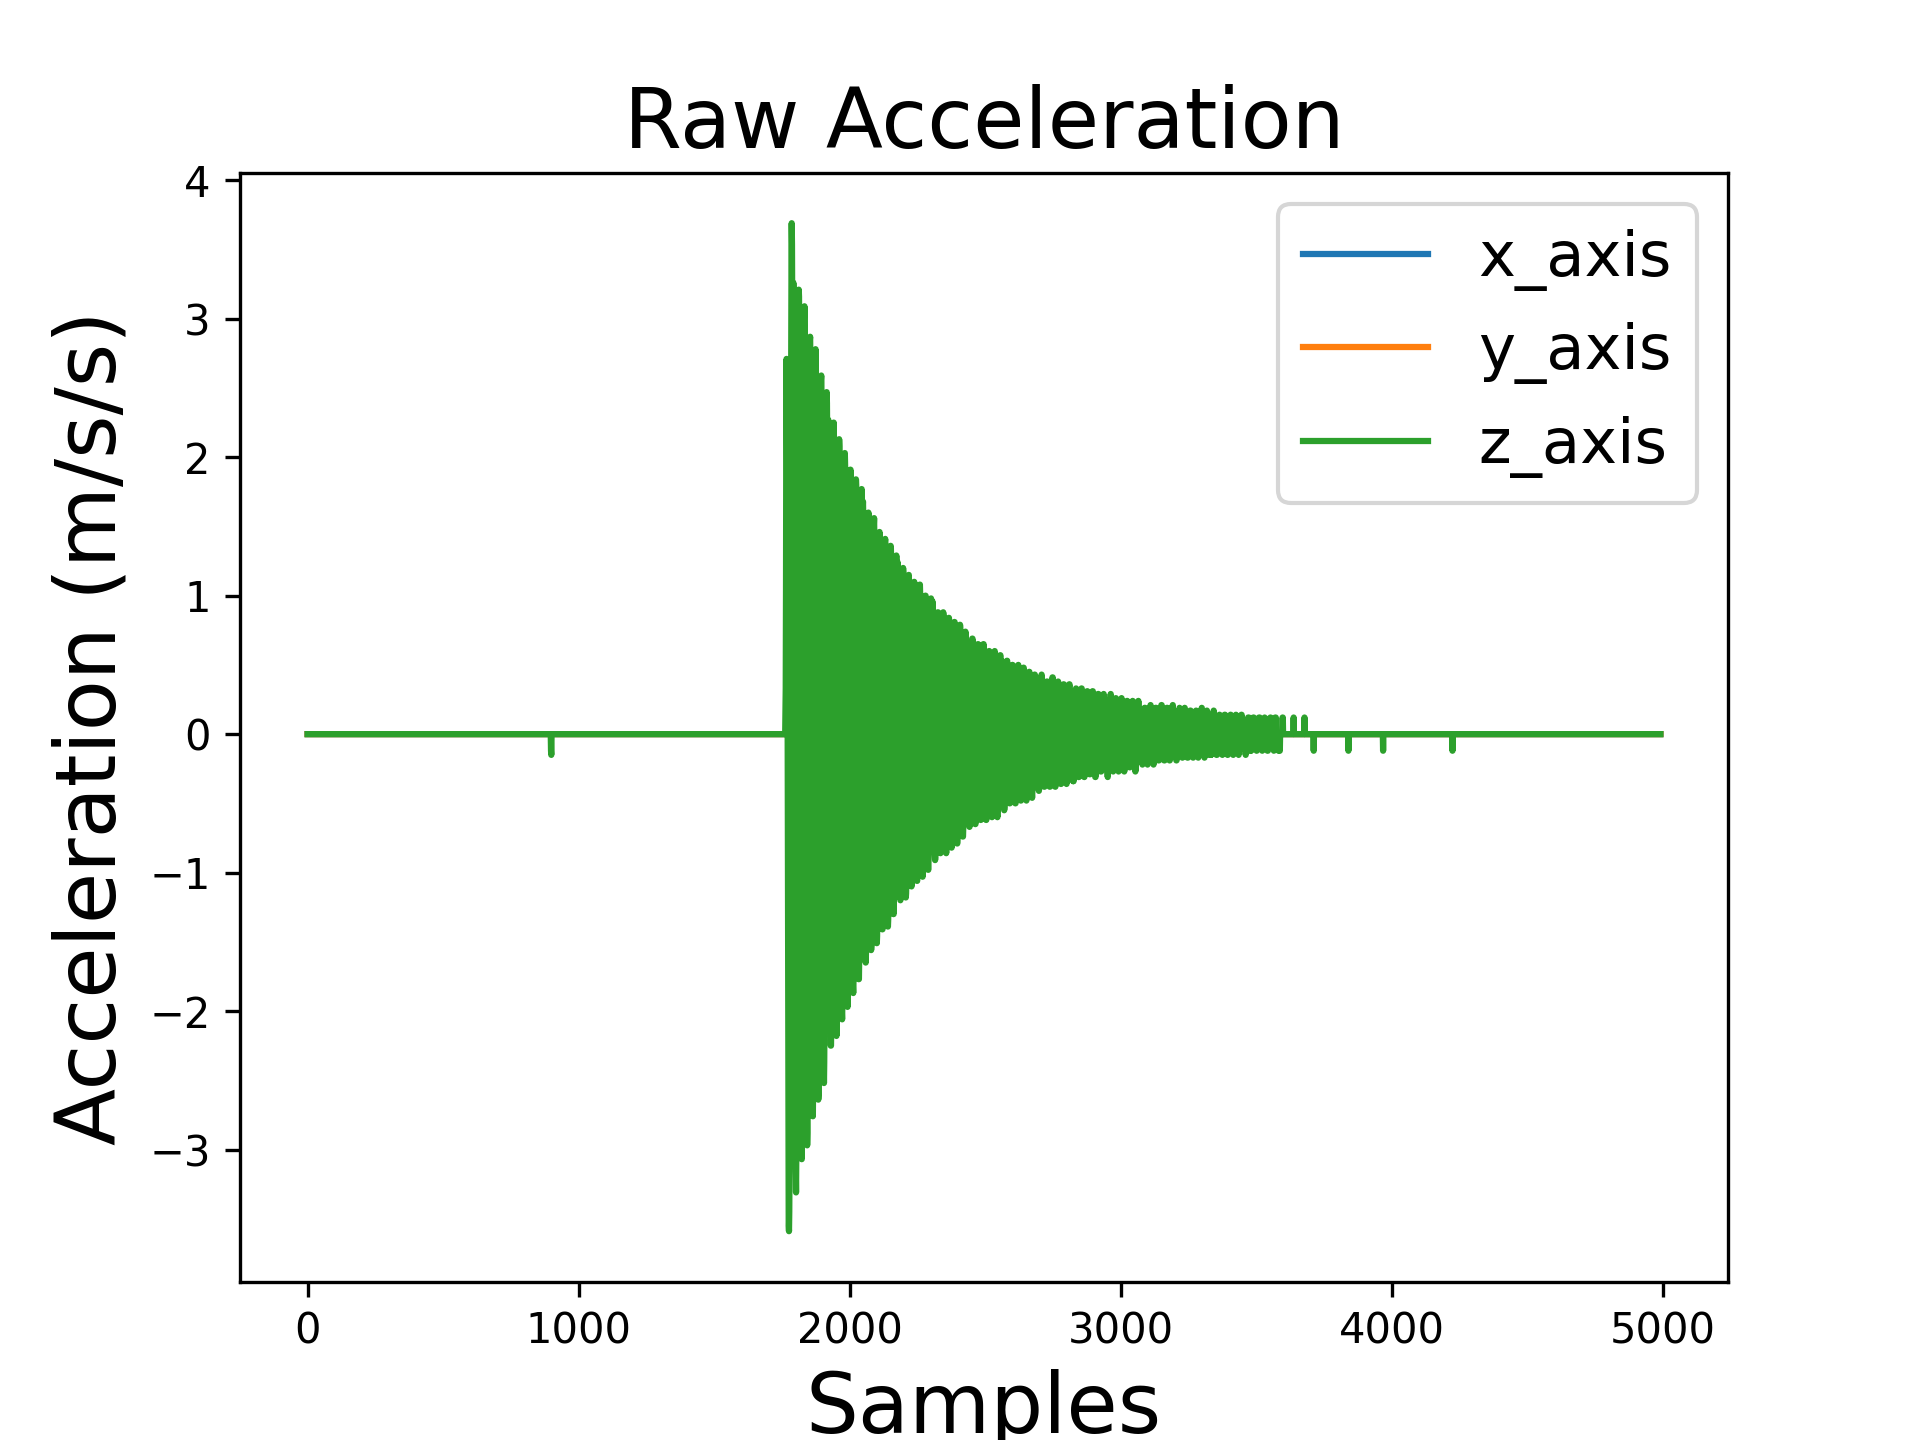
\includegraphics[width=.9\textwidth]{Sections/Prototype-Testing/PosterRA.png}
	\label{proto1-test1-ra}
\end{figure}

\begin{figure}[H]
	\centering
	\caption{Prototype 1: Test 1 Maximum Acceleration}
	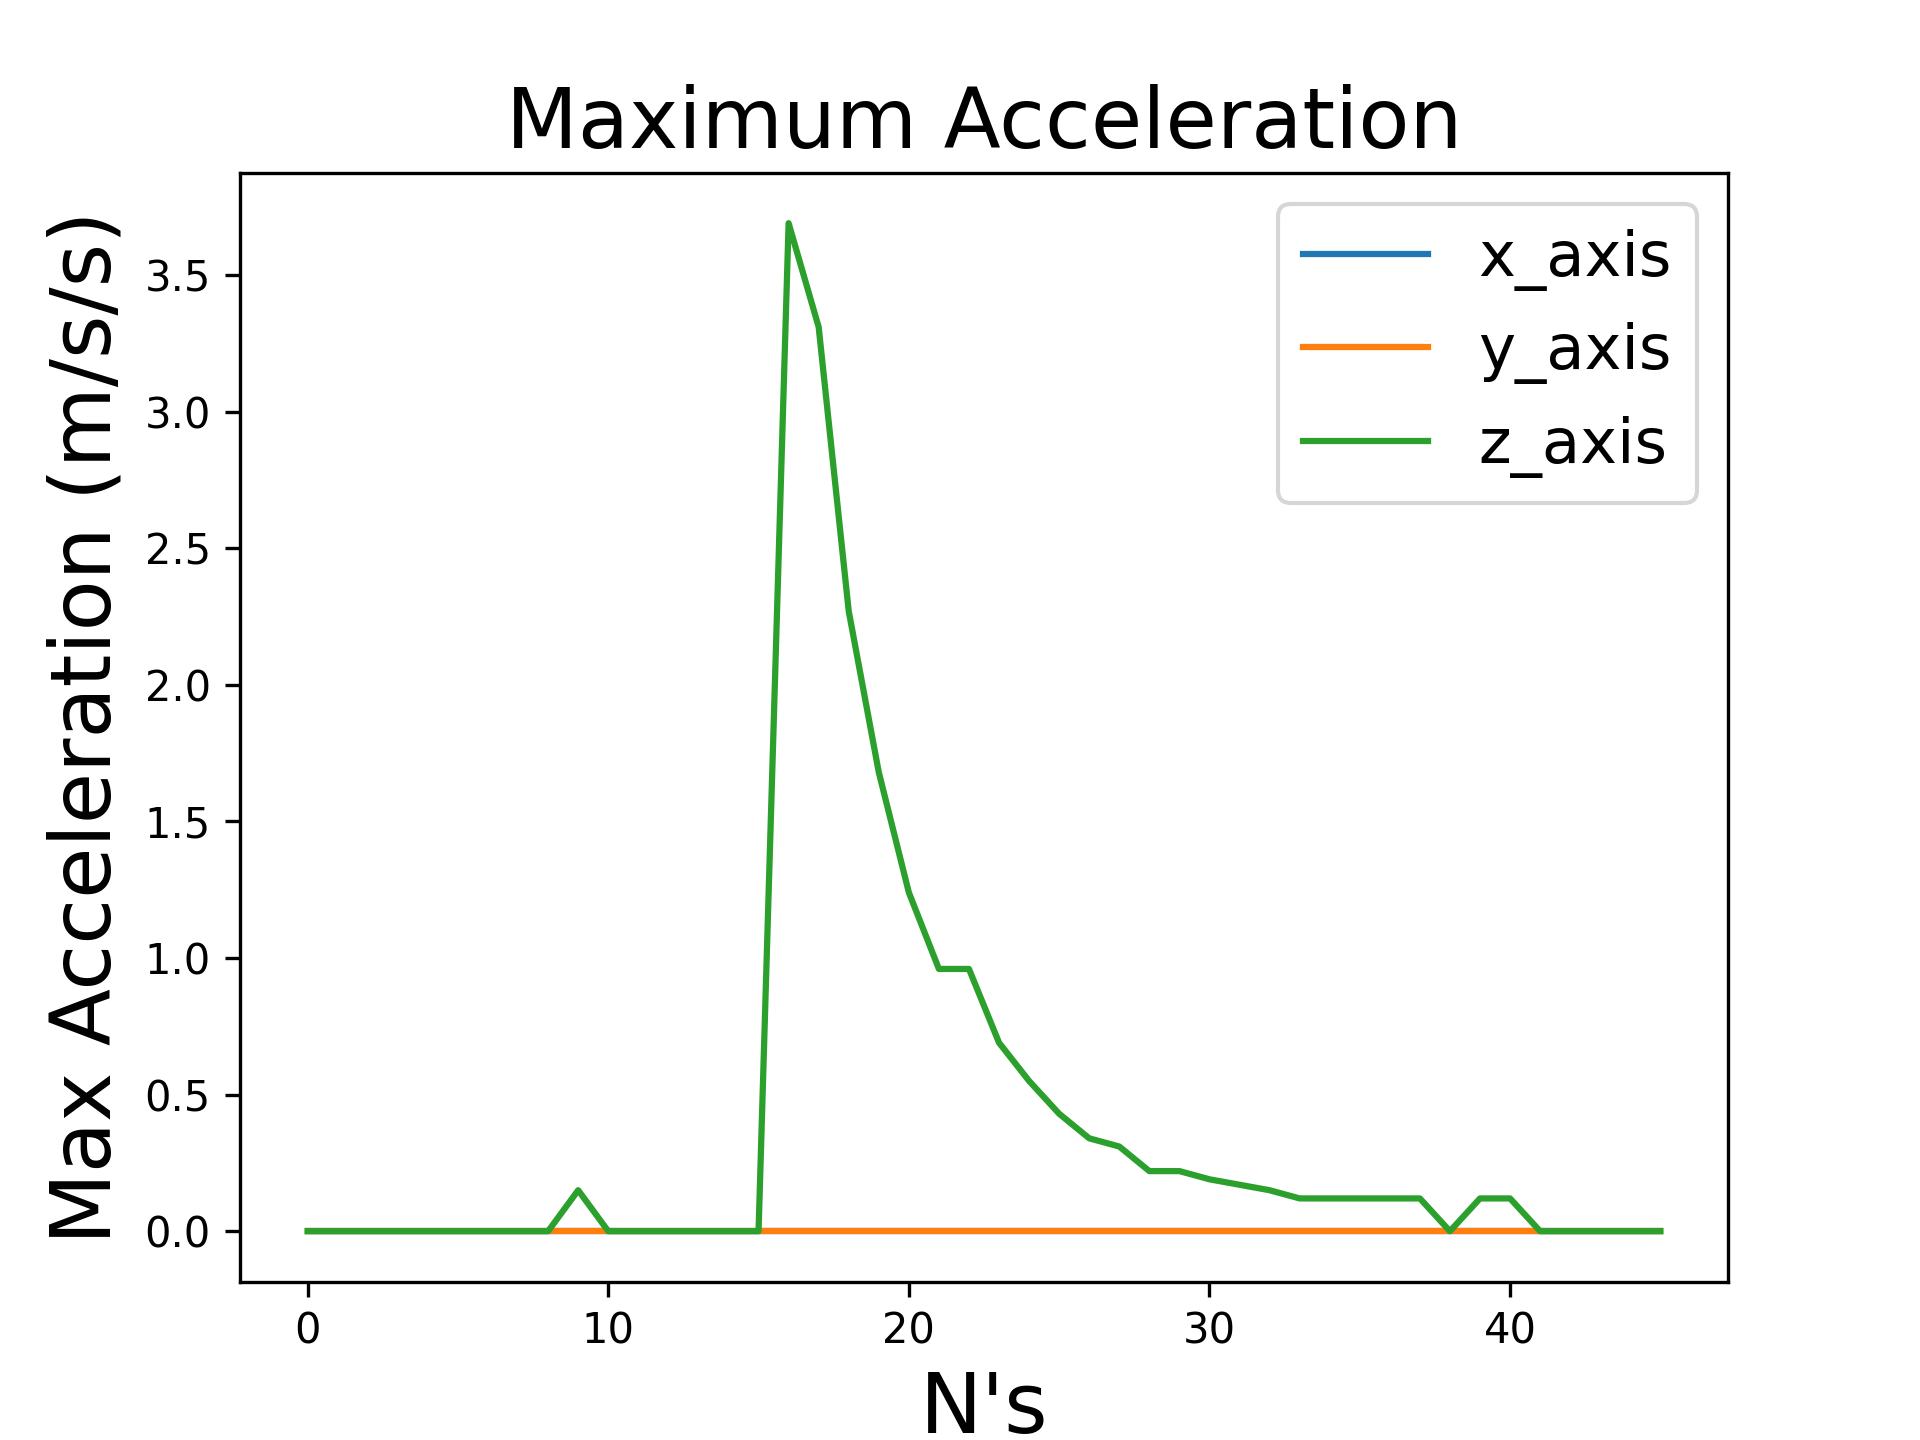
\includegraphics[width=.9\textwidth]{Sections/Prototype-Testing/PosterMA.png}
	\label{proto1-test1-ma}
\end{figure}

\begin{figure}[H]
	\centering
	\caption{Prototype 1: Test 1 Maximum Frequency}
	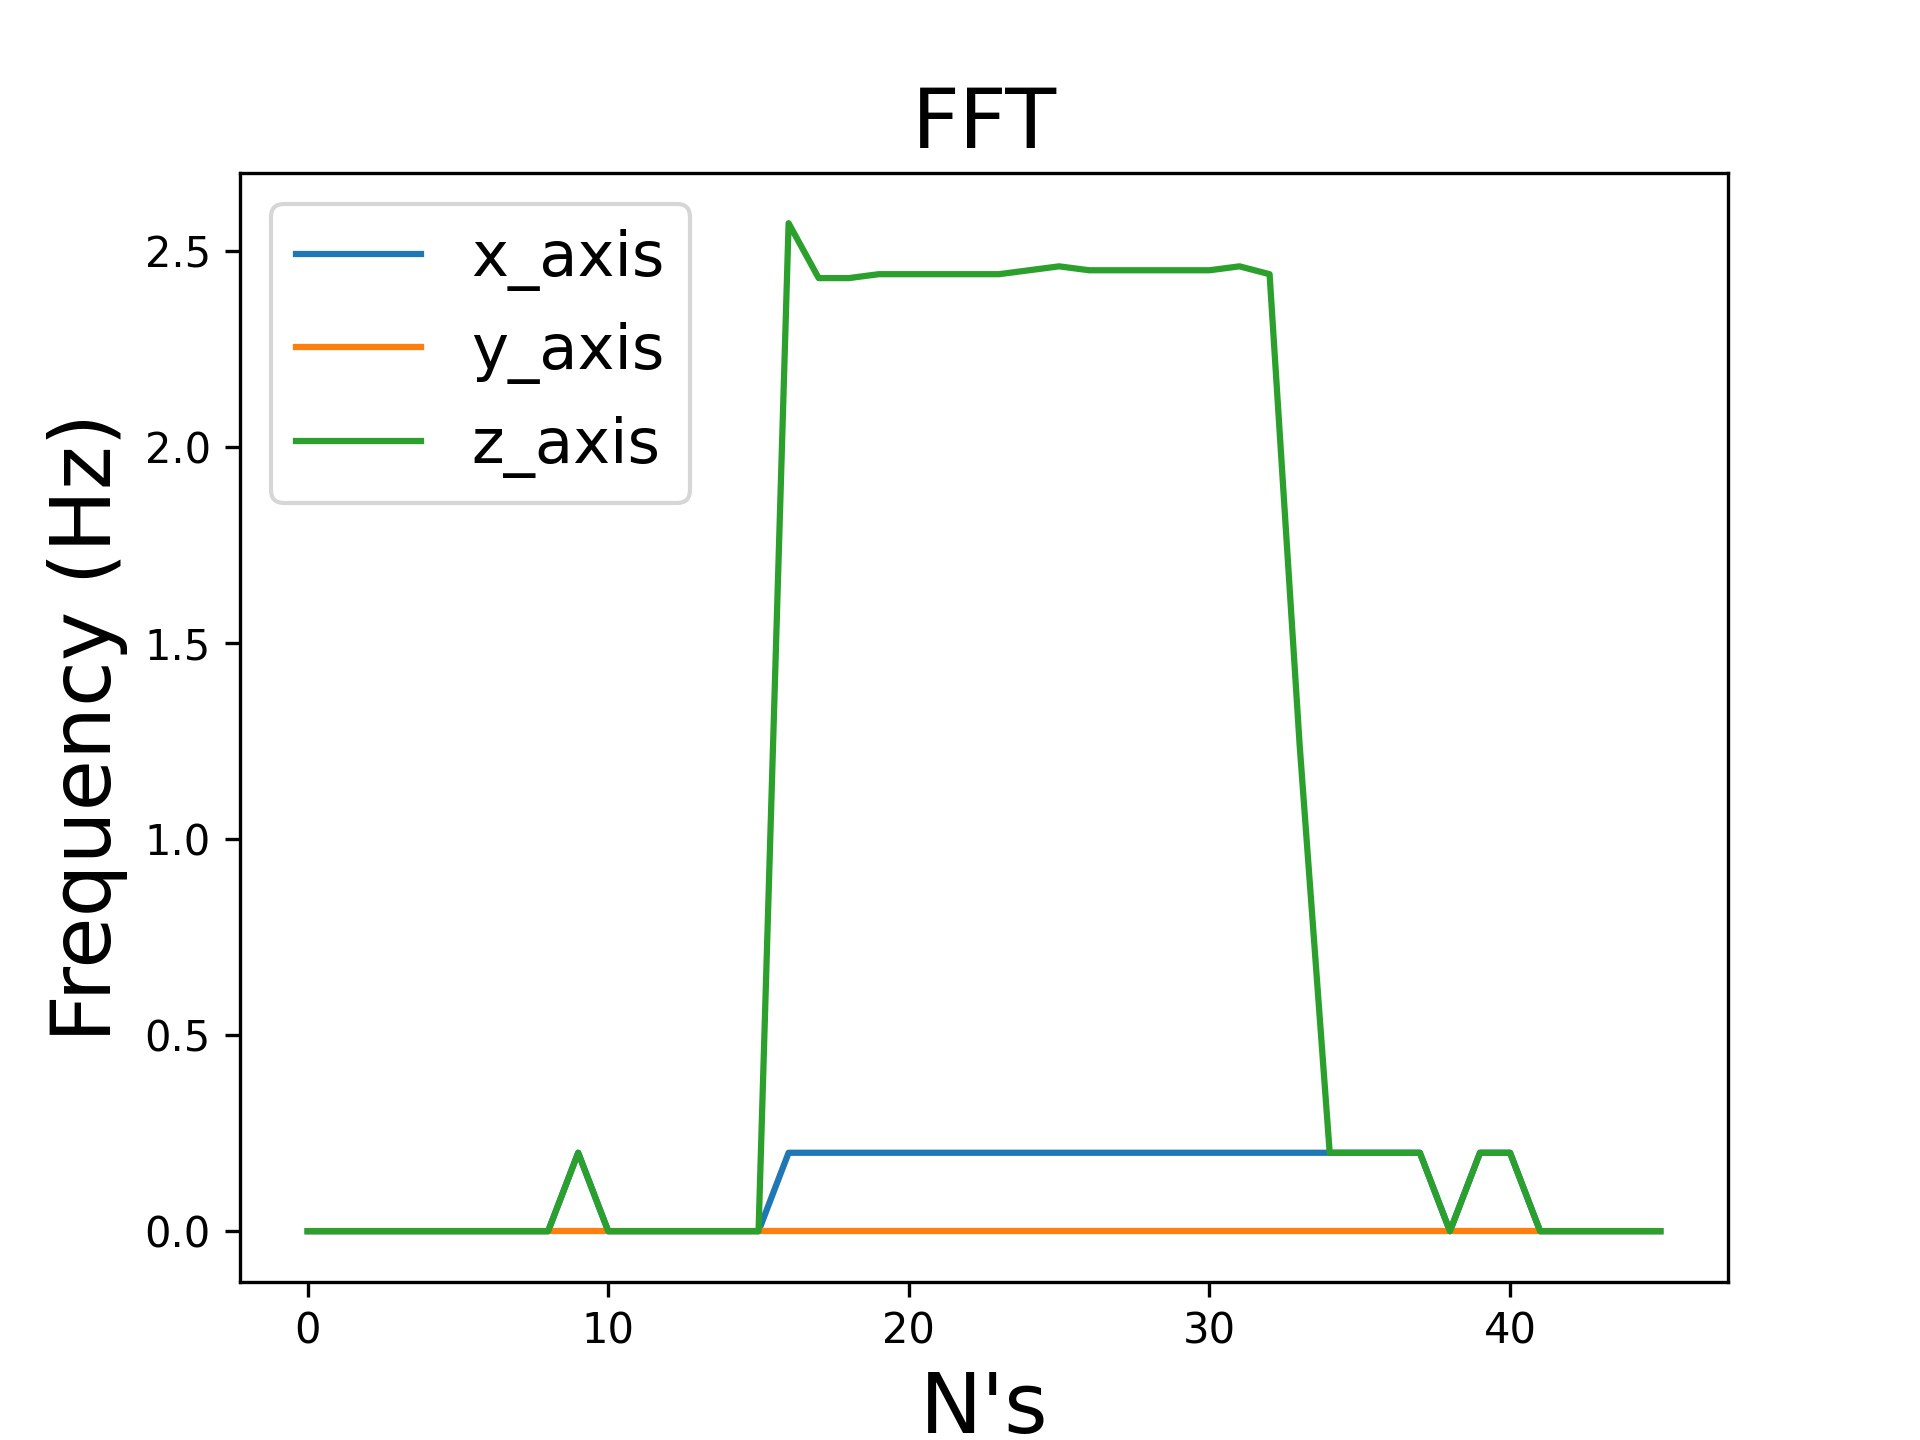
\includegraphics[width=.9\textwidth]{Sections/Prototype-Testing/PosterF.png}
	\label{proto1-test1-f}
\end{figure}

\subsubsection{Prototype 1: Test 2}
Test two removed the serial connection between the node device and the laptop and used the battery pack to power the device instead. The aim of this test was to achieve the same results as test one with a different input voltage and no serial connection for the node device. To initiate the test, the battery pack was switched on, and the reset button on the device was pushed, calibrating the accelerometer with the new reference voltage. This time only the receiver Python logging script was executed following the release of the beam. Once the beam reached its resting state the logging script was ended and the receiver Python plotting script was executed. The maximum acceleration and maximum frequency were plotted using pyplot and saved as PNG files. Figure \ref{beam-test-wireless} displays the node device on the beam with no physical connection to the laptop. 

\subsubsection{Prototype 1: Test 2 Results}
Figures \ref{proto1-test2-ma} and \ref{proto1-test2-f} show the maximum acceleration and maximum frequency from the serial connection between the gateway device and the laptop. These results show the same response as test one which verify the capability of the device running from the battery pack and successful calibration of the accelerometer when using a lower reference voltage of 3.0V. 

\begin{figure}[H]
	\centering
	\caption{Wireless Node in Beam Test}
	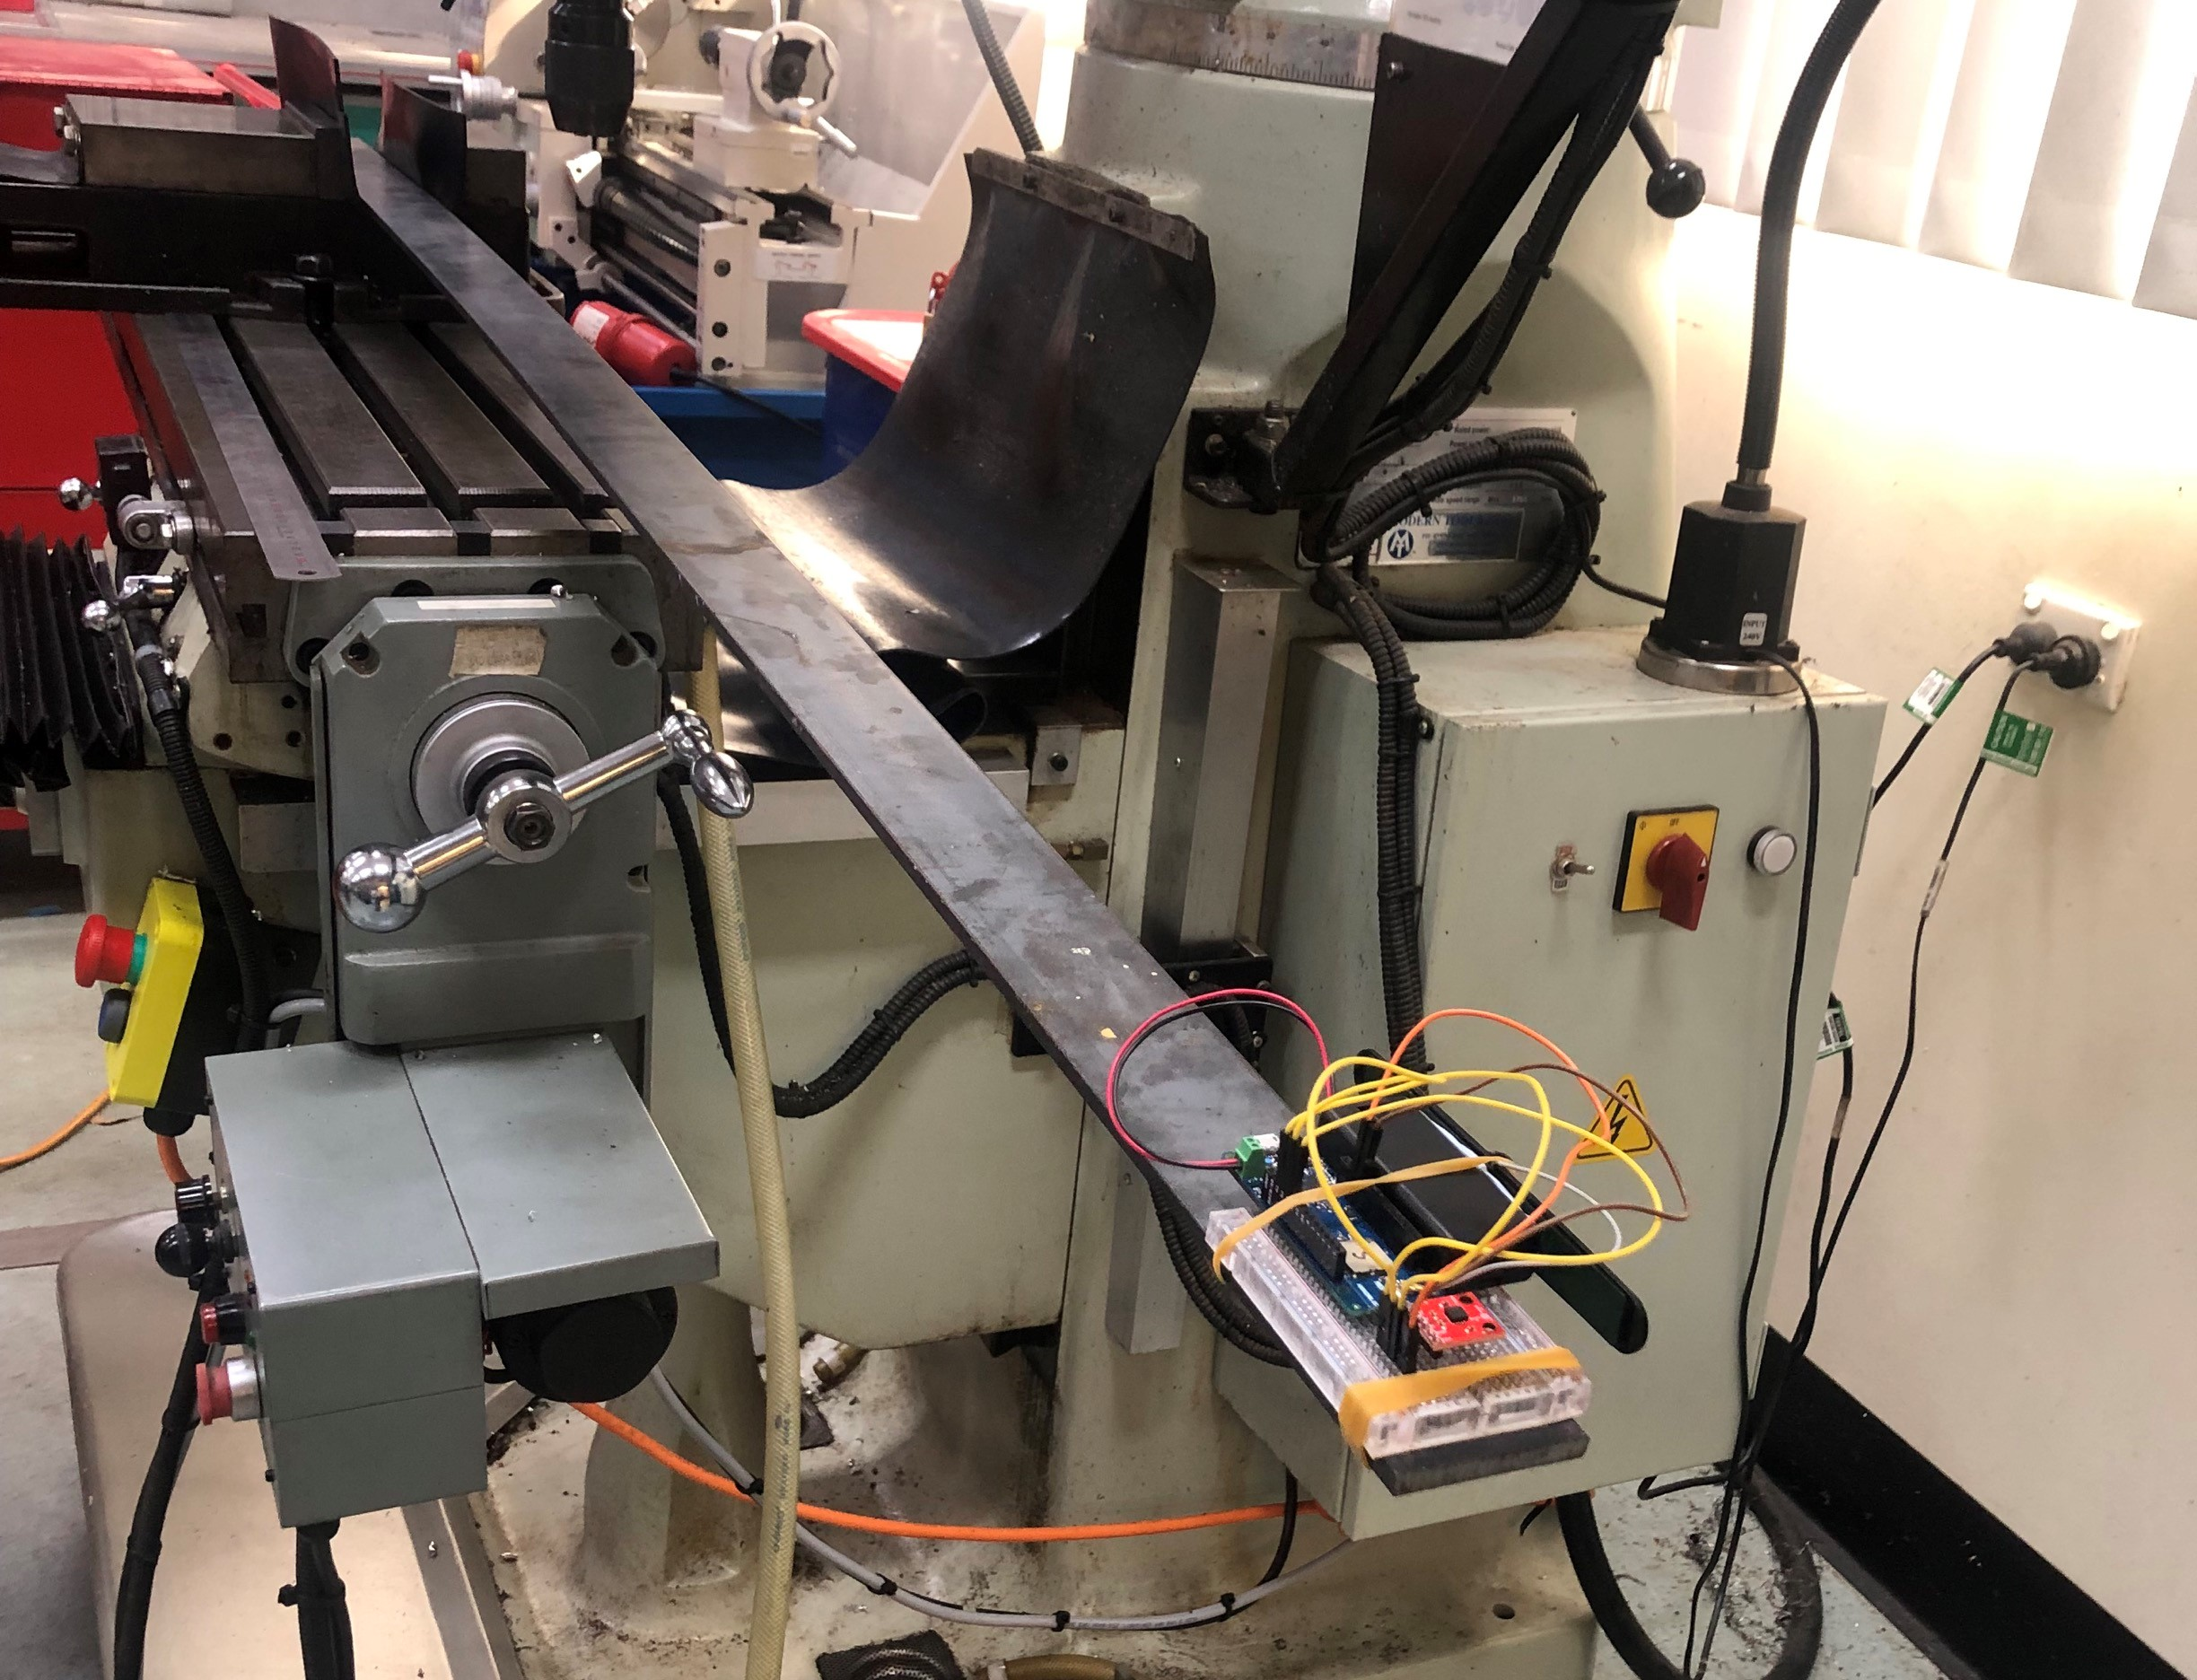
\includegraphics[width=.8\textwidth]{Sections/Prototype-Testing/beam-test-wireless.png}
	\label{beam-test-wireless}
\end{figure}

\begin{figure}[H]
	\centering
	\caption{Prototype 1: Test 2 Maximum Acceleration}
	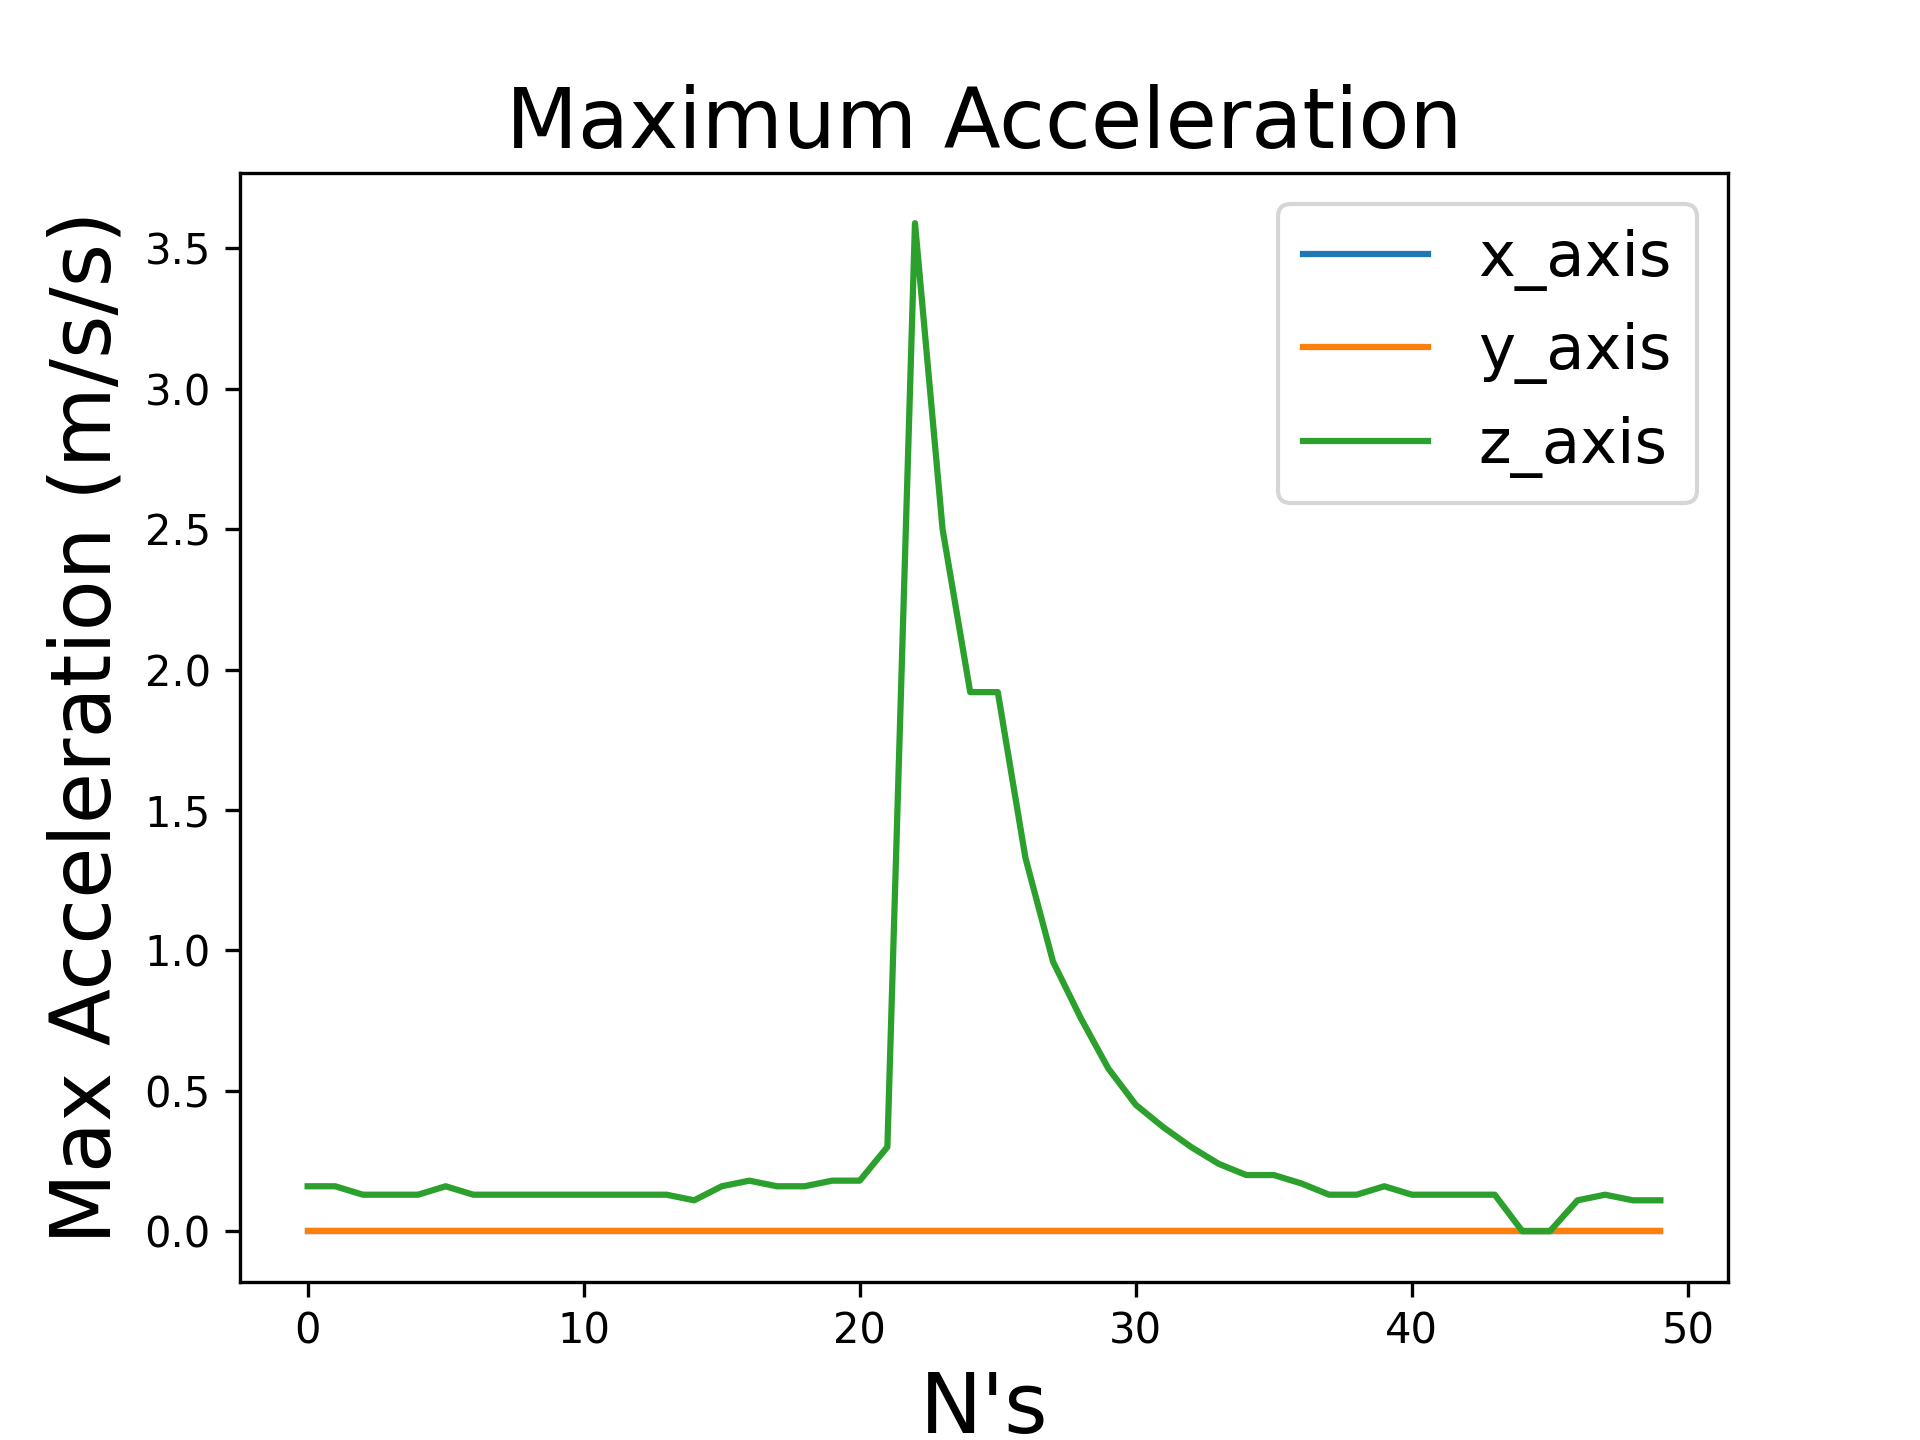
\includegraphics[width=.9\textwidth]{Sections/Prototype-Testing/test2-ma.png}
	\label{proto1-test2-ma}
\end{figure}

\begin{figure}[H]
	\centering
	\caption{Prototype 1: Test 2 Maximum Frequency}
	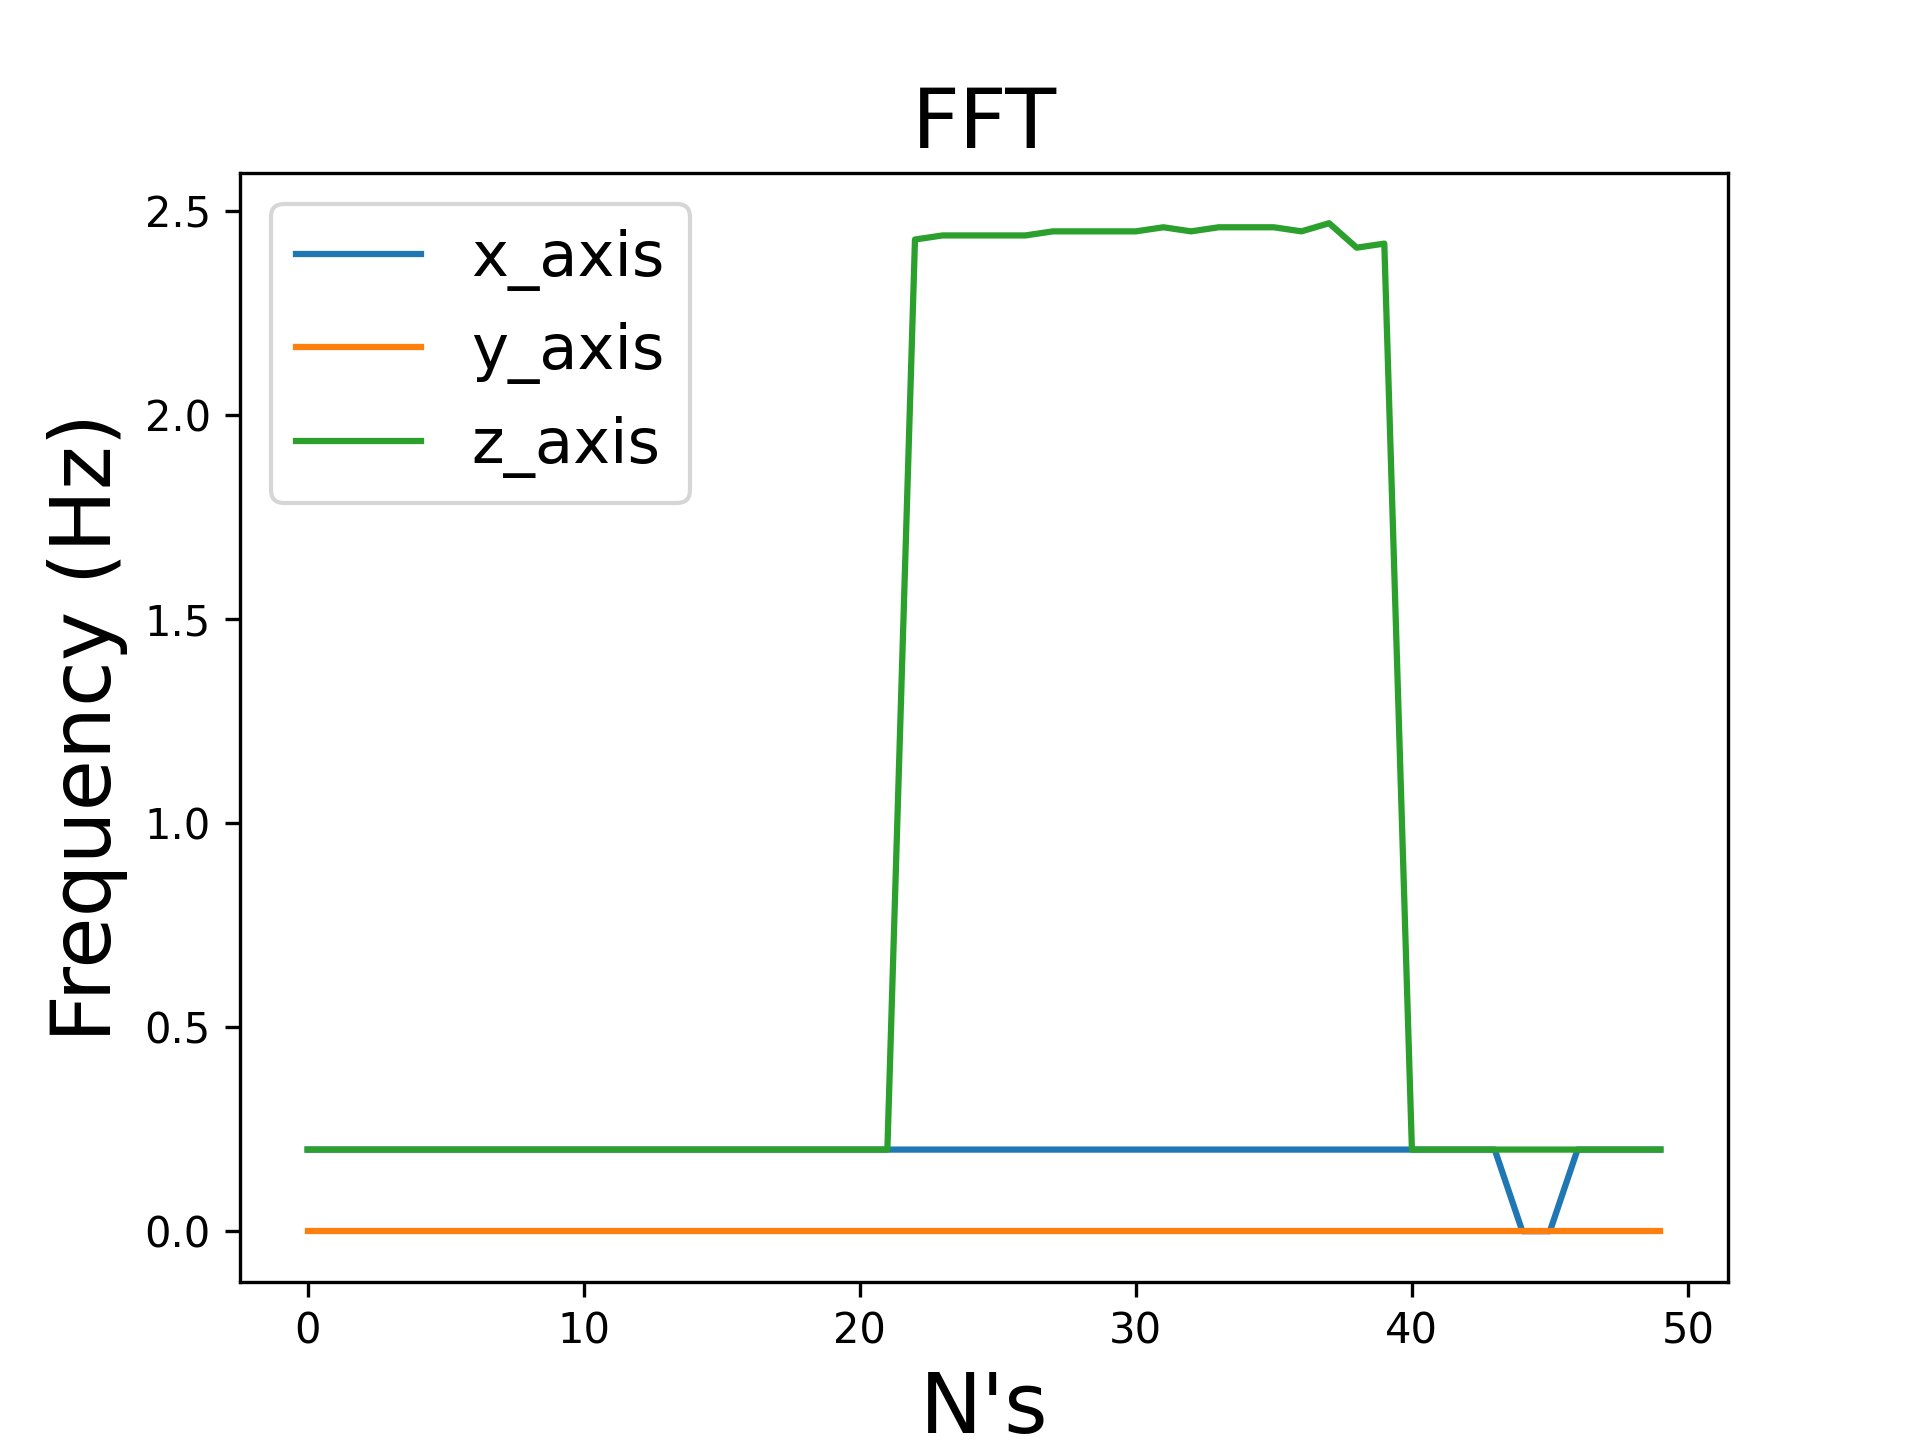
\includegraphics[width=.9\textwidth]{Sections/Prototype-Testing/test2-f.png}
	\label{proto1-test2-f}
\end{figure}

\subsubsection{Prototype 1: Test 3}
The purpose of test three was to test the range of the communication between the two devices. To do this one participant stayed in the laboratory and the other carried the laptop away with the gateway node which was still connected serially. A Microsoft Teams call was used to communicate between the two participants during this test. The beam was continuously pushed down and the data was observed on the Arduino IDE's live serial plotter. The test was ended once the gateway node was unable to receive LoRa packets and the location was recorded. 

\subsubsection{Prototype 1: Test 3 Results}
Figure \ref{proto1-test3-range} shows the maximum range of successful communication between the two devices. The range was measured between the mechanical engineering laboratory and the start of the Griffith footbridge, reaching a distance of approximately 200m. 

\begin{figure}[H]
	\centering
	\caption{Prototype 1: Test 3 Range \cite{test3-range}}
	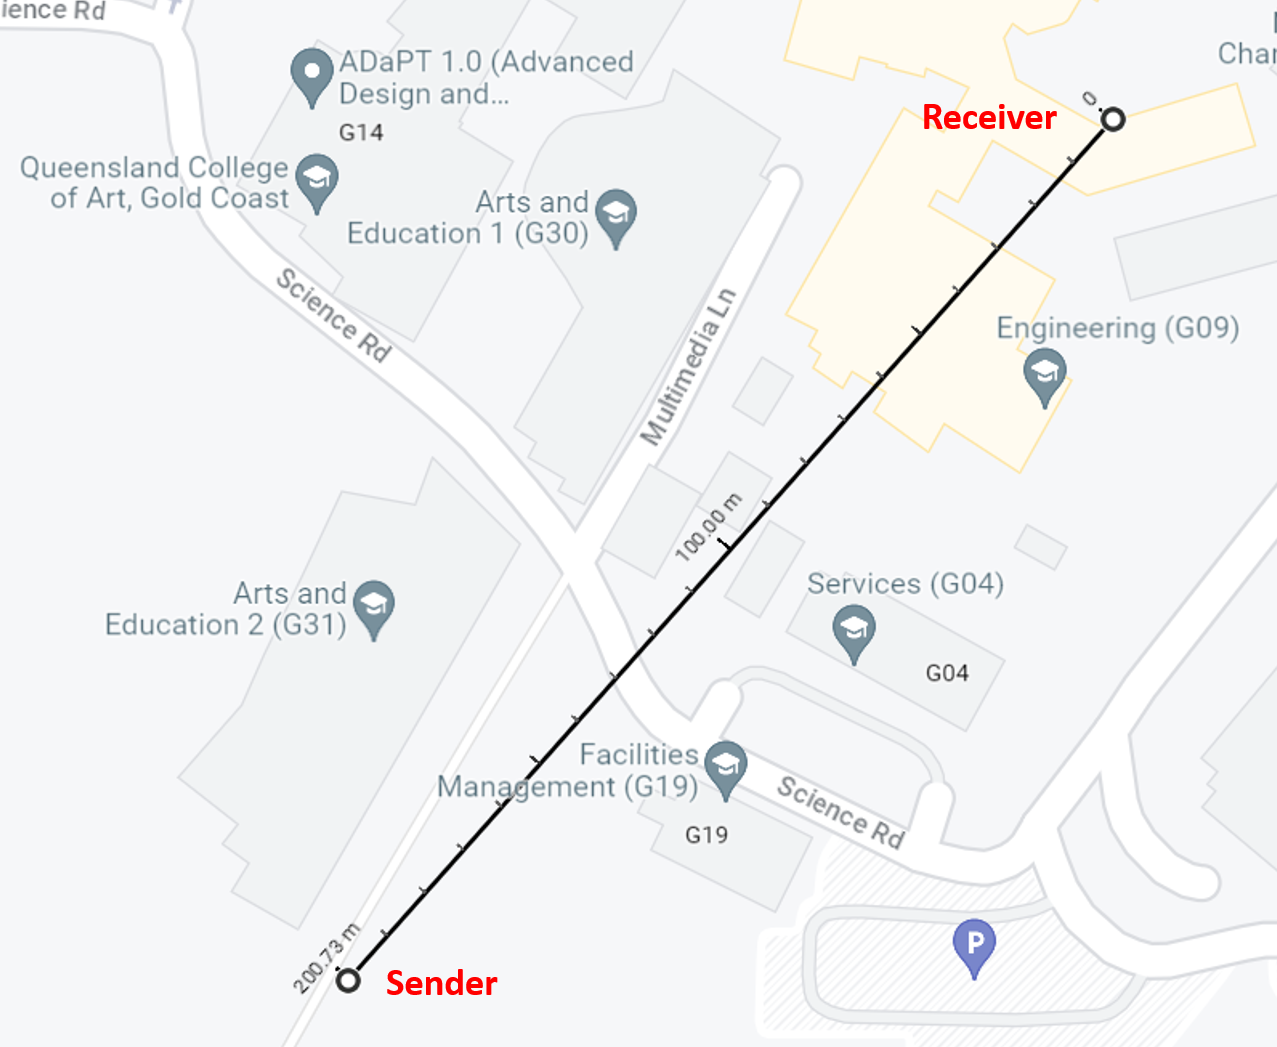
\includegraphics[width=\textwidth]{Sections/Prototype-Testing/test3-range-label.png}
	\label{proto1-test3-range}
\end{figure}

\subsection{Prototype 2: Bridge Test}
The purpose of the bridge test was to test a full deployment of IoT architecture for structural health monitoring and to verify the first mode flexural frequency stated in the Griffith footbridge documentation. This test involved installing the enclosure behind the hand rail of the footbridge and setting up a base station for data collection. The base station was placed 25m away from the node device and consisted of a power generator, laptop and LoRaWAN gateway. Similar to the prototype one testing, the noise threshold values were fine tuned over the course of several experiments. The Arduino IoT Cloud dashboard was used to monitor the data live feed, figure \ref{dashboard}, and the TNN live data page, figure \ref{tnn-live}, was used to observe incoming LoRa packets. The base station can be seen in figure \ref{base-station} and the enclosure installation can be seen in figure \ref{enclosure-integration}. The testing was conducted between 4:00 pm and 6:00pm and the bridge was subjected to moderate pedestrian load from the university and a nearby school. 

\begin{figure}[H]
	\centering
	\caption{Base Station Setup}
	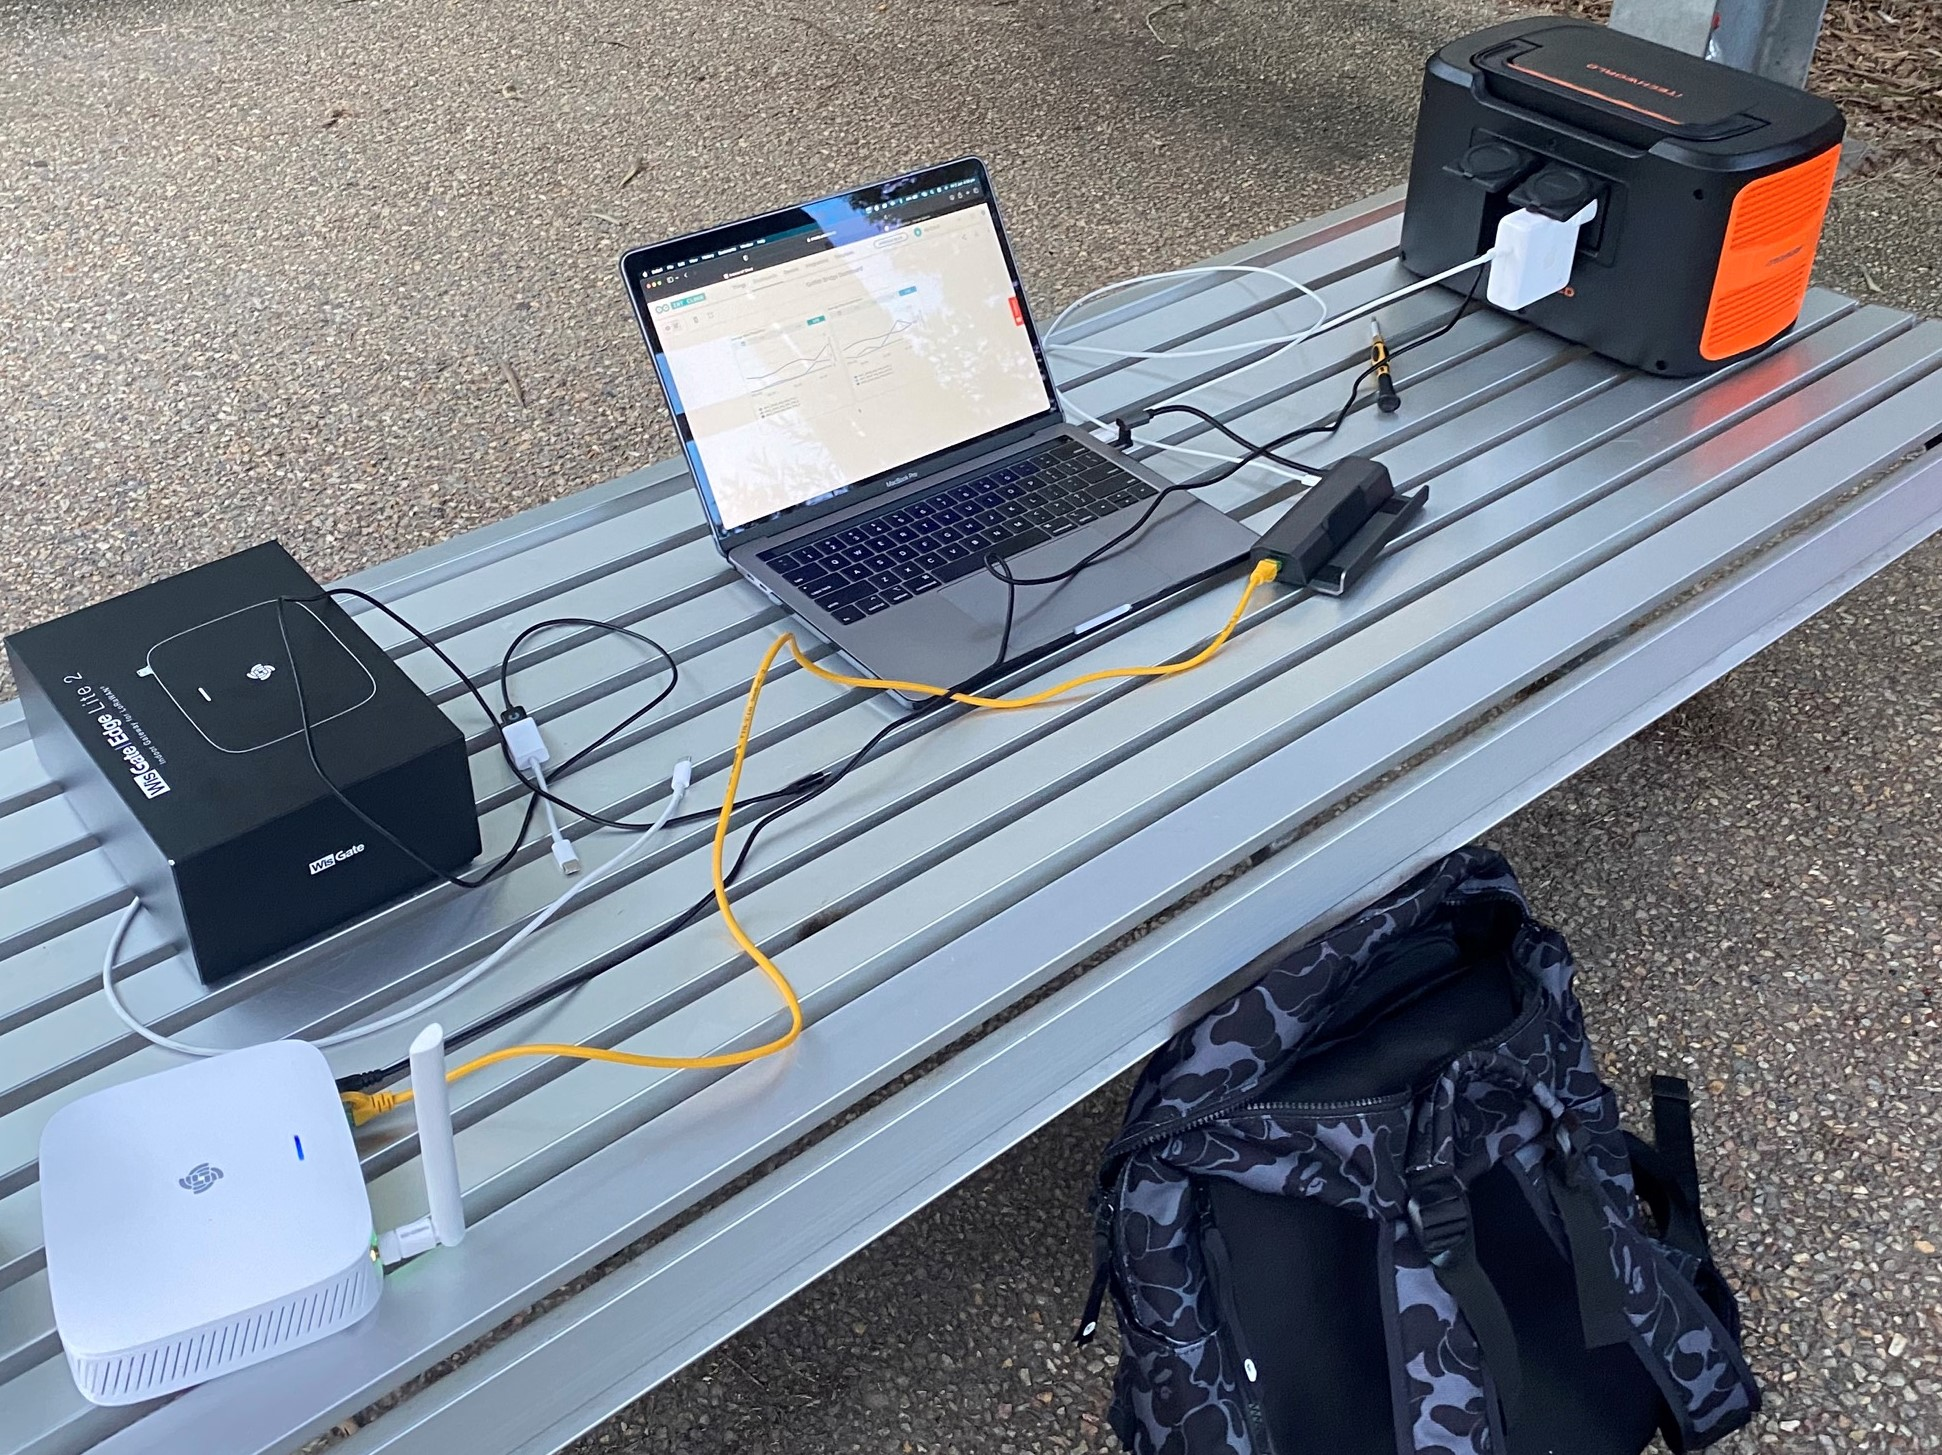
\includegraphics[width=\textwidth]{Sections/Prototype-Testing/base-station.png}
	\label{base-station}
\end{figure}

\subsubsection{Prototype 2: Test 1}
Test one was conducted over a thirty minute period with noise threshold values 0.05 for the x-axis, 0.05 for the y-axis and 0.03 for the z-axis. The purpose of this test was to determine if these noise threshold values were suitable for achieving the expected frequency response of the bridge and to observe the signal strength over time. It was discovered in this test that the enclosure lid was too thick and prevented packet transmission so it was removed for testing. Packets were sent from the node device every sixty seconds and these points were plotted in the Arduino IoT Cloud dashboard. Two participants were required for this experiment, one to monitor the incoming packets on the TNN live data page at the base station, and one to safeguard the enclosure on the bridge. Figure \ref{bridge-axis} displays the orientation of each axis with respect to the enclosure placement on the bridge. 

\begin{figure}[H]
	\centering
	\caption{Prototype 2: Test 1 Enclosure Bridge Axis}
	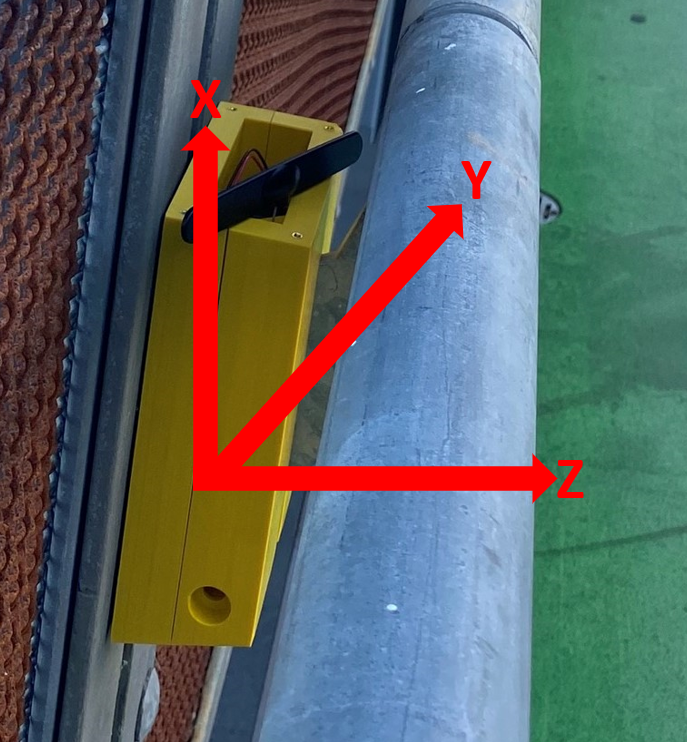
\includegraphics[width=.7\textwidth]{Sections/Prototype-Testing/bridge-axis.png}
	\label{bridge-axis}
\end{figure}

\subsubsection{Prototype 2: Test 1 Results}
Figures \ref{proto2-test1-a} and \ref{proto2-test1-f} show the maximum average acceleration and maximum average frequency over a thirty minute period. Figures \ref{proto2-test1-snr} and \ref{proto2-test1-rssi} show the SNR and RSSI of the signal over the testing duration. Unlike the beam experiment, the x-axis was designed to represent the vertical frequency component of the bridge and so the noise threshold value of 0.03 was determined to be too low. The peaks in the acceleration and frequency values are representative of the pedestrian load during testing.\\\\ The SNR during this test fluctuated between 10 dB to 15 dB which is characteristic of a good connection. Positive SNR for LoRaWAN indicates that the signal can be successfully demodulated from the noise \cite{TNN-SNR-RSSI}. LoRa SNR usually lies between -20 dB and 10 dB, with SNR closer to 10 dB characterising a good connection \cite{LoRa-SNR-RSSI}. The RSSI values  averaged values between -70 dBm and -85 dBm. RSSI values for LoRa are more resilient than other communication technologies such as 2G and 3G Wi-Fi which 
list the range of -70 dBm to -85 dBm as a strong signal with good data speeds \cite{WIFI-RSSI}. The signal drops to -110 dBm on the fourth packet which is very low, however LoRa is resilient enough to transmit packages as low as -120 dBm, so the signal is not fully disconnected at this point. 

\begin{figure}[H]
	\centering
	\caption{Prototype 2: Test 1 Maximum Average Acceleration}
	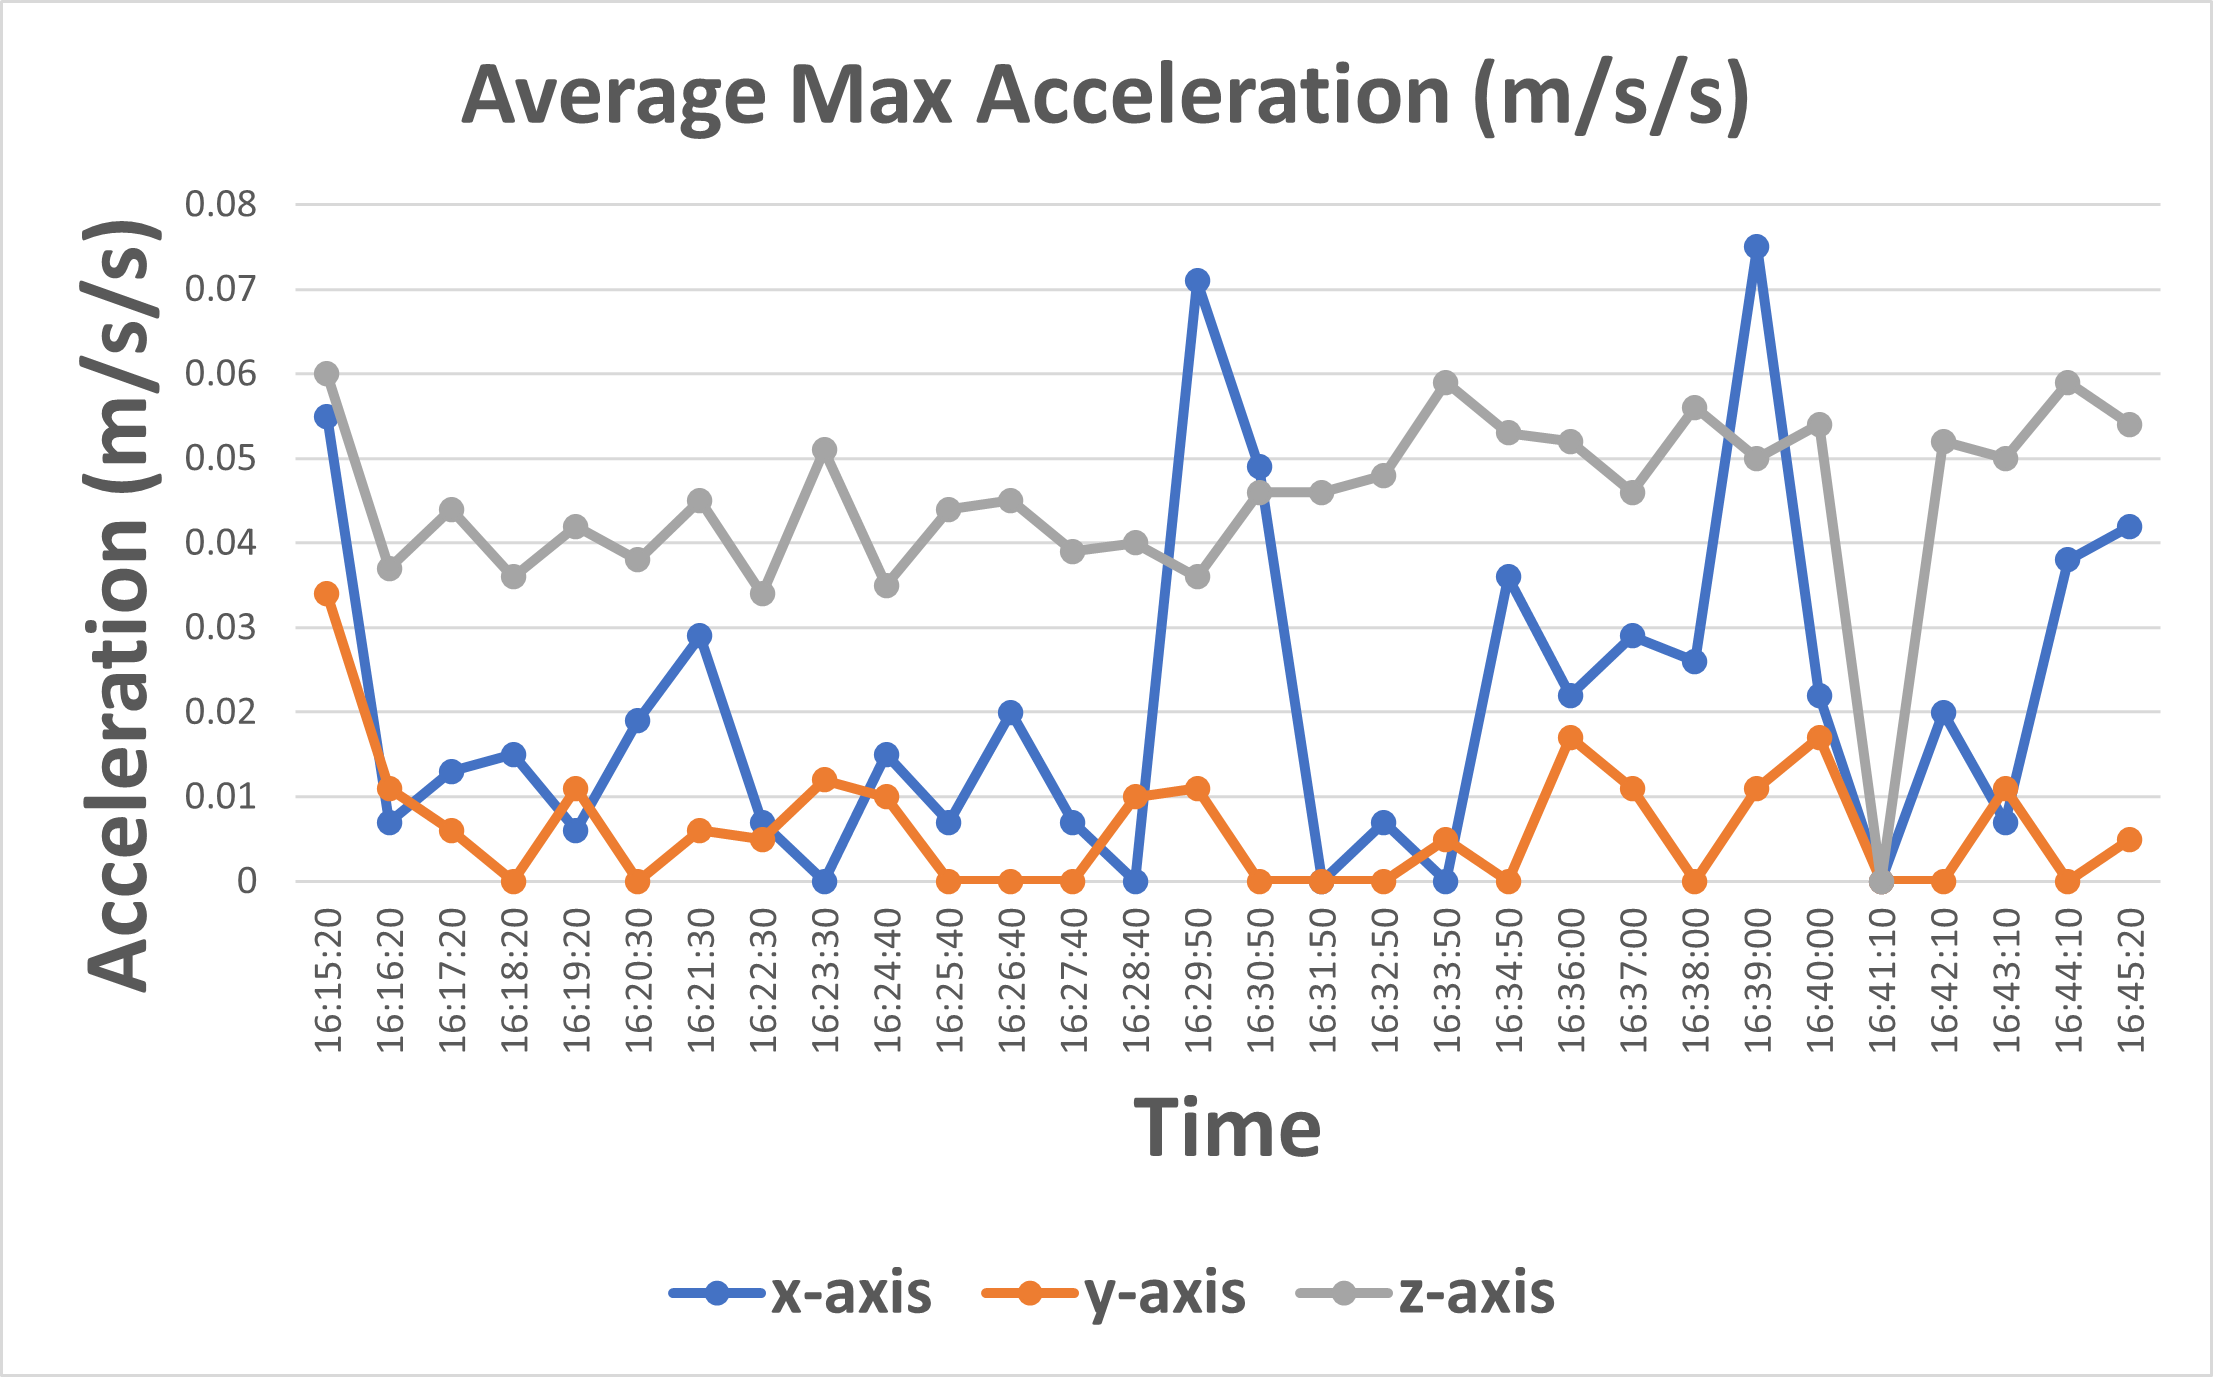
\includegraphics[width=\textwidth]{Sections/Prototype-Testing/proto2-test1-a.png}
	\label{proto2-test1-a}
\end{figure}

\begin{figure}[H]
	\centering
	\caption{Prototype 2: Test 1 Maximum Average Frequency}
	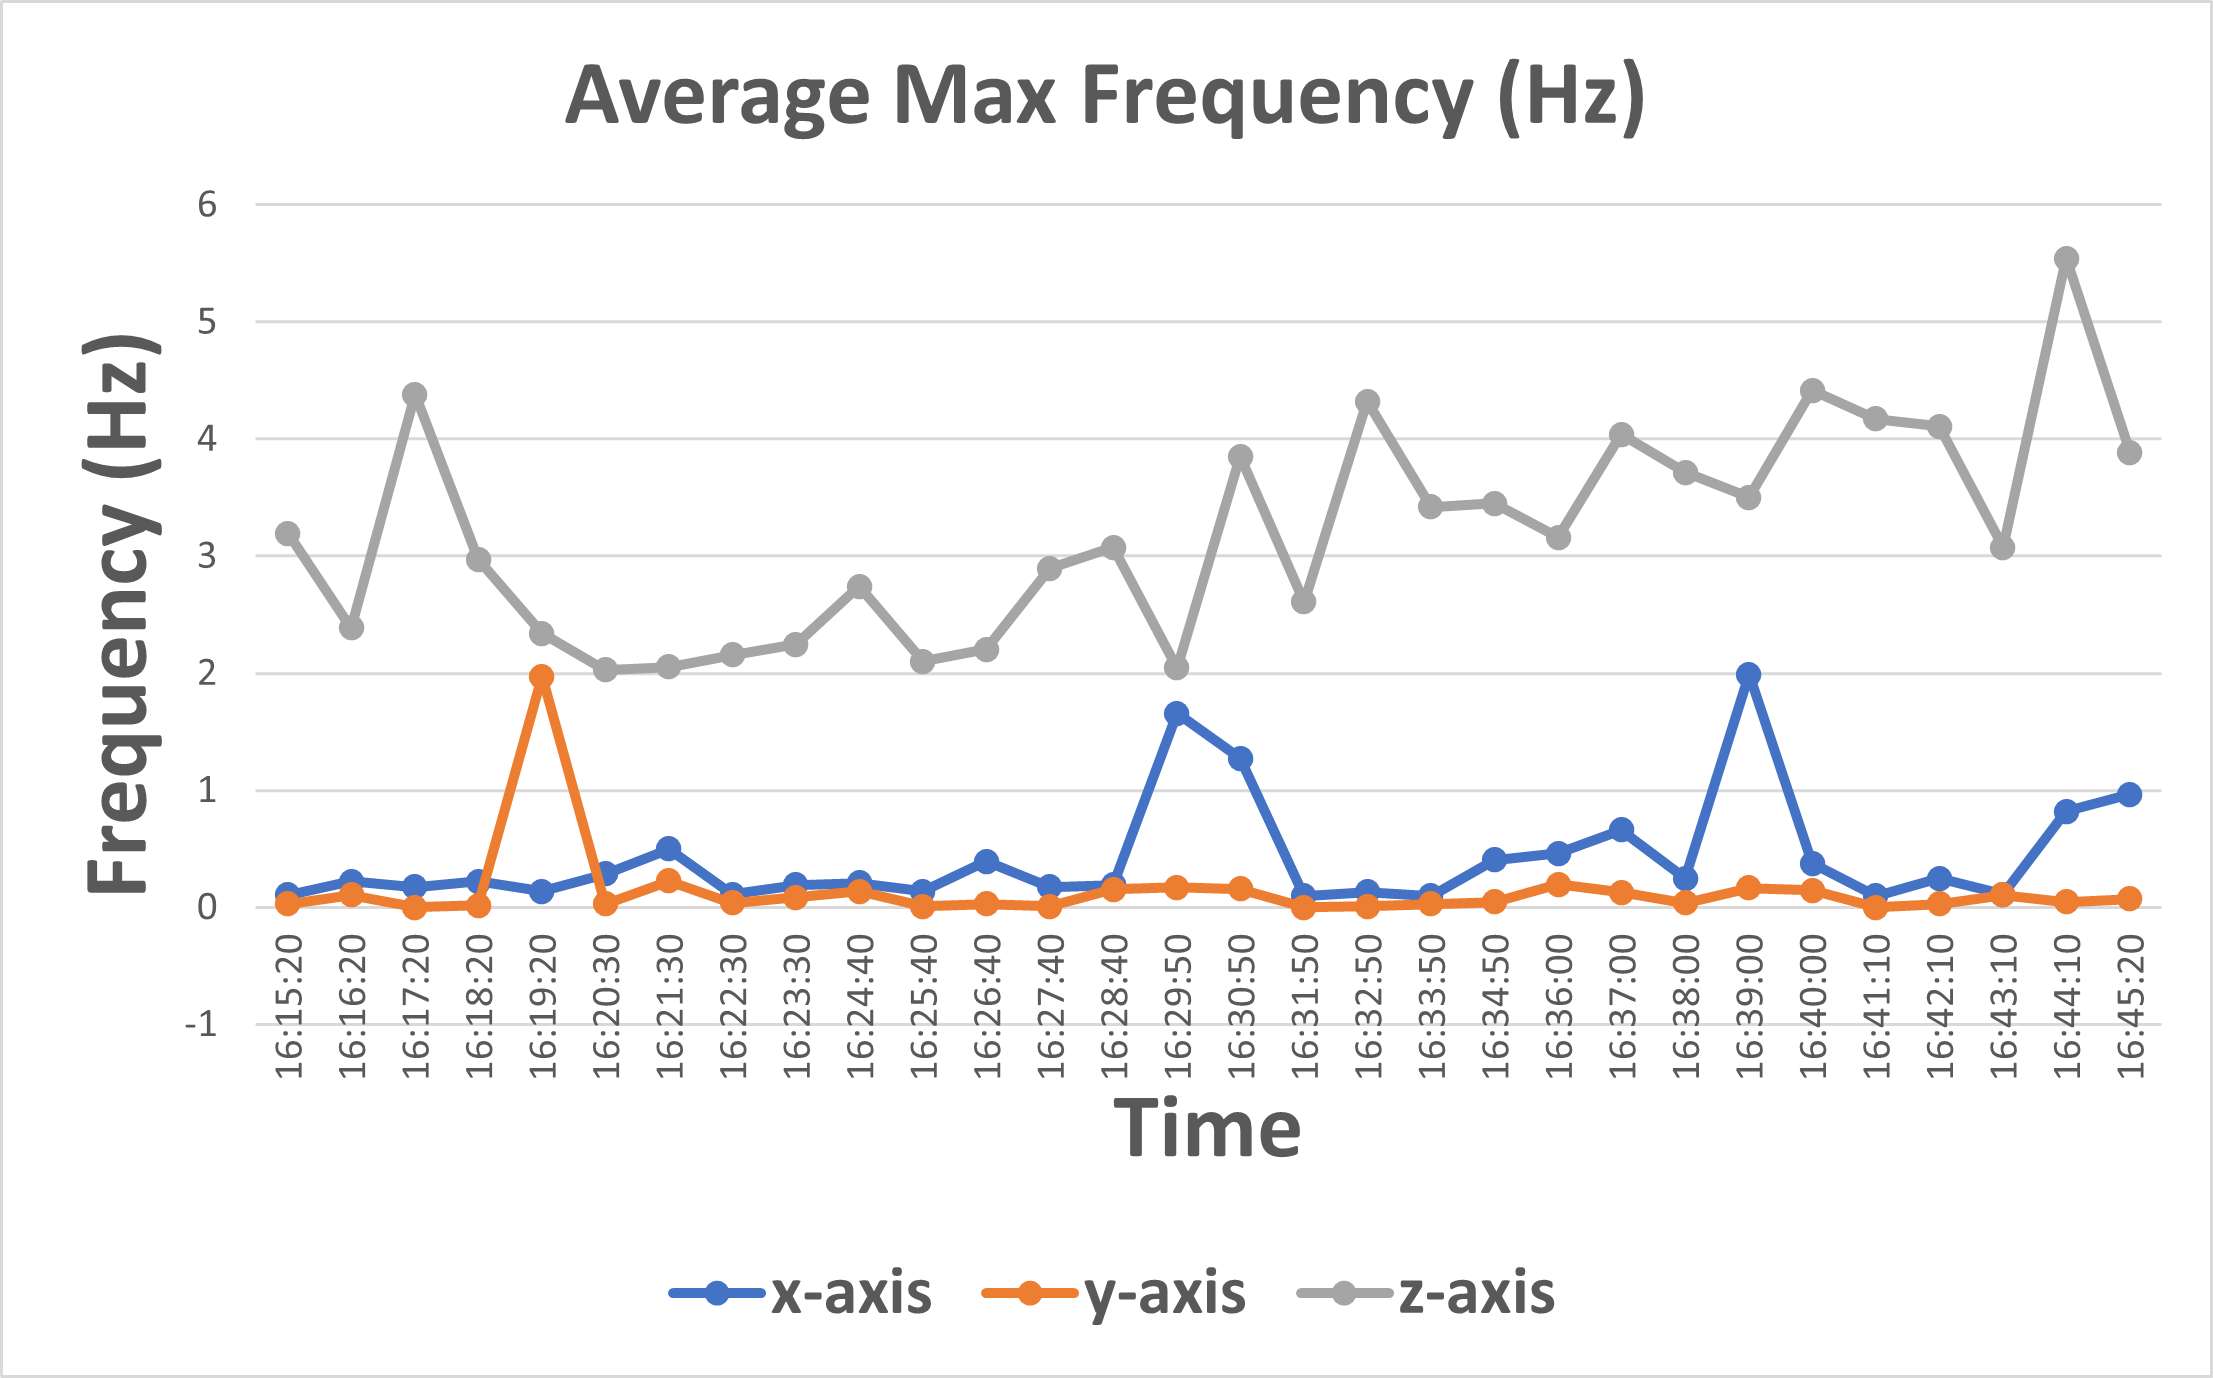
\includegraphics[width=\textwidth]{Sections/Prototype-Testing/proto2-test1-f.png}
	\label{proto2-test1-f}
\end{figure}

\begin{figure}[H]
	\centering
	\caption{Prototype 2: Test 1 SNR}
	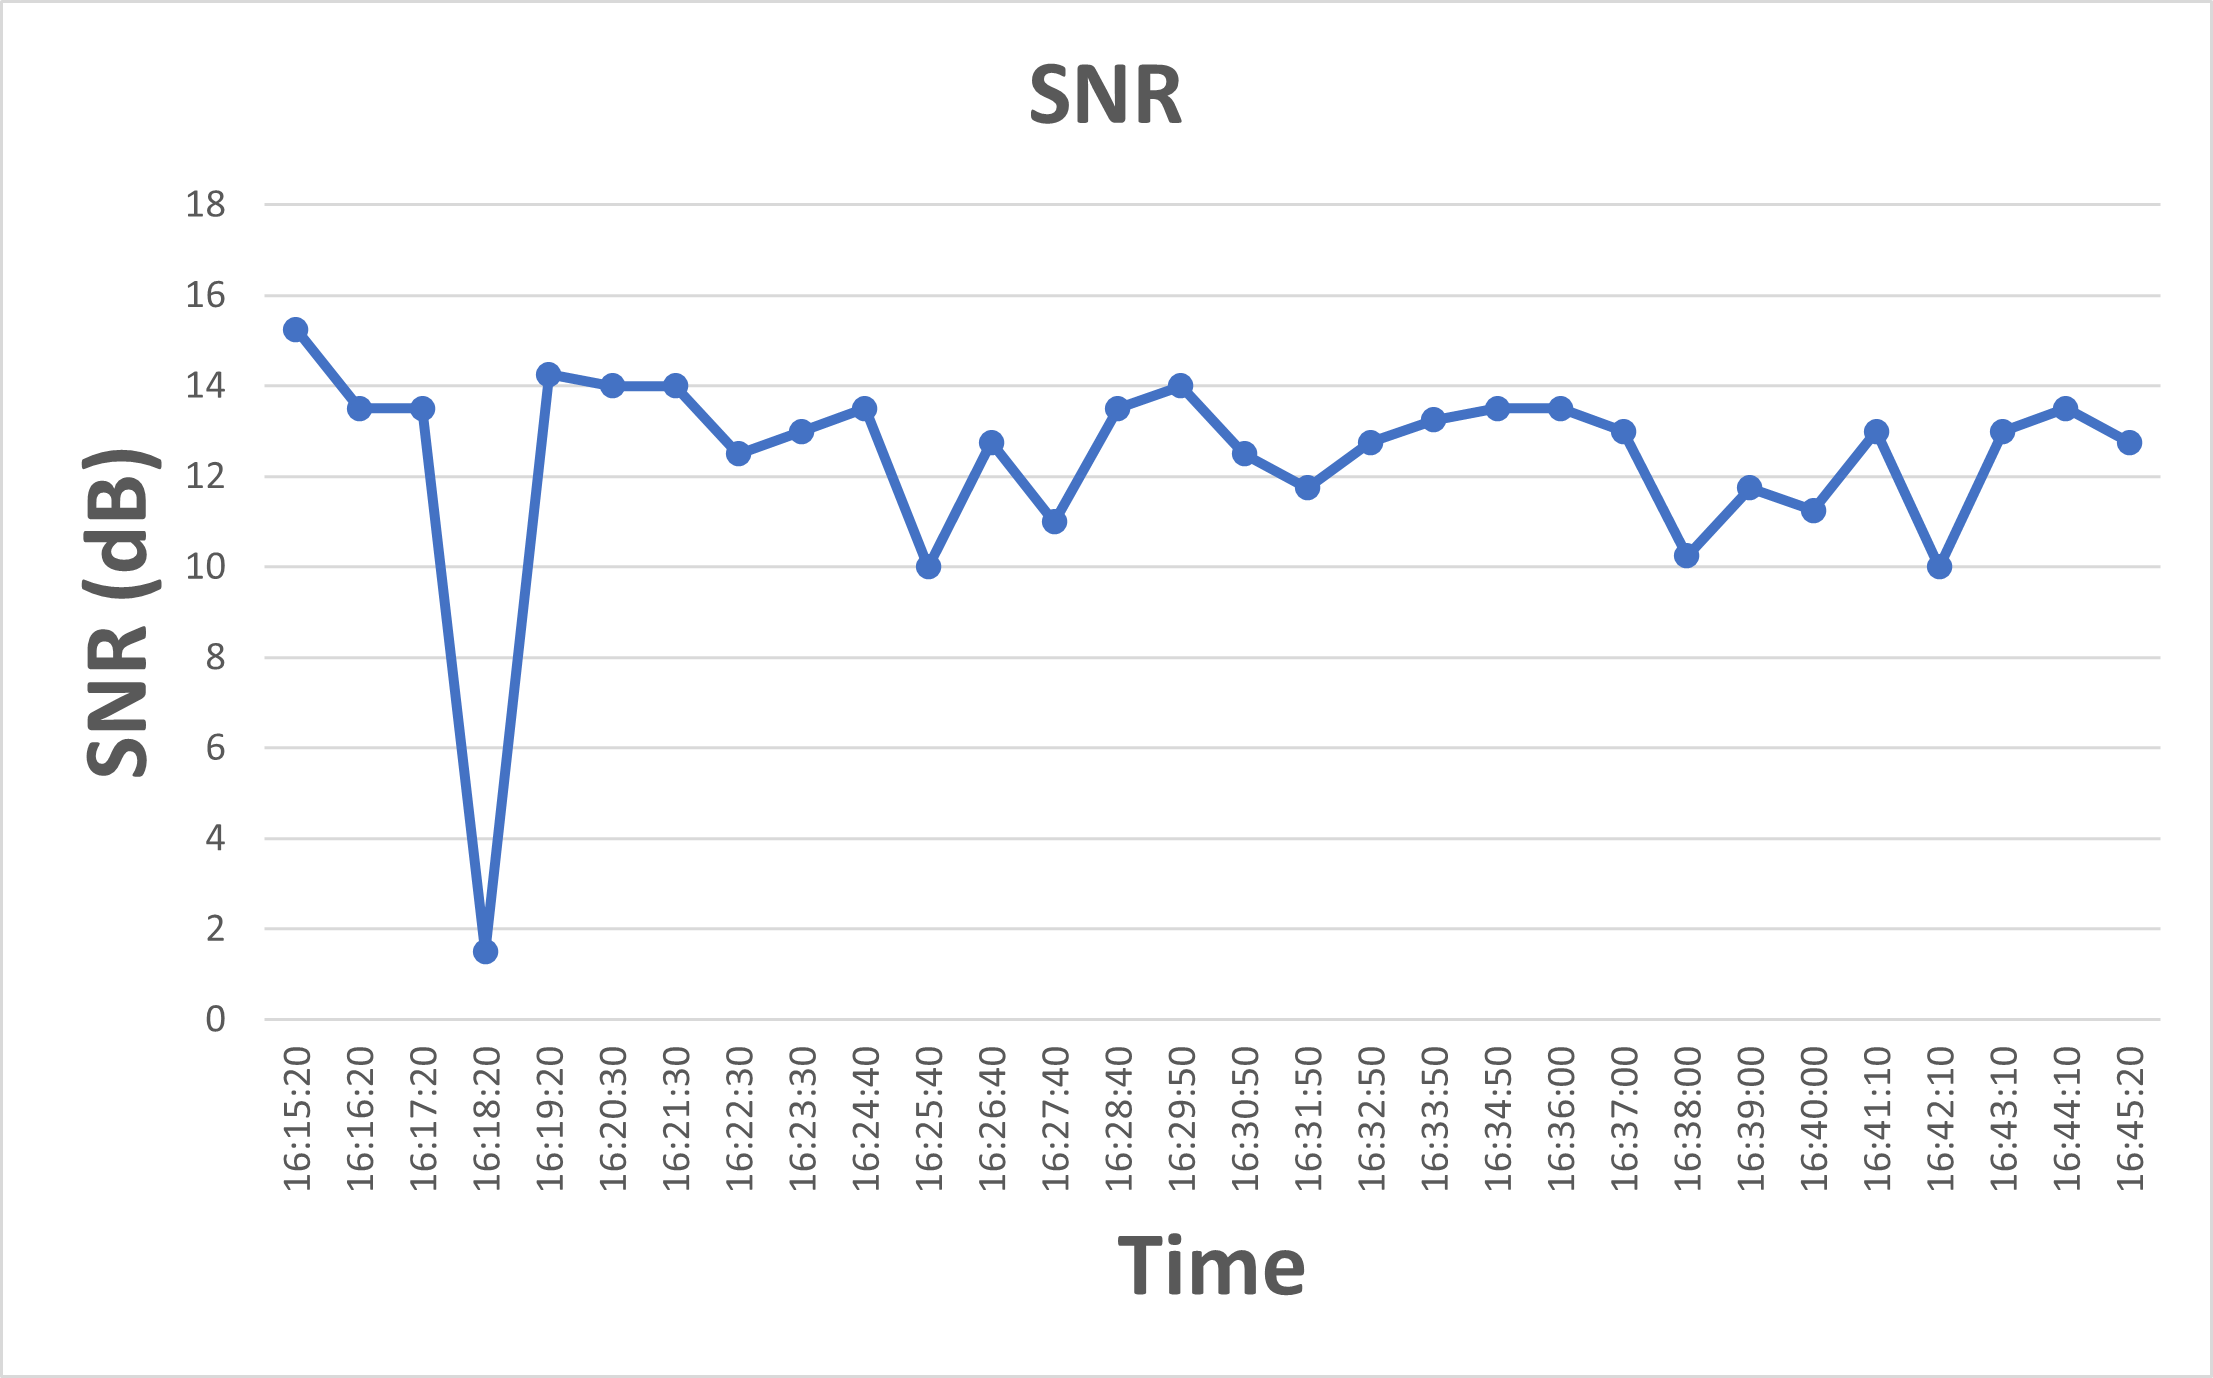
\includegraphics[width=\textwidth]{Sections/Prototype-Testing/proto2-test1-snr.png}
	\label{proto2-test1-snr}
\end{figure}

\begin{figure}[H]
	\centering
	\caption{Prototype 2: Test 1 RSSI}
	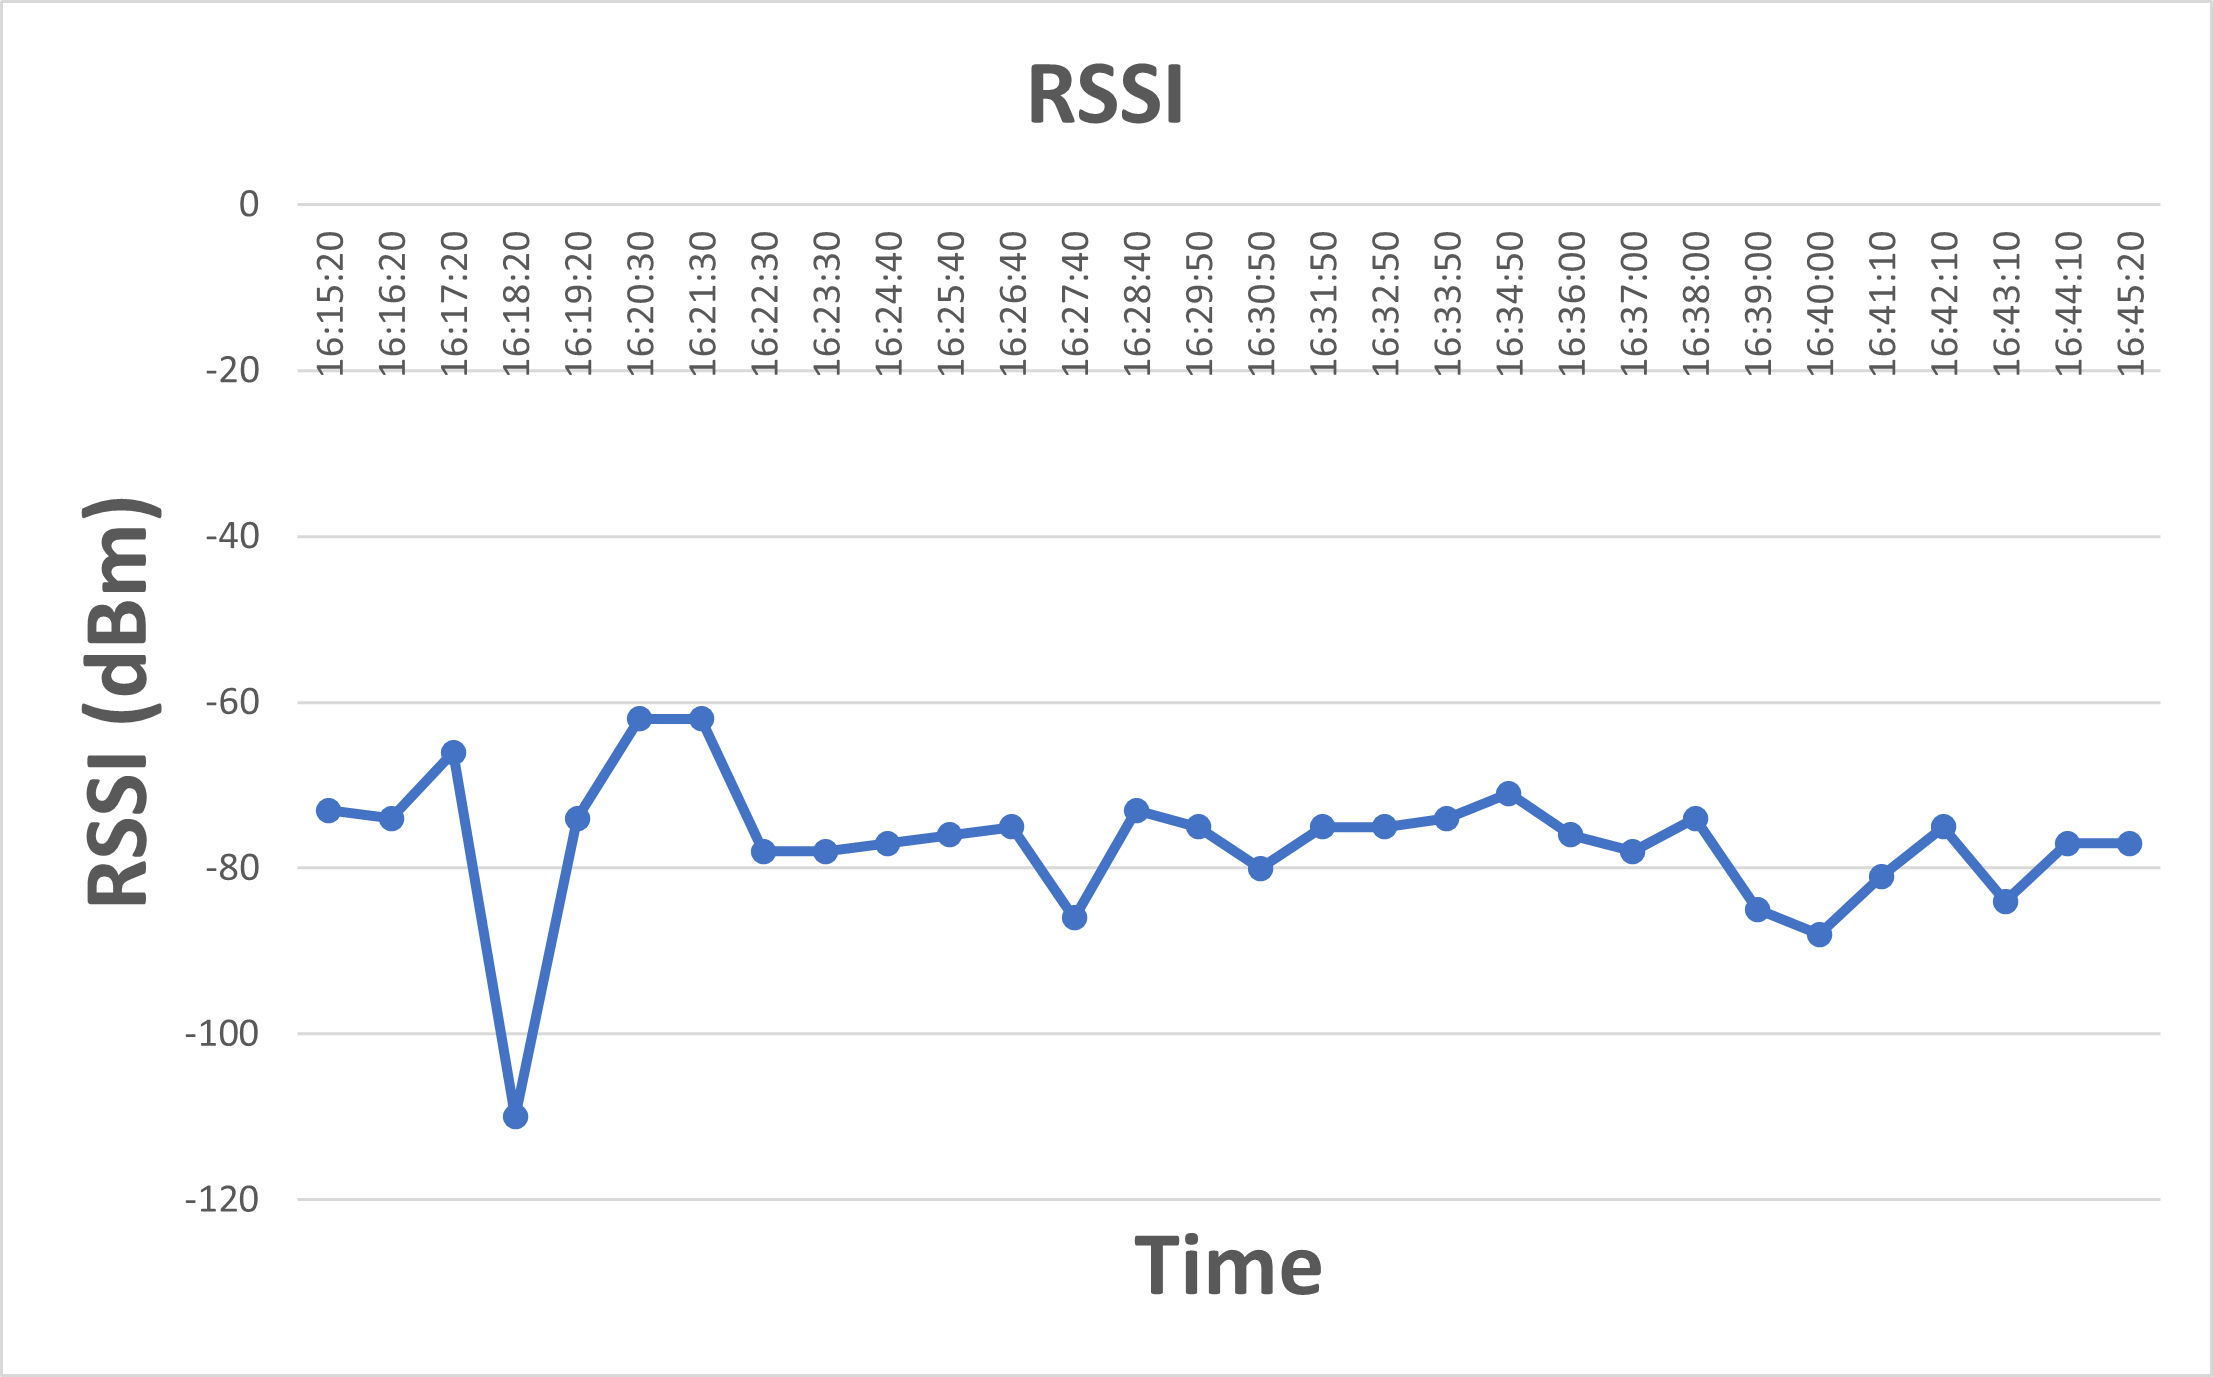
\includegraphics[width=\textwidth]{Sections/Prototype-Testing/proto2-test1-rssi.png}
	\label{proto2-test1-rssi}
\end{figure}

\subsubsection{Prototype 2: Test 2}
Test two was conducted over a thirty minute period with the same noise thresholds as test one. This time, the enclosure was removed from the rail and placed flat on the floor of the bridge. This was done to gain more context about the results from experiment one and insight for the noise threshold values used in test three. Figure \ref{bridge-ground} shows the enclosure placement for this test. Packets were again transmitted every sixty seconds and the values were observed in real time on the Arduino IoT Cloud dashboard. One participant was assigned to monitoring the incoming packets on the TNN live data page at the base station, and one to watch over the enclosure on the bridge. Special attention was required for this test since the enclosure was placed flat on the ground and was at risk of pedestrian interference. 

\begin{figure}[H]
	\centering
	\caption{Prototype 2: Test 2 Enclosure Placement}
	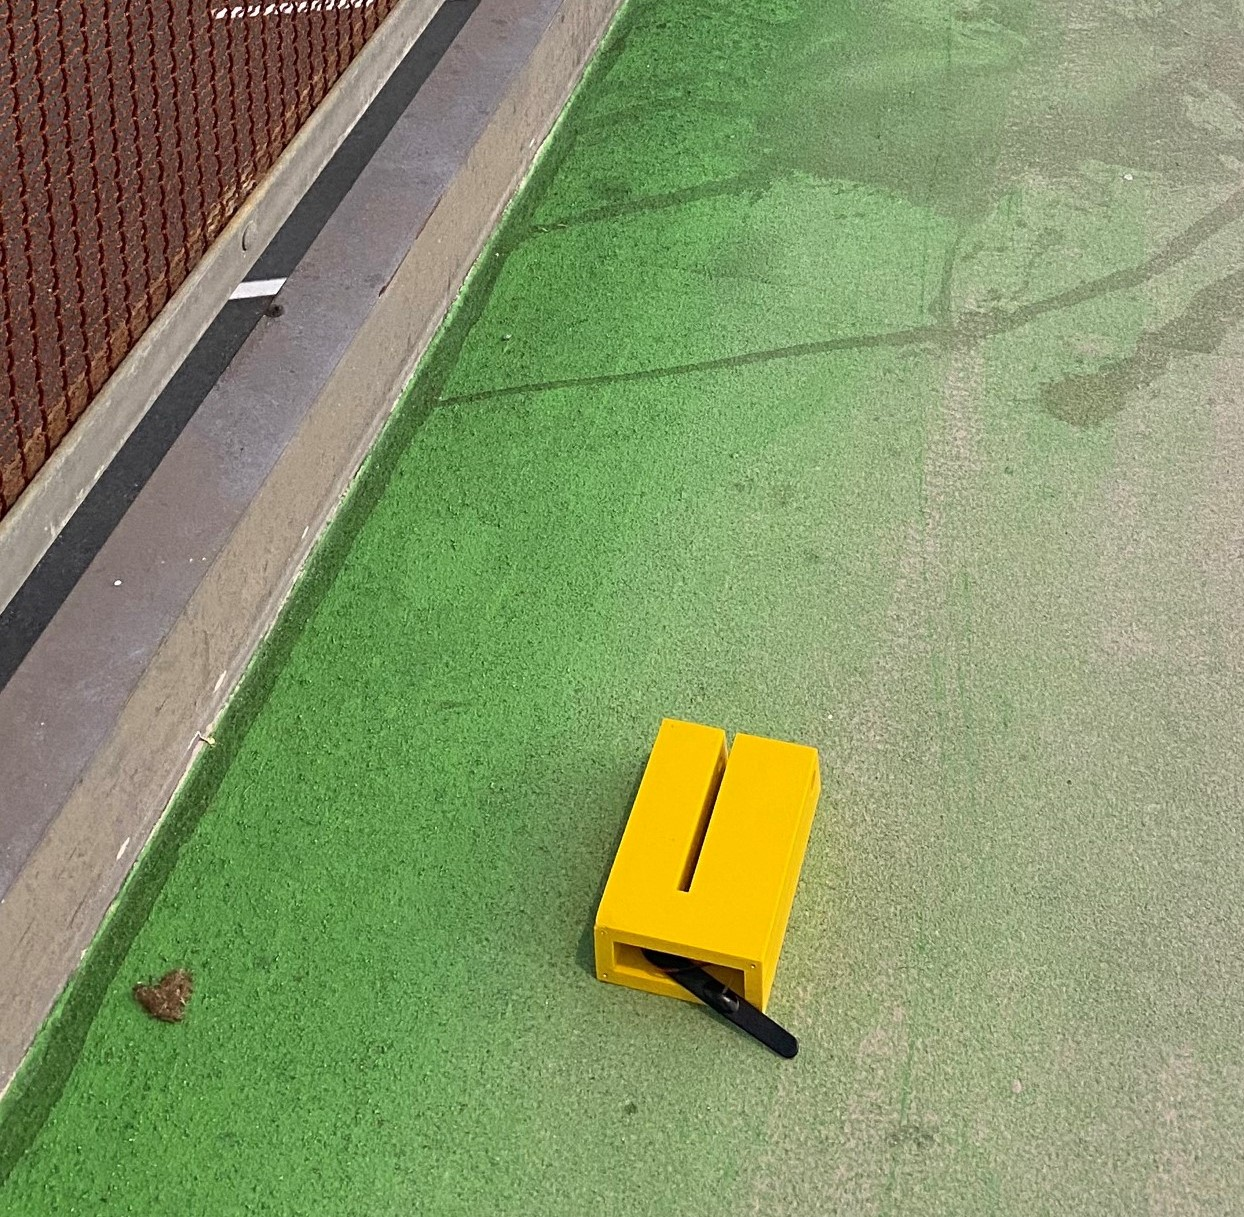
\includegraphics[width=0.8\textwidth]{Sections/Prototype-Testing/bridge-ground.png}
	\label{bridge-ground}
\end{figure}

\subsubsection{Prototype 2: Test 2 Results}
At the conclusion of test one, it was uncertain as to whether the lack of x-axis frequency was truly due to the lower noise threshold or if the z-axis was actually the result of the side of the bridge absorbing frequency components of the x-axis. To resolve this uncertainty the enclosure was placed flat on the bridge, making the z-axis representative of the vertical frequency component (test one x-axis). Since the noise thresholds were unchanged from test one, test two simultaneously tested the existence of vertical frequency components on the bridge, and the effectiveness of using a lower noise threshold for the x-axis from test one.\\\\
The z-axis displayed a frequency that was much more representative of the expected fundamental frequency of 2.2 Hz specified in the Griffith footbridge documentation \cite{griffith-bridge}. The frequency hit maximum average peaks of just over 2.5 Hz and exhibited most peaks within the 2-2.5 Hz range. The readings were also much more reactive to human induced vibrations caused by pedestrian load.\\\\
The SNR values again existed between the range of 14 dB to 10 dB which was slightly improved over test one. This can be attributed to the fact that the enclosure was lying flat on the ground with the antenna facing the direction of the base station. The RSSI was similar to test one however there was no drop below -100 dBm which was a slight improvement. Under the LoRaWAN specifications these SNR and RSSI values were characteristic of a typical LoRa signal strength. 

\begin{figure}[H]
	\centering
	\caption{Prototype 2: Test 2 Maximum Average Acceleration}
	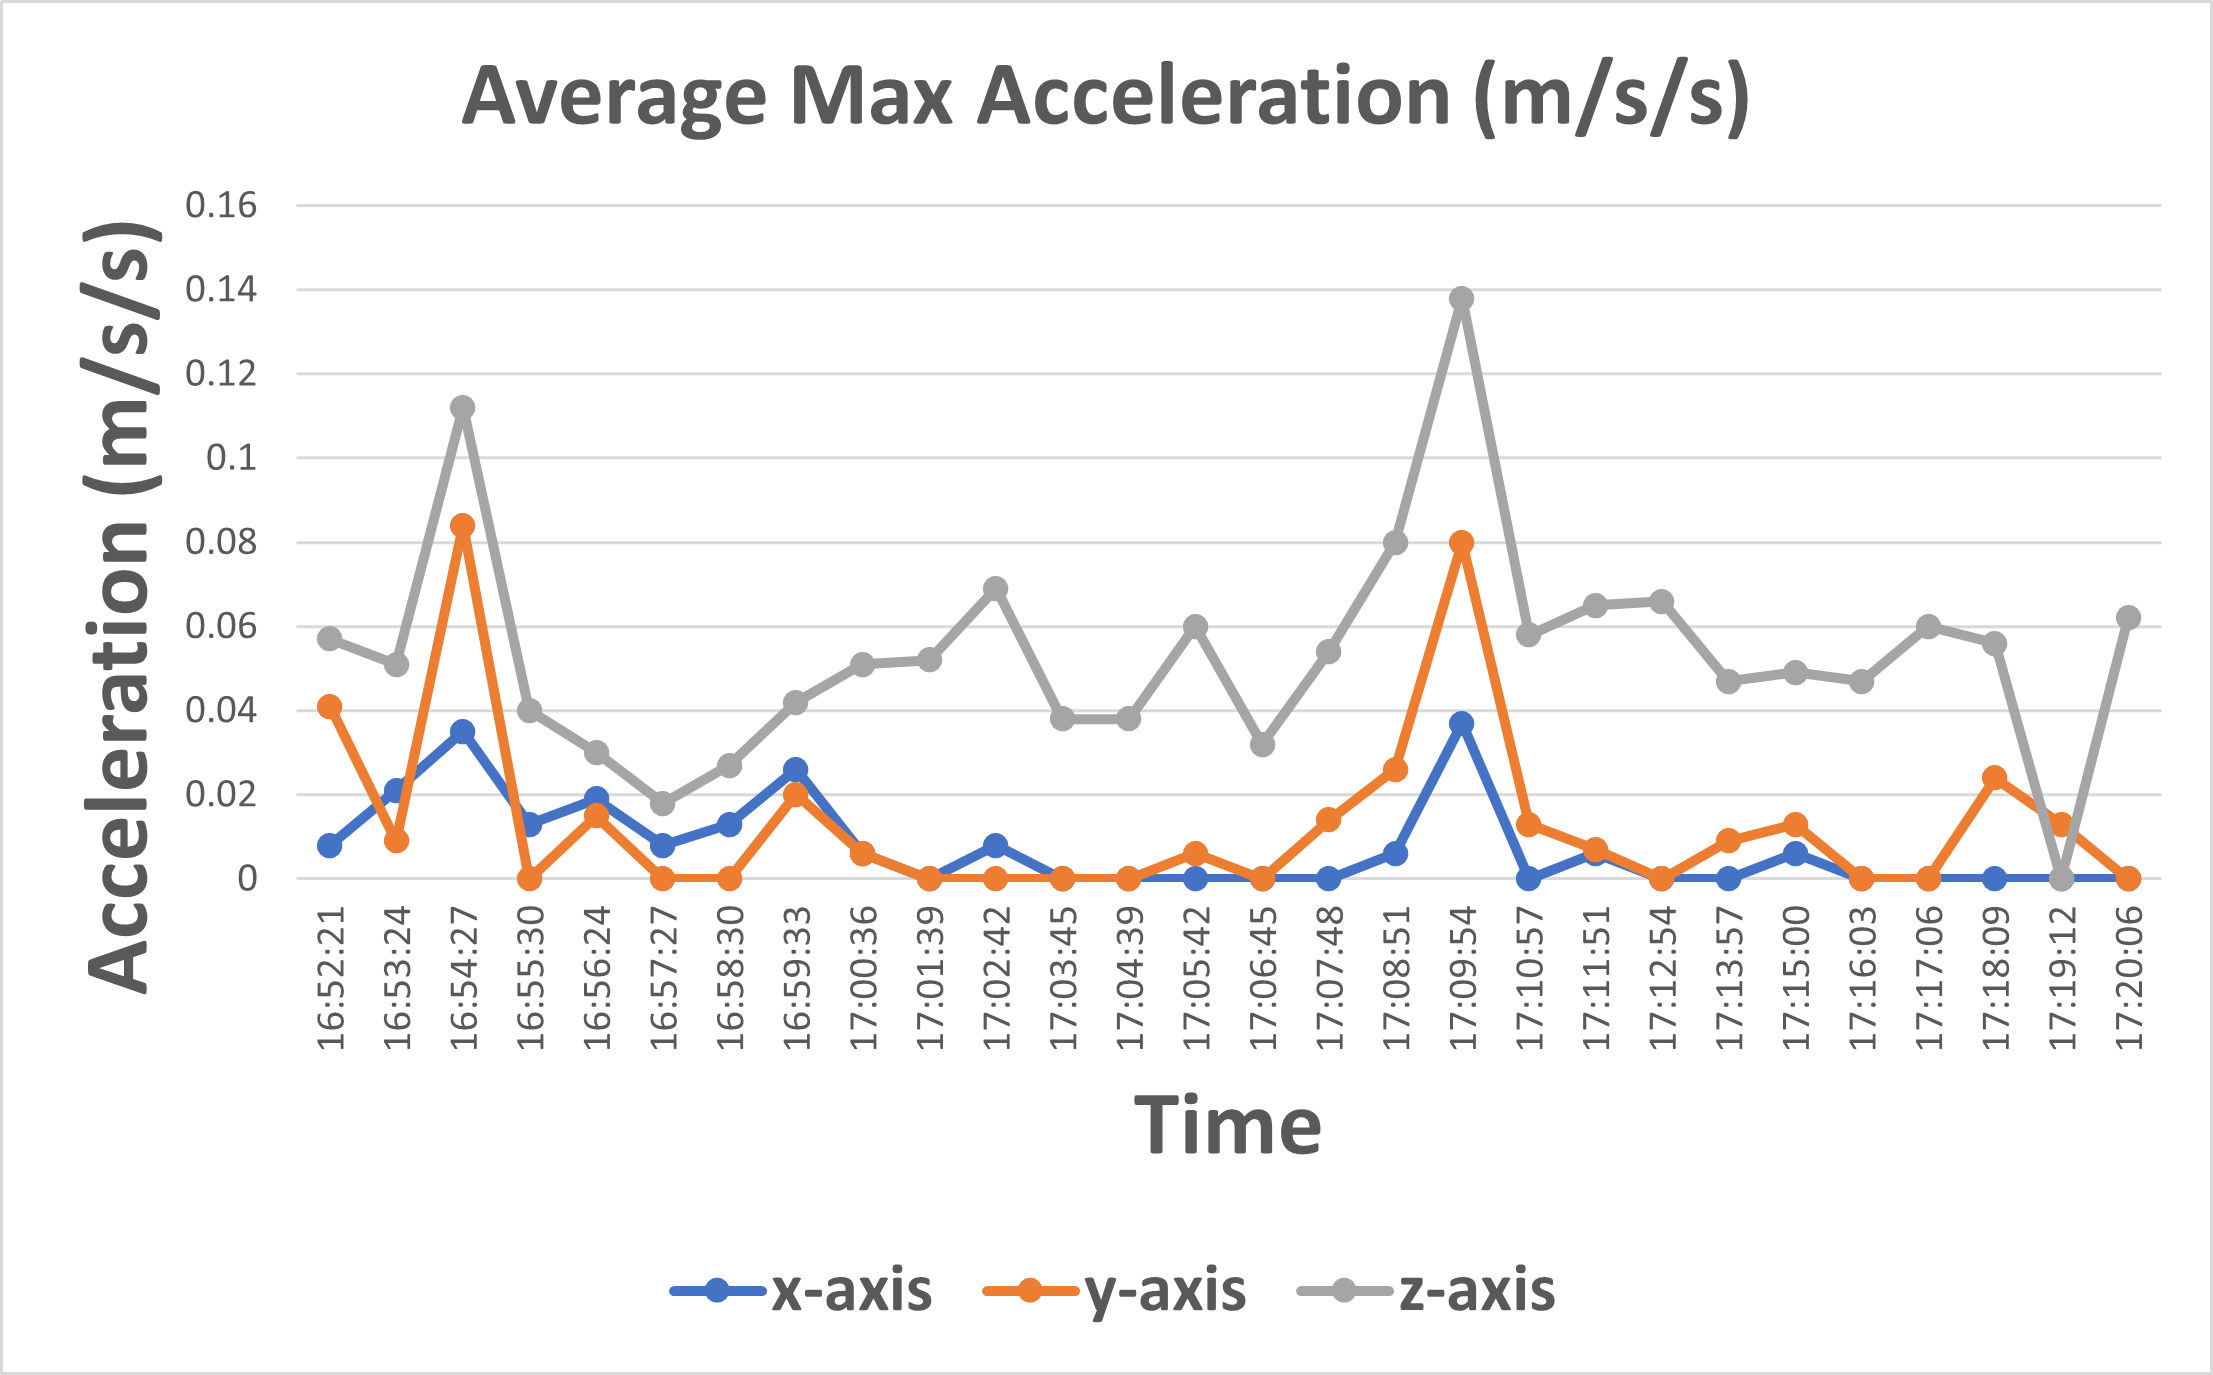
\includegraphics[width=\textwidth]{Sections/Prototype-Testing/proto2-test2-a.png}
	\label{proto2-test2-a}
\end{figure}

\begin{figure}[H]
	\centering
	\caption{Prototype 2: Test 2 Maximum Average Frequency}
	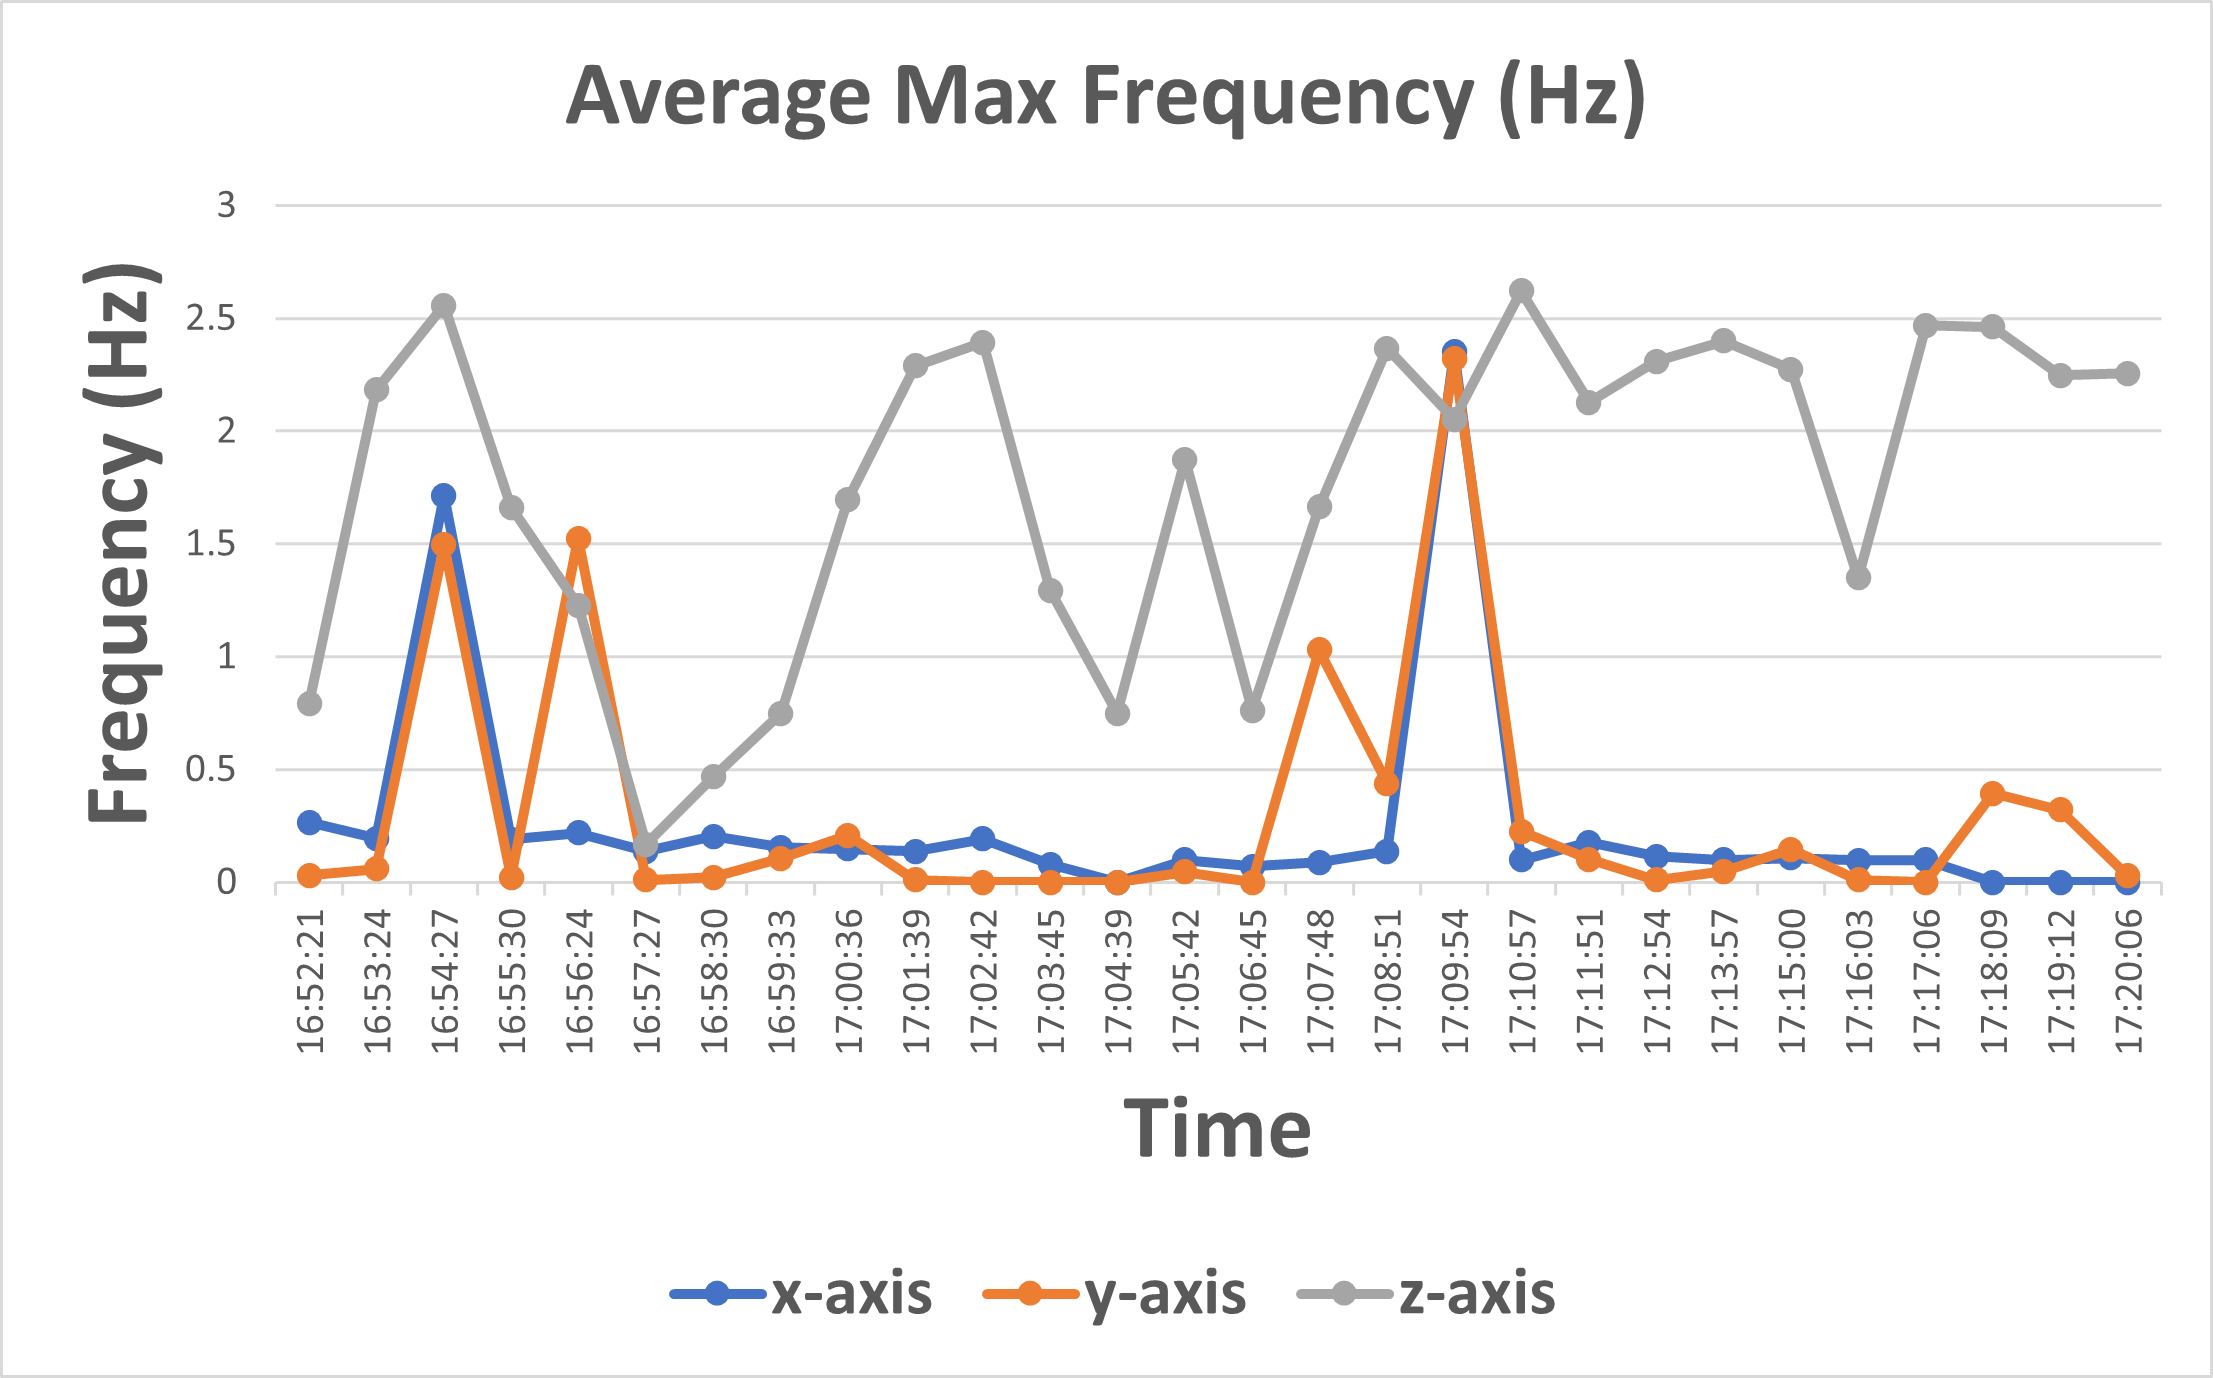
\includegraphics[width=\textwidth]{Sections/Prototype-Testing/proto2-test2-f.png}
	\label{proto2-test2-f}
\end{figure}

\begin{figure}[H]
	\centering
	\caption{Prototype 2: Test 2 SNR}
	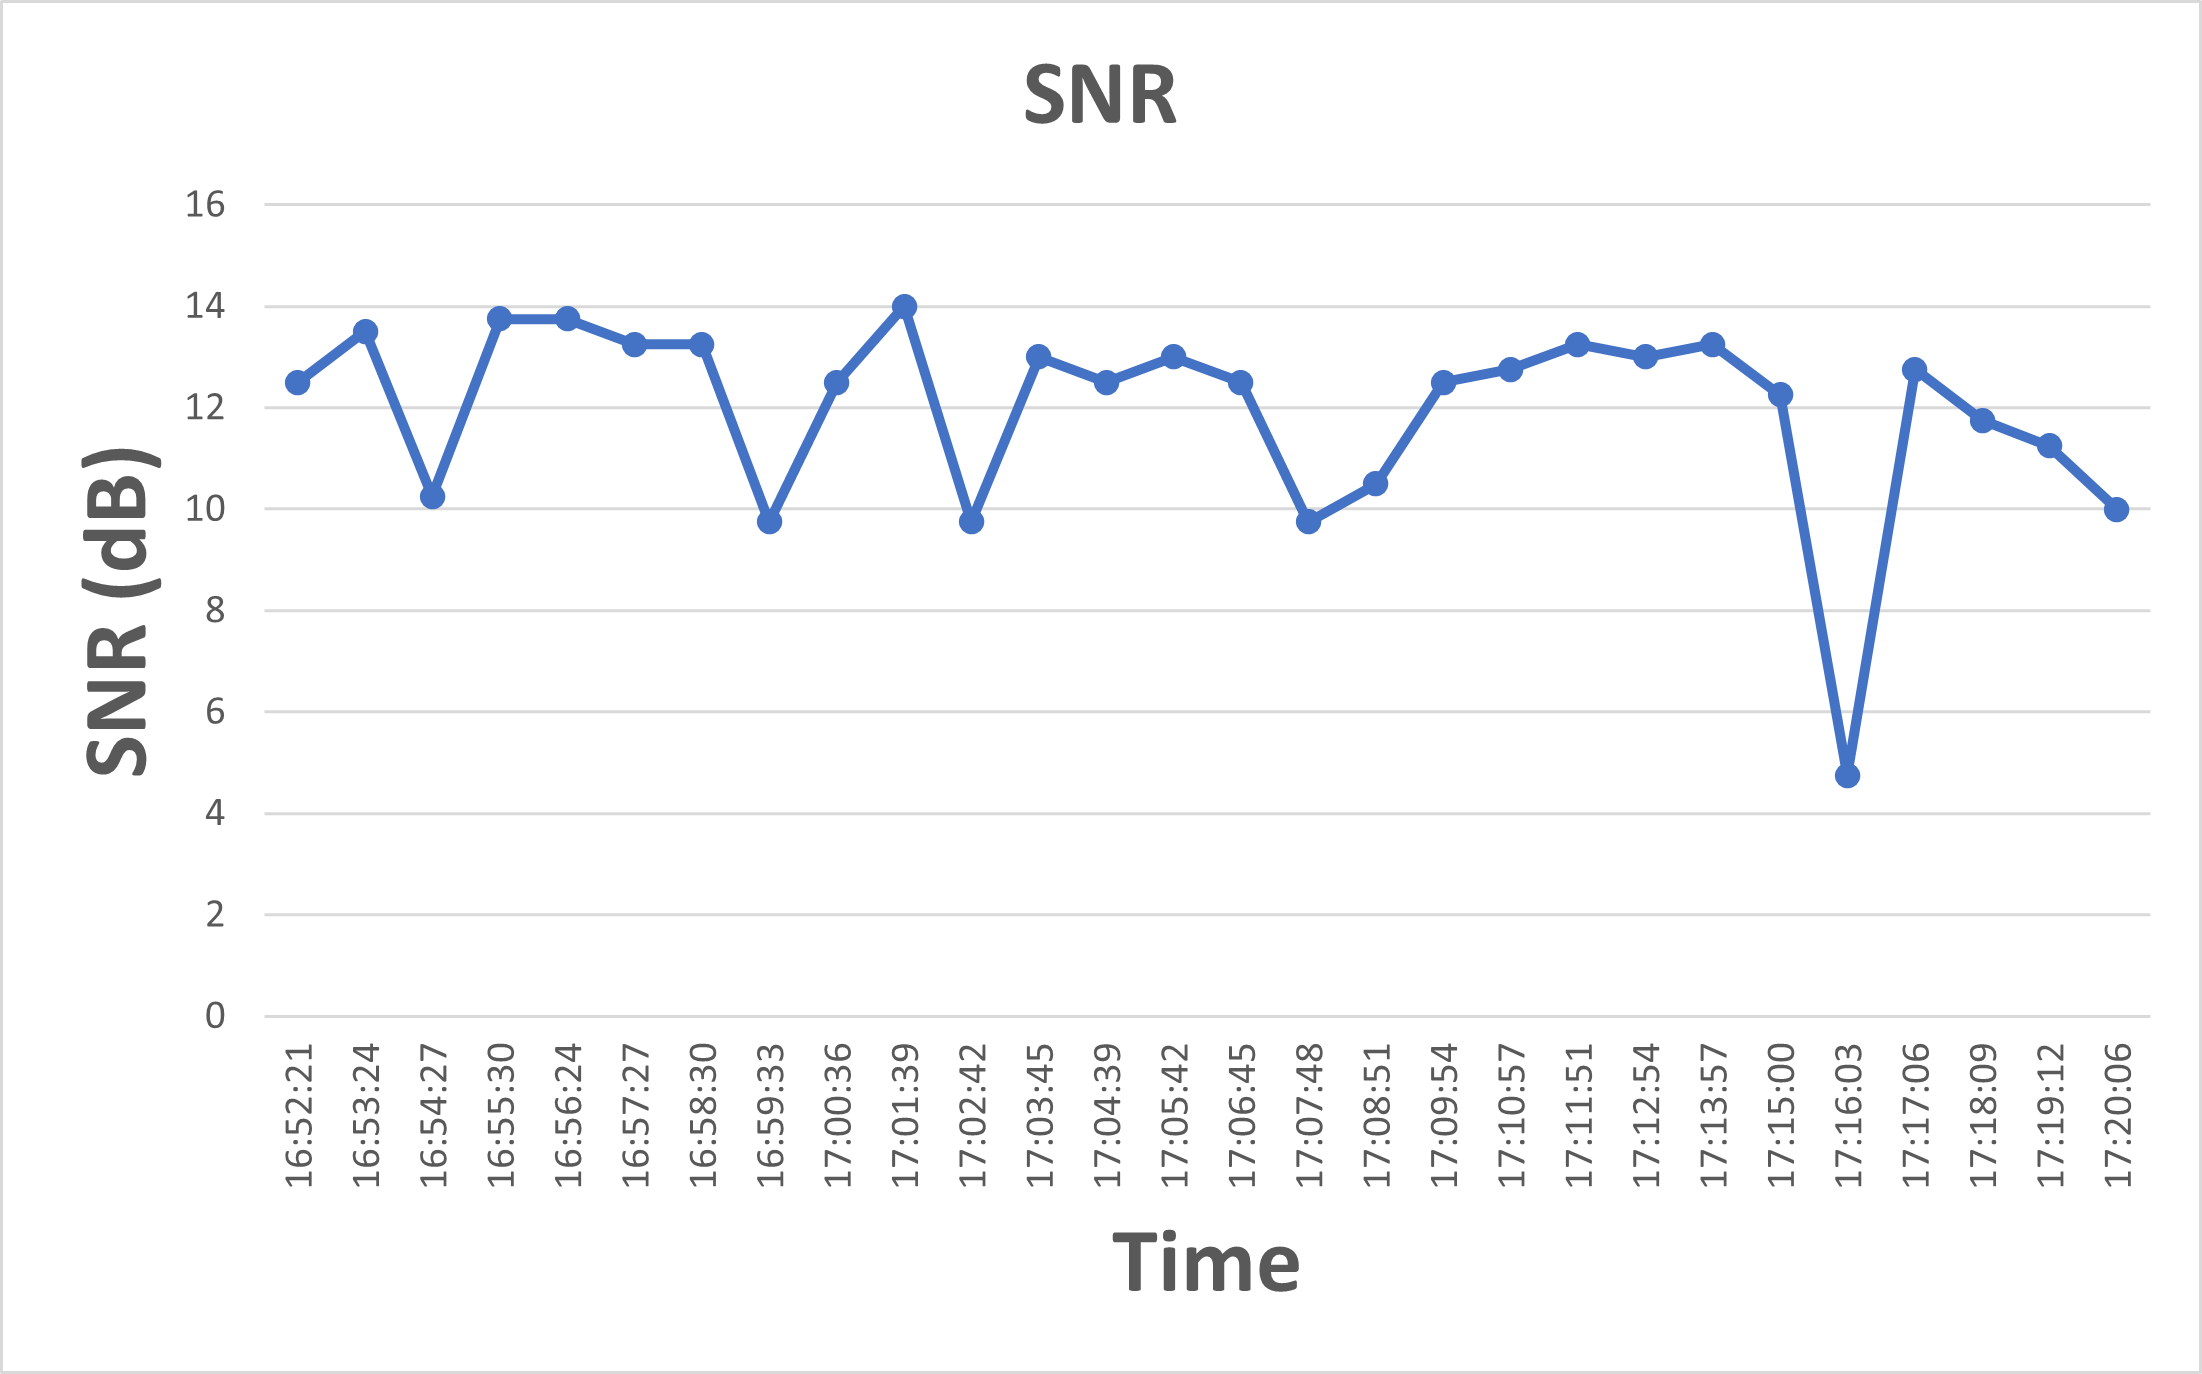
\includegraphics[width=\textwidth]{Sections/Prototype-Testing/proto2-test2-snr.png}
	\label{proto2-test2-snr}
\end{figure}

\begin{figure}[H]
	\centering
	\caption{Prototype 2: Test 2 RSSI}
	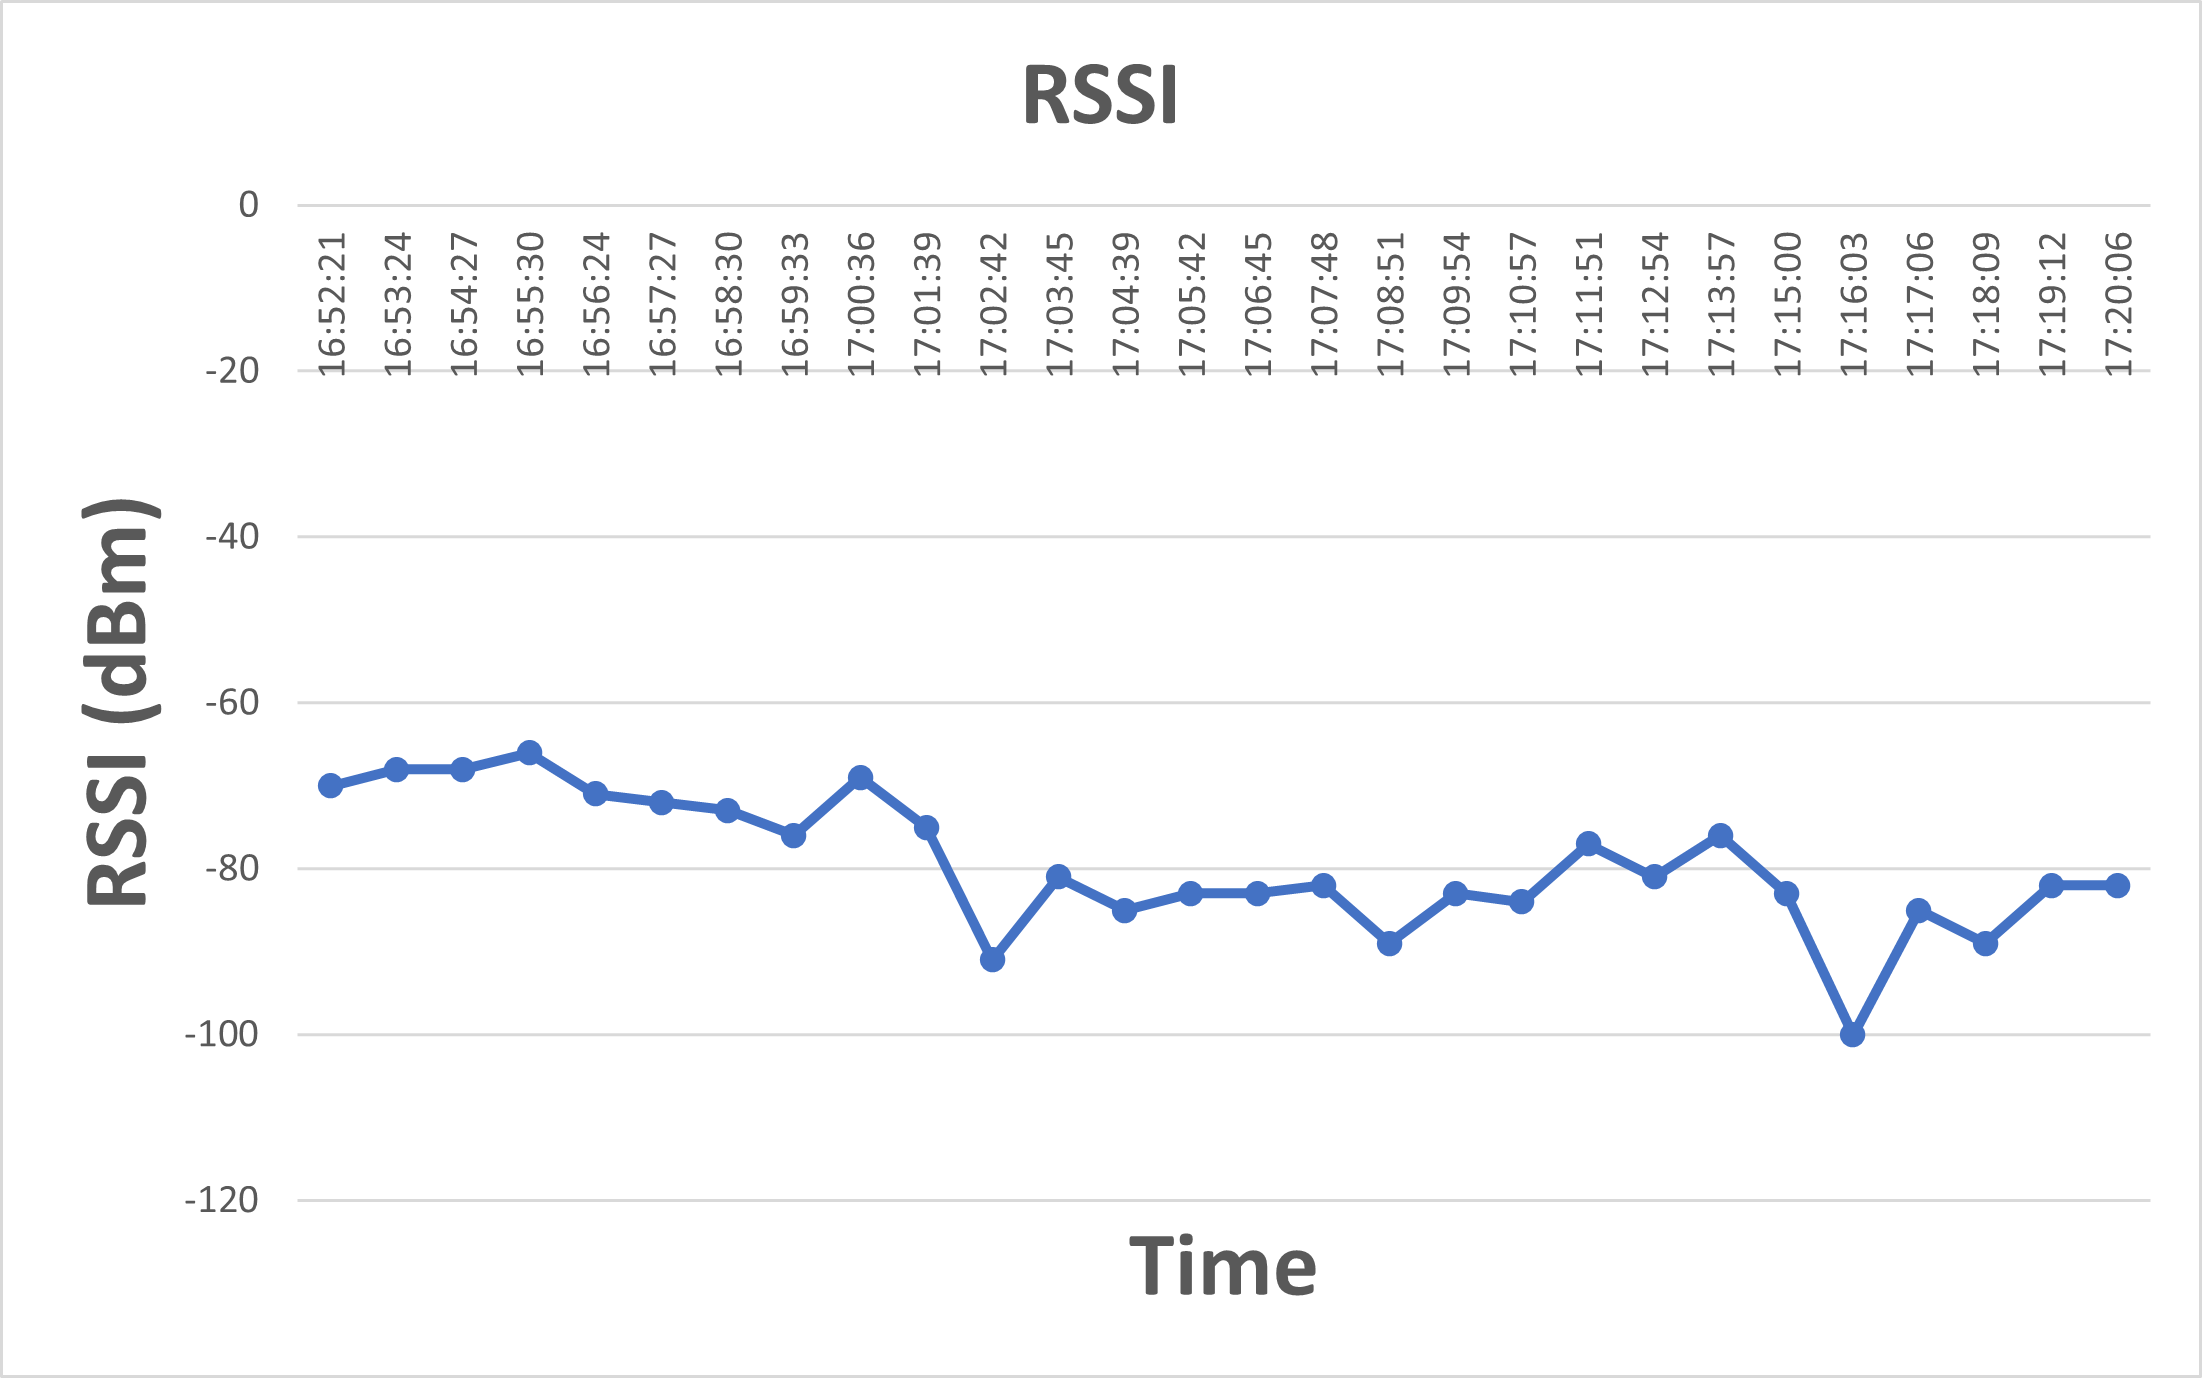
\includegraphics[width=\textwidth]{Sections/Prototype-Testing/proto2-test2-rssi.png}
	\label{proto2-test2-rssi}
\end{figure}

\subsubsection{Prototype 2: Test 3}
Test three was also conducted over a thirty minute period and the enclosure was reinstalled onto the bridge handrail. In this test the noise thresholds were changed to 0.03 for each axis. Packets were transmitted every sixty seconds and each participant fulfilled the same roles specified in test one and two. 
\begin{comment}
\section{Test Results}
\subsection{Prototype 1: Beam Test Reults}
\subsection{Prototype 2: Bridge Test Results}
\end{comment}




\subsubsection{Prototype 2: Test 3 Results}
Test three was conducted with decreased noise thresholds of 0.03 for each axis. Compared to test one, there was a significantly improved response in the x-axis with an average maximum frequency value of 2.5 Hz. This value is also more stable compared to the previous tests with peak frequencies lying between 2 Hz and 3.5 Hz whilst showing the response characteristics of increased vibration from pedestrian load due to the resonance phenomenon. With the insight from all three experiments, it is clear that a noise threshold value of 0.03 for the x-axis was much more representative of the expected 2.2 Hz for the first mode flexural frequency of the bridge. It is also apparent that 0.03 is too low for the other axis as there are elements of cross talk and noise in the y-axis and z-axis frequency response. The noise thresholds for these axis need to be increased to become more representative of the bridge's y-axis and z-axis frequency components.\\\\
In terms of SNR and RSSI, similar values from test one and two were achieved. There was a a -5 dB drop in SNR and -120 dBm drop in RSSI during this test which was the lowest signal drop in all three experiments. It is clear that the direction of the antenna plays a role in the signal strength as tests one and two involve the antenna facing upwards. Regardless of the drop, the resilient nature of LoRaWAN means that the packet was not completely dropped and the signal was able to resume normal functionality. Notably, this drop occurred at 17:43:40 which corresponds to a strong peak in the average max acceleration. This peak may therefore be attributed to noise or corruption and may not be indicative of the bridge's actual acceleration response. 

\begin{figure}[H]
	\centering
	\caption{Prototype 2: Test 3 Maximum Average Acceleration}
	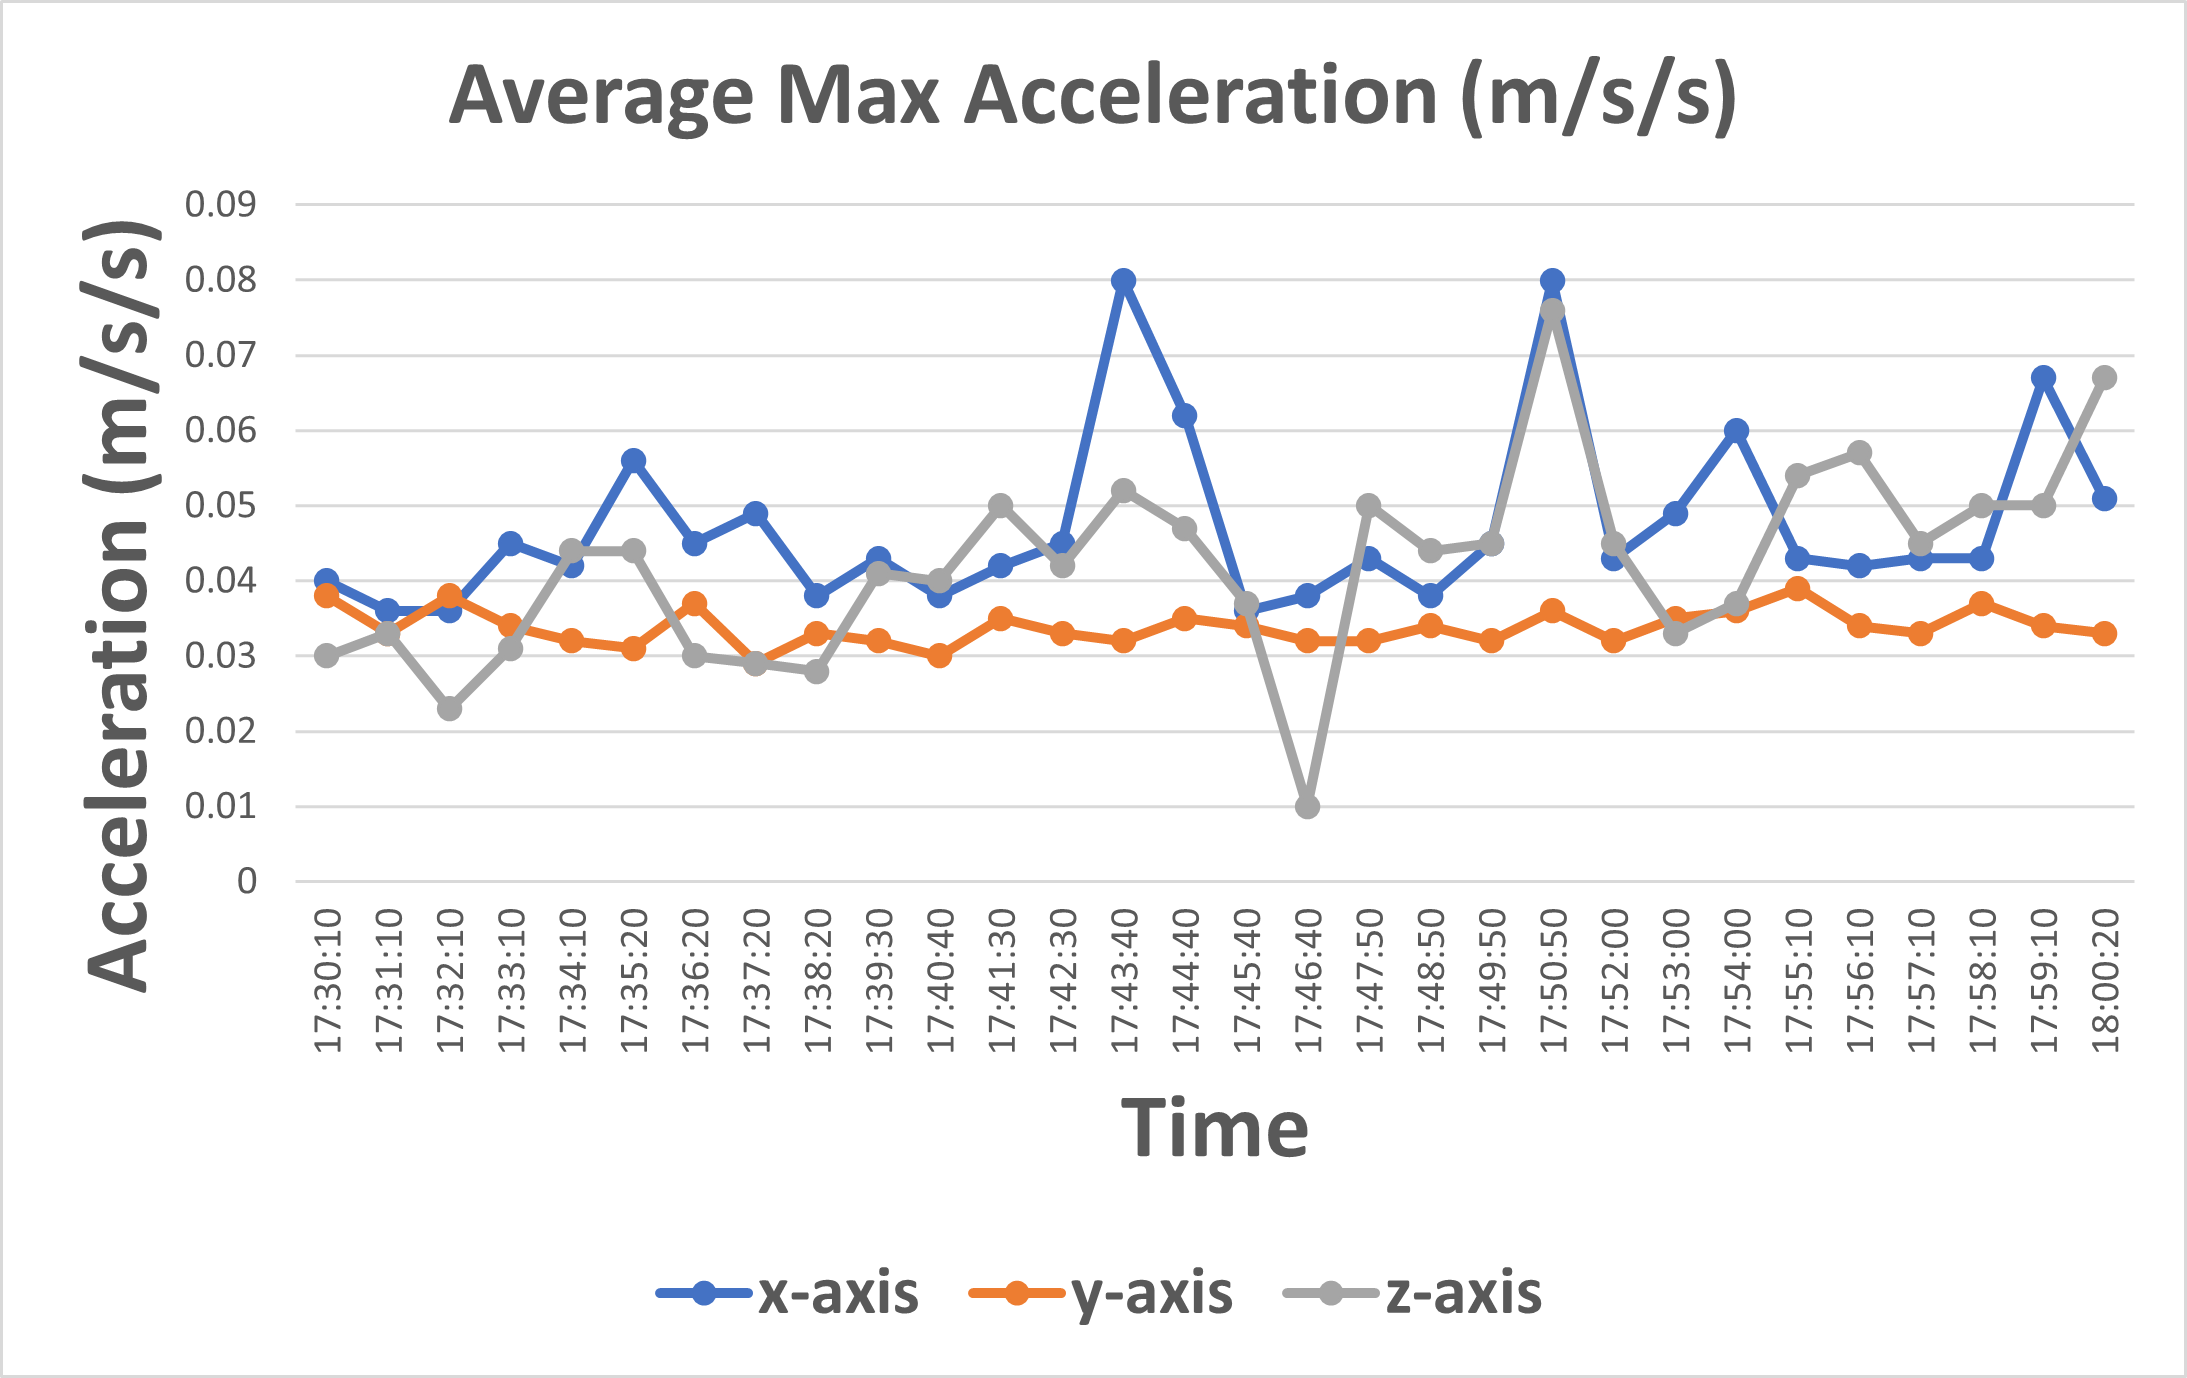
\includegraphics[width=\textwidth]{Sections/Prototype-Testing/proto2-test3-a.png}
	\label{proto2-test3-a}
\end{figure}

\begin{figure}[H]
	\centering
	\caption{Prototype 2: Test 3 Maximum Average Frequency}
	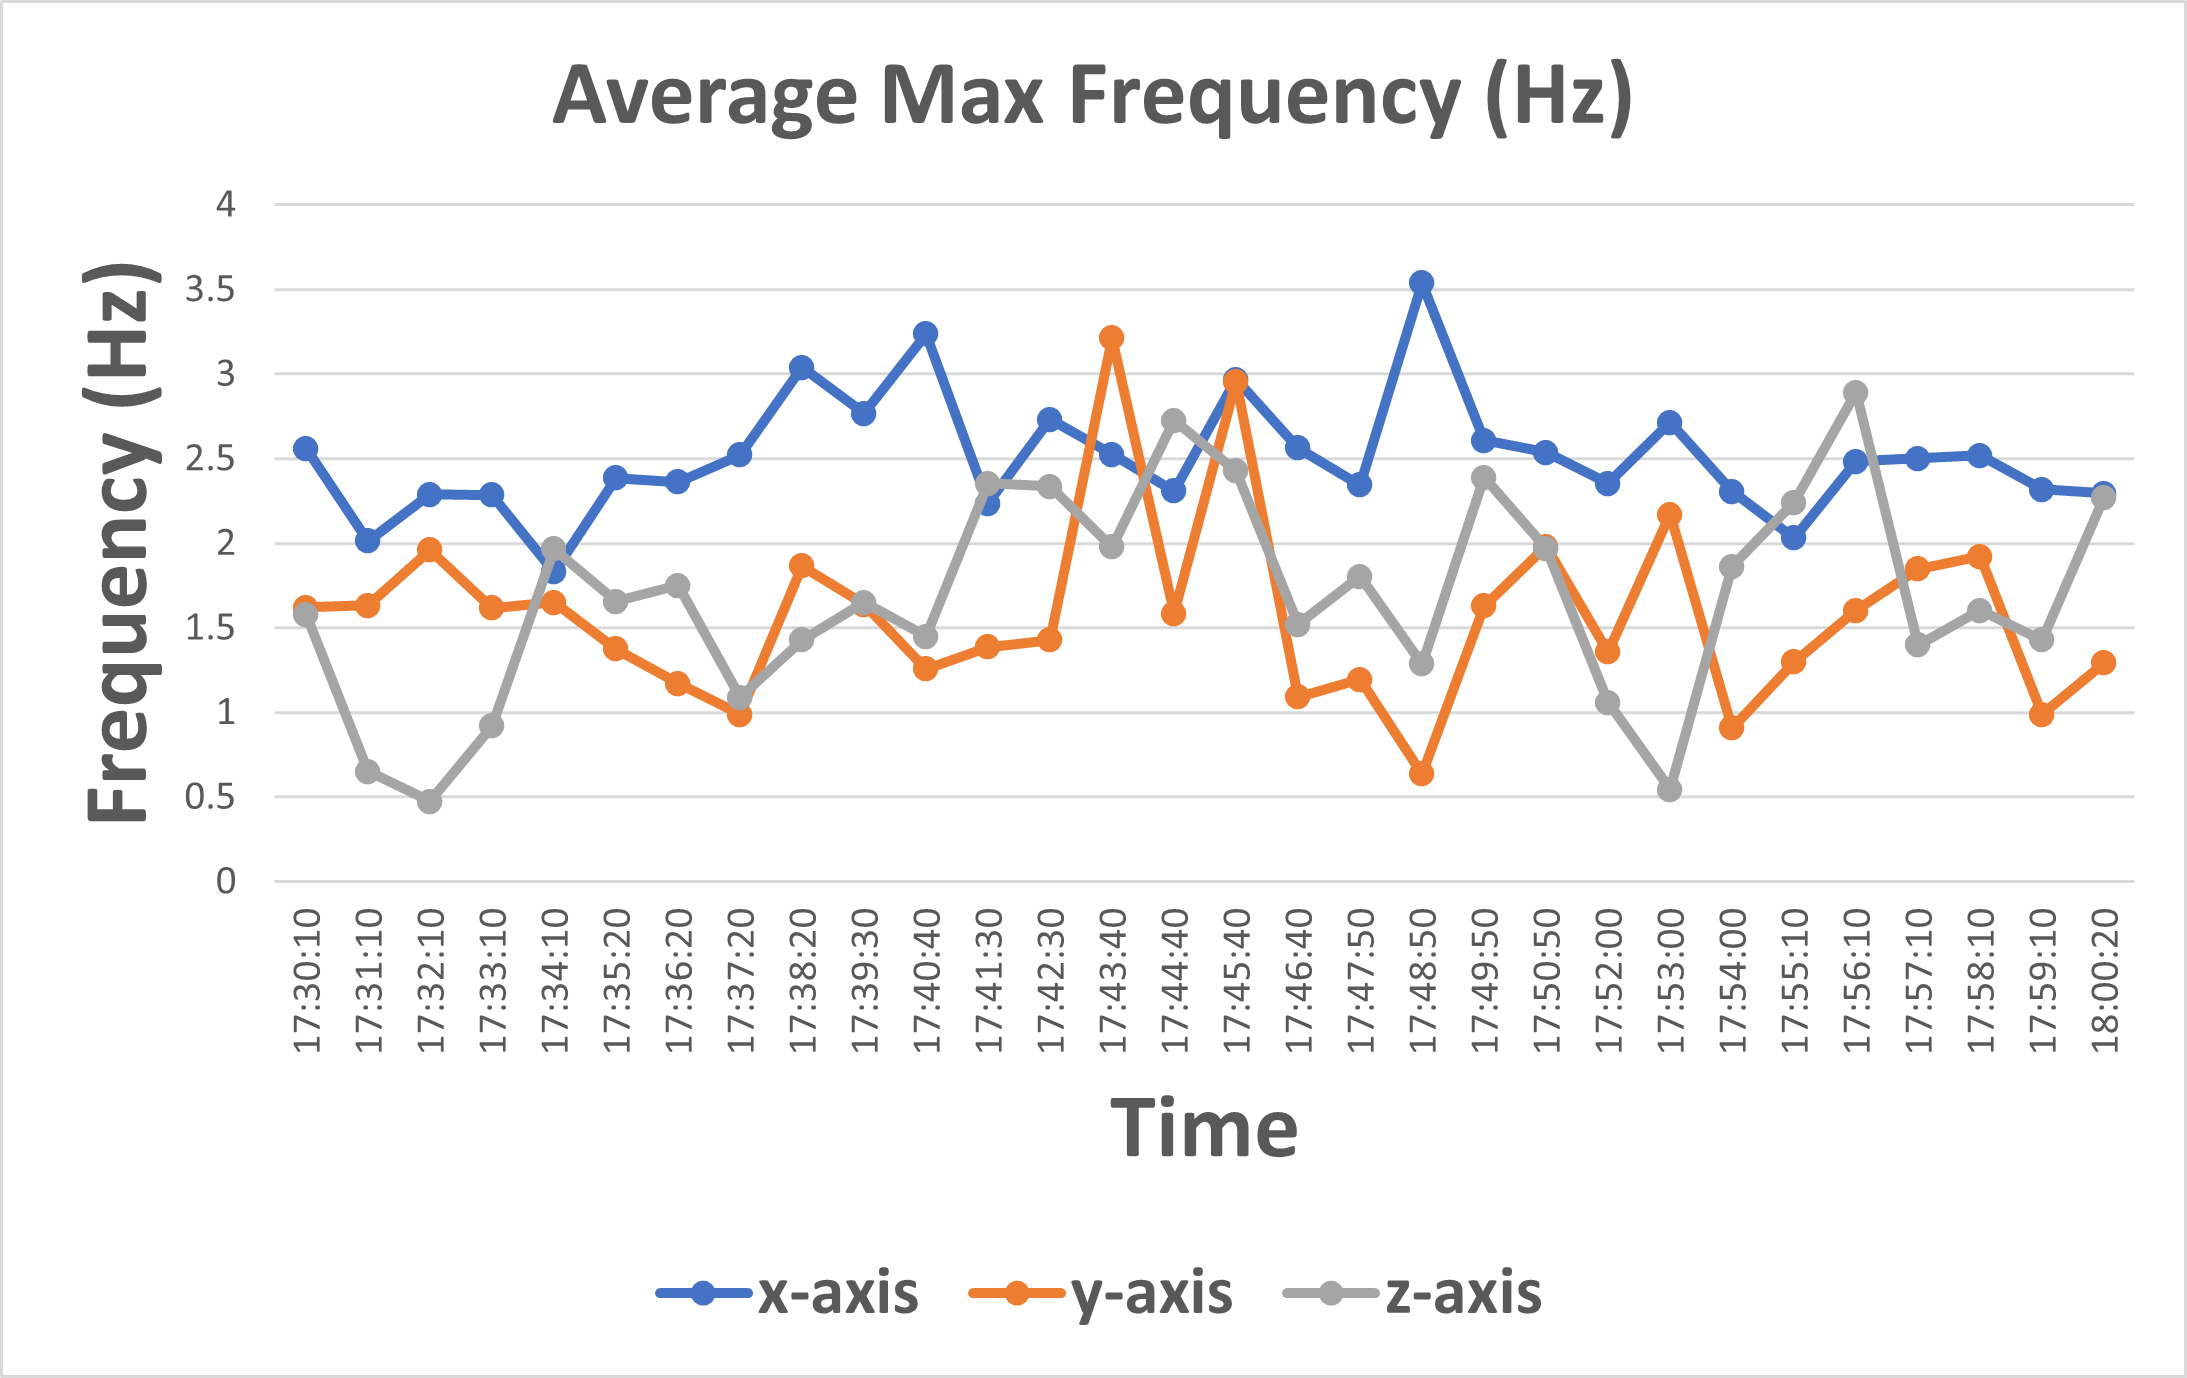
\includegraphics[width=\textwidth]{Sections/Prototype-Testing/proto2-test3-f.png}
	\label{proto2-test3-f}
\end{figure}

\begin{figure}[H]
	\centering
	\caption{Prototype 2: Test 3 SNR}
	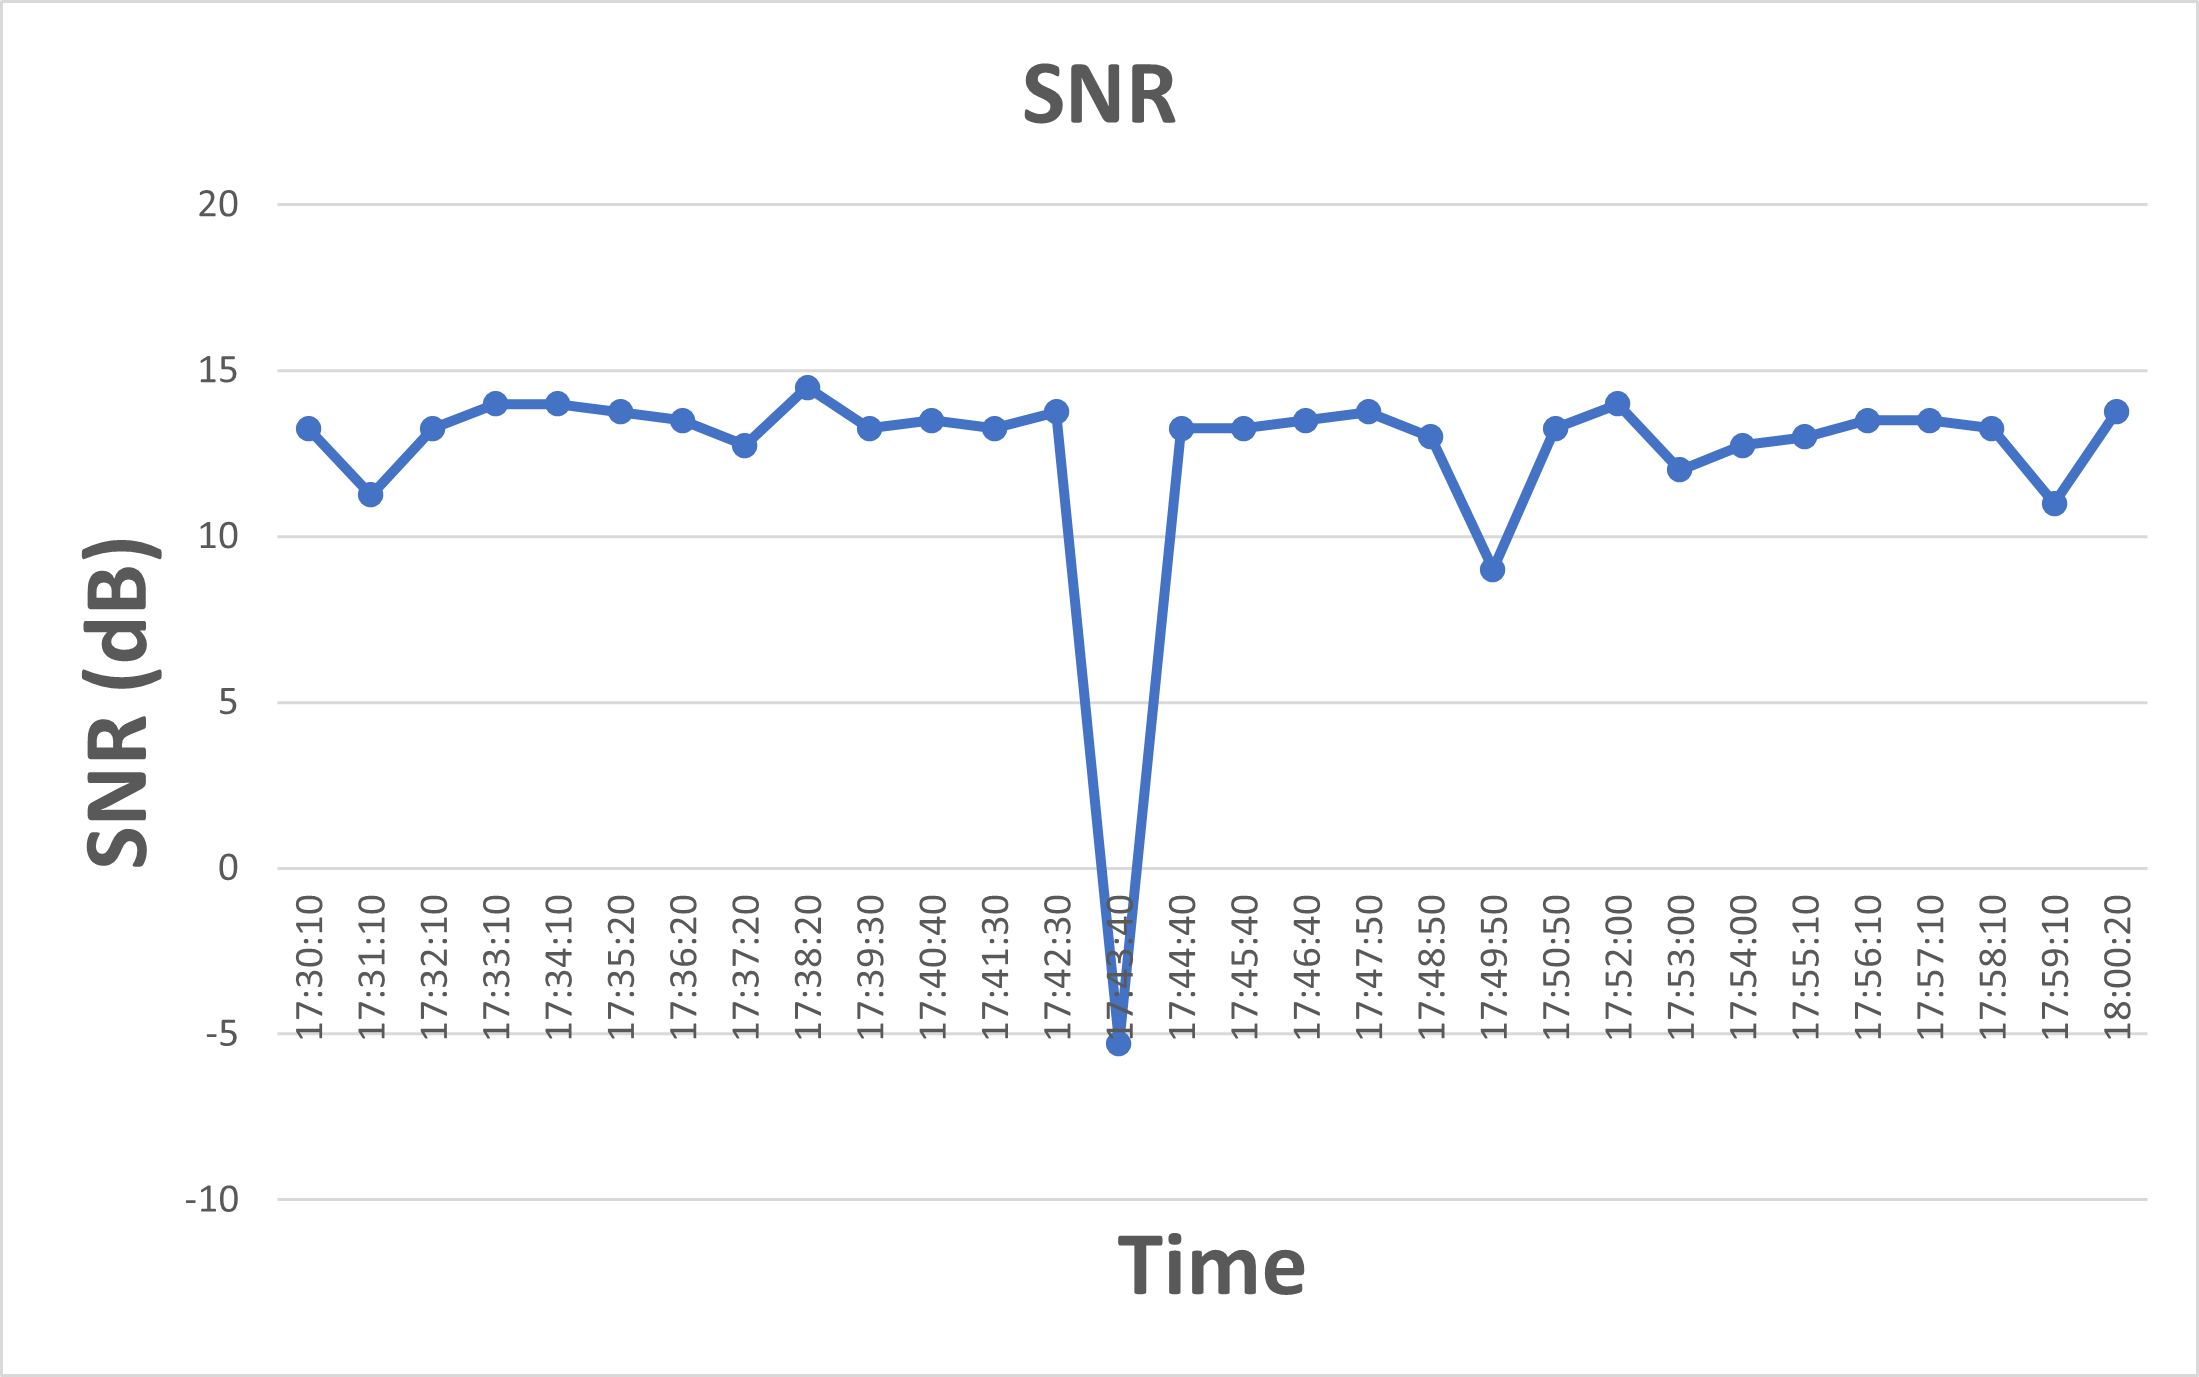
\includegraphics[width=\textwidth]{Sections/Prototype-Testing/proto2-test3-snr.png}
	\label{proto2-test3-snr}
\end{figure}

\begin{figure}[H]
	\centering
	\caption{Prototype 2: Test 3 RSSI}
	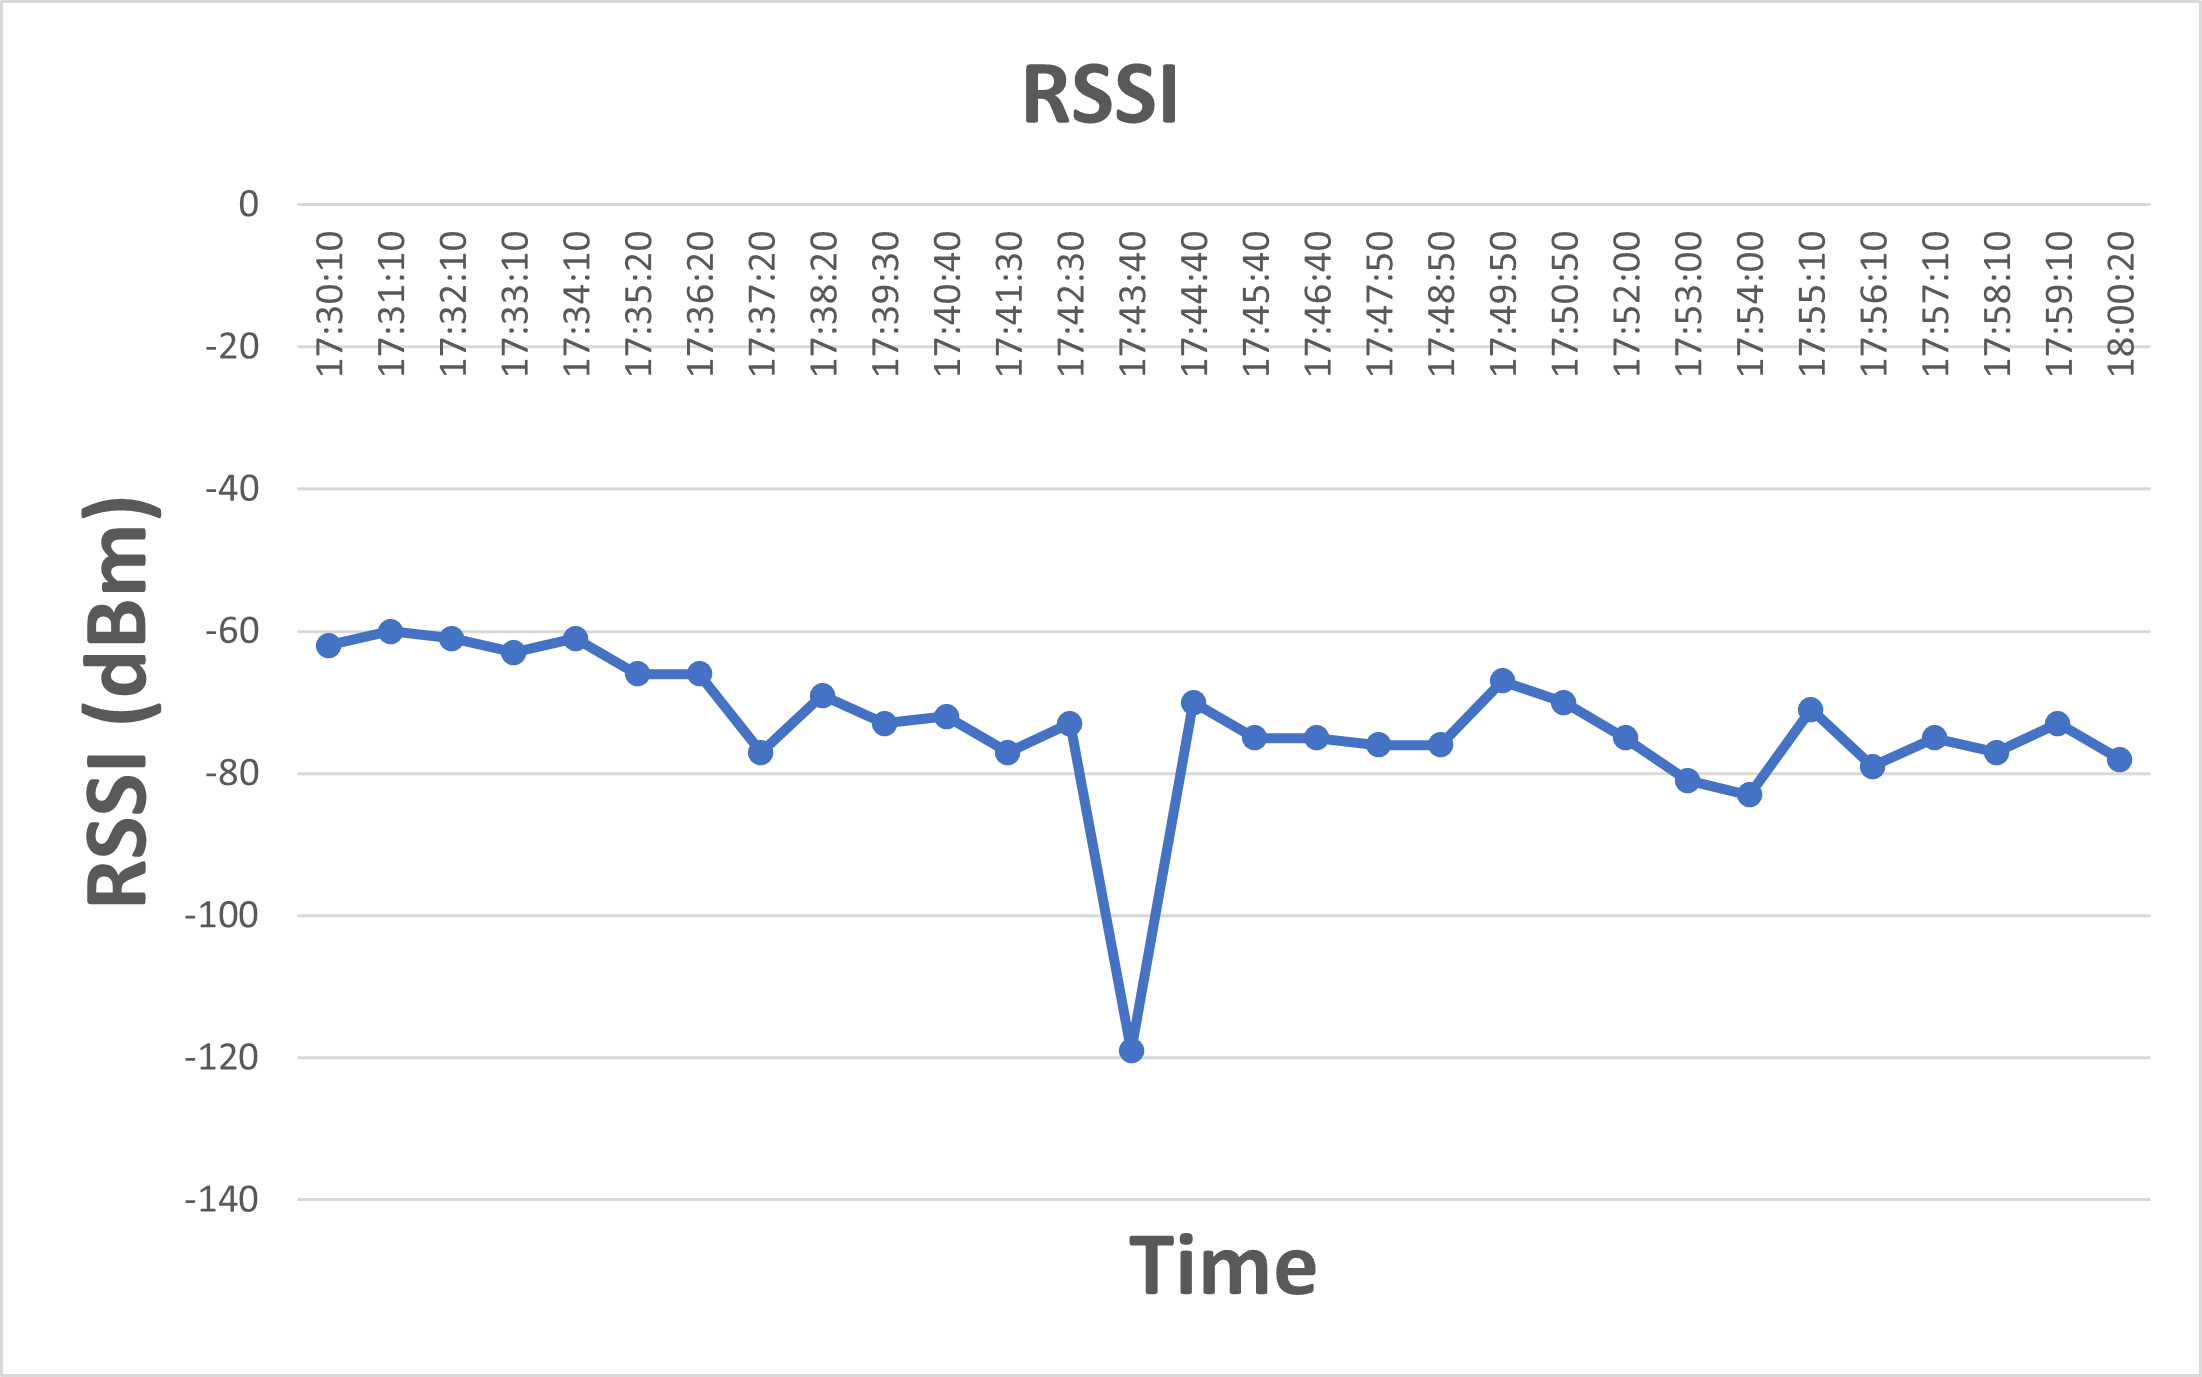
\includegraphics[width=\textwidth]{Sections/Prototype-Testing/proto2-test3-rssi.png}
	\label{proto2-test3-rssi}
\end{figure}











\chapter{Discussions}
\section{Effectiveness of LoRa Node}
The beam laboratory and Griffith footbridge testing demonstrated the effectiveness of LoRa nodes in structural health monitoring as per the following points:
\subsection{FFT Accuracy and Device Calibration} 
The laboratory beam testing confirmed the effectiveness of the FFT computation within the software and the ability to accurately identify peak maximum frequencies. This accuracy was verified with comparison to the first mode fundamental frequency achieved in the Strand7 FE simulation as both achieved peak frequency of 2.4 Hz. Additionally, the device's functionality remained consistent when powered by a battery pack and operating under a lower reference voltage. This illustrates the device's adaptability to different power sources and confirms the successful calibration of the accelerometer which is essential for real-world application and deployment.
\subsection{Low Power}
A multimeter was used to measure the current draw of the device during the FFT computation and LoRa packet transmission when using the battery pack. With 3.0 V input voltage from the two triple A batteries, the current draw of the device was approximately 23.8 mA. The batteries were listed at 1250 mAh which means that prototype two was capable of supporting 52.5 hours of deployment with constant computation load. This is a long lifetime for a prototype, highlighting the low-power nature of LoRa nodes, which can be improved through various metrics which are discussed in the recommendations section. 
\subsection{Noise Thresholds and Response}
Adjustments to the noise thresholds in the acceleration processing greatly influenced the frequency response of the system. Tailoring these values allowed the system to align closely with the first mode fundamental frequency from the FE simulation in the prototype one laboratory beam test, and within 12.8\% of the first mode flexural frequency in the prototype two bridge test. Further trial and error testing can result in a much higher accuracy by further fine tuning the noise threshold parameters. 
\subsection{Impact of Pedestrian Load}
The sensitivity of prototype two to variations in pedestrian load indicate its capability to monitor and interpret external influences on the structure. This responsiveness can further the system's ability to analyse structural behaviour under varying conditions. The impact to the structural health of the bridge can be observed by logging the first mode flexural frequency over long periods of time in a future deployment. This can give indication as to how significant the impact of high pedestrian load or an accident has on the bridge's structural integrity. 

\section{LoRaWAN Signal Strength}
The main limitations of this project exist in the communication range and signal strength of the prototype two deployment. Some characteristics of the LoRaWAN signal strength do show promising prospects for future design revisions which are discussed in the following points:

\subsection{Communication Range}
Prototype one test three confirmed a successful communication range of 200m, showcasing the system's potential for large-scale structural monitoring. However, there were issues involved in the test setup for prototype two. Initially the base station was deployed in a nearby building but was completely closed off to the outside by thick windows. After three to four successful packets, the connection was dropped. This indicates that the prototype two deployment was highly susceptible to obstacles and environmental factors.\\\\
This susceptibility is a result of the antenna, gateway and the environment. The antenna is rated at a gain of -1 dBi in the frequency band of 824 MHz - 960 MHz which restricts the directionality and range of the signal. The gateway was designed for indoor use and so it is likely that the gateway antenna was not designed to penetrate many obstacles such as the thick wall and windows of the enclosed building of the initial base-station deployment. When conducting the range test for prototype one, the door of the laboratory was left open so the test was not isolated from the outside environment. A combination of these factors resulted in a poor communication range for the prototype two implementation, but the exact maximum range for the node to gateway communication in a non-isolated environment is yet to be determined. A antenna with higher gain for the node device and the use of an outdoor gateway would be imperative to achieving a much higher communication range that is more characteristic of LoRaWAN specifications. 
\subsection{Antenna Orientation and Placement}
The results from the prototype two testing indicate that the physical placement and orientation of the antenna on the node device influenced the signal strength and frequency response. Improved SNR and RSSI values were noted when the device was flat and the antenna was directed towards the base station. The enclosure was not specifically designed with this directionality in mind which is an aspect to consider for future revisions.
\subsection{Data Corruption and Signal Resilience}
Even in periods of reduced signal strength, the prototype system was capable of resuming normal functionality which highlights the robustness of LoRaWAN technology. Even with these periods of reduced signal strength, there was no packet loss due to the resilience of the protocol and its ability to transmit with RSSI values as low as -120 dBm \ref{LoRa-SNR-RSSI}. The presence of a strong peak in average max acceleration coinciding with a significant signal drop in test three suggests potential data corruption or noise interference which warrants further investigation. 

\section{Recommendations}
Moving towards future prototypes, revisions and deployments, there are a multitude of recommendations and strategies discovered over the course of this project that are outlined below. 

\subsection{Hardware Selection}
A major limitation faced during the design process was the limited of on board memory for the MKRWAN1300. This is entirely dependent on the intended application of the device but features such as displacement measuring had to be cancelled due to the restricted memory. Besides this, the large amount of GPIO pins on the device and availability of Arduino packages do make the device a great choice as a LoRa node.\\\\
It is recommended that a suitable battery system is chosen for future node implementations. Solar powered batteries offer a great way to increase the battery-life of LoRa nodes. Improvements to the software can be made such as smart-sleeping so that the device is not continuously running computations and draining battery. Implementing a system where the default state of the device is sleep, and then waking up after a certain period of time to sample, compute and transmit would vastly increase battery-life. Improving upon these two aspects of battery and software will vastly increase the time between required maintenance for the LoRa nodes.\\\\
The major difficulty in the hardware selection came down to choosing a suitable gateway. Two gateways were provided by the university, one Arduino branded and the other Dragino. After attempting to use each of these gateways in the LoRaWAN system, it was discovered that neither of them were capable of connecting to TNN in Australia. The Arduino gateway was restricted to European frequencies and the Dragino gateway was not capable of LoRaWAN communication even though it was branded as a LoRa capable device. Therefore, the gateway must be carefully selected with respect to the region of deployment and interactivity with TNN or other network integrations. There is an Arduino branded version of the WisGate Edge Lite 2 which offers the same hardware as the gateway used in this project but with added Arduino firmware for easier integration with the Arduino IoT Cloud. This simplifies the setup of the gateway and devices, but it is advised that future deployments avoid using Arduino in general due to the restrictive nature of the network infrastructure. 

\subsection{Network Infrastructure}
The Arduino IoT Cloud offered an easy to use interface for managing IoT things, cloud variables, dashboards and the TNN back-end integration. However, there are numerous bugs that were found during the implementation. The first bug was the use of an incorrect masking string in the things properties header file that is automatically generated. This is a bug because the TNN integration only works in Australia using the AU915 frequency sub band two which is specified when adding the device to the Arduino IoT cloud. The correct mask is `ff000001f000ffff00020000`.\\\\
Another bug found in the Arduno IoT cloud was the inability to download cloud variable history from the dashboard. Since the cloud variables offer up to three months of data retention with the maker subscription, the cloud variable history at any date can be selected and downloaded to a CSV file. However the cloud variables used in this project were unable to be selected. After contacting Arduino they were able to isolate the bug and implement a fix, but not before the data points for the bridge testing were added to a spreadsheet manually.\\\\
Besides the bugs, Arduino does have good support channels and are able to resolve issues with a fast turn around time. This is not the case for TNN. TNN is a community based platform that is run by volunteers and is not particularly beginner friendly. This makes it hard to fix issues, ask for help and stress test LoRa transmission. Therefore it is the recommendation that future research is conducted to find a suitable replacement. Services such as LoRa Server offer open-source components for building LoRaWAN networks and offers features such as adding integrations with different cloud providers. Amazon Web Services (AWS) and Message Queuing Telemetry Transport (MQTT) can be deployed to handle network messaging which offers the possibility of adding custom storage such as a Structured Query Language (SQL) database. This gives more control over the implementation of the LoRaWAN system, and allows for more research into LoRaWAN communication without the same data policy restrictions enforced by TNN and Arduino IoT Cloud. Additionally, deploying this applications onto a local server eliminate the monthly subscription required for Arduino IoT Cloud and offers as much data retention as needed. 

\subsection{Data Analysis and Monitoring}
In addition to acceleration and frequency response, the incorporation of observational analysis to the system would provide a better understanding of the structural responses of the bridge to pedestrian load. For example, the use of a camera with computer vision and machine learning classifiers could be used to count the number of pedestrians on the bridge at different time stamps to give better context to the vibrational responses. The insights from such an implementation can be further used to improve the predictive capabilities of the system.\\\\
The Arduino IoT Cloud dashboard was helpful in monitoring the testing results in real-time, but a more sophisticated network deployment as previously mentioned offers the capability of post-processing and adding a real-time alert system. Post-processing can be combined with observational analysis to remove noise characteristics evident in the frequency response, and the ability to add maximum threshold values in which non-outlier frequency peaks trigger an alert to the Griffith maintenance staff.

\subsection{Antenna and Gateway Upgrades}
As mentioned in the discussion, the limitations of communication range were attributed to the node antenna and gateway. RAK offers a WisGate Edge Pro outdoor gateway that offers a much larger connection range and is capable of handling transmission through more obstacles. An upgraded gateway matched with an upgraded node antenna and an improved network infrastructure can be used to truly unleash the long range capabilities of the LoRaWAN technology. This kind of upgraded infrastructure can support a vast number of LoRa devices which can be used to attain a more accurate vibrational profile of the bridge, and better indicators to the structural health. Upgrading the gateway and network infrastructure allows for channel hopping, which is sending data over multiple channels to handle larger data packets whilst adhering to Australian communication laws. An upgraded gateway can be placed in a strategical location on the roof of a building on the campus, which can be used to facilitate LoRaWAN systems not only on the Griffith footbridge but for numerous applications campus-wide. 

\subsection{Enclosure and PCB Design} 
A key area for improving the enclosure design is the thickness of the lid. The antenna used in this project was too weak to consistently transmit packets through the enclosure and hence the lid was removed for testing. The lid can also be redesigned to accommodate for a new antenna such as offering an opening for transmission. The enclosure can also be made shorter, but would require a redesign of the PCB with smaller dimensions. There is plenty of empty space on the PCB so this would be an easy fix to implement. 

Implementing these recommendations and strategies can result in an advanced campus-wide LoRaWAN IoT deployment that is based on the insights of this project. Moving to more capable hardware for LoRa nodes, antennas and gateways, and more capable network infrastructure can result in a highly beneficial system not only capable of drawing accurate predictive analysis of the structural health of the Griffith footbridge, but also laying the foundation for any other data acquisition needs within the University. By continually understanding the requirements for LoRaWAN deployment and data acquisition, a more reliable, scalable and insightful IoT architecture can be implemented. 

\section{Conclusion}
The extensive testing and analysis of LoRa nodes within the structural health monitoring of the Griffith University footbridge has substantiated the significant potential of LoRaWAN technology in structural health monitoring. This is evident through the accuracy of FFT computations, calibration of the accelerometer, substantial battery life of the prototypes, sensitivity of the data to pedestrian load and the adaptability to noise thresholds.\\\\
The laboratory beam testing demonstrated the successful implementation of FFT computations within the software to identify peak frequencies, which were found to be consistent with the fundamental frequency achieved in the Strand7 FE simulation. The battery life estimation also highlighted the potential for long-term, low-power monitoring which is critical for real-world applications.\\\\
In addition, the bridge testing indicated the sensitivity of the device to changes in pedestrian load, implying that prototype two was effective in monitoring the external influences on the bridge structure, providing insights into the structural behaviour under different load conditions.\\\\
However, there were constraints in terms of communication range and signal strength, primarily attributed to the indoor gateway, node antenna and environmental obstructions. The limited gain of the node antenna, combined with the initial confined indoor placement of the gateway resulted in challenges when attempting to maintain connection at even a small range.\\\\
With these findings it is clear that future wok needs to focus on specific improvements such as moving away from Arduino and TNN, and moving to more reliable, feature-rich alternative private deployments. This shift would allow for greater control over network messaging, local server deployment, eliminating subscriptions and offer more extensive data retention, promoting in house testing and future LoRa research.\\\\
The addition of observational analysis of pedestrian load, improvements in battery technology and software, and upgrades to the enclosure design are recommended for future revisions. Upgrading the node antenna and gateway would also be beneficial to extending the communication range and facilitate channel hopping, allowing for larger data packets and more reliable coverage.\\\\
Overall, the work conducted in this project lays the groundwork for future LoRaWAN-based IoT architecture, specifically in the field of structural health monitoring systems. It underscores the potential and versatility of LoRaWAN technology, but also highlights the need for careful consideration in hardware selection, network infrastructure and sophisticated data analysis methods. With the recommended upgrades, improvements and strategies, the existing system can be evolved into a formidable, high-capacity LoRaWAN network. This advanced infrastructure would not only revolutionize the structural health monitoring of the Griffith University footbridge, but could also potentially transform the entire landscape of large-scale, real-time structural health monitoring, serving as the blueprint for future IoT infrastructures in the domain of structural monitoring. 



% IMPORTANT: Latex special characters are: # $ % & \ ^ _ { } ~. To avoid mistakes when compiling try writing \ before. For: \ use \textbackslash ; for ^ \textasciitilde and ~ \textasciicircum.

%     Example of figure:
%     \begin{figure}[H]
%     	\ffigbox[\FBwidth] {
%     	\caption[Name as seen in index]{Figure name}
%     	}
%     	{\includegraphics[scale=0.6]{imagenes/creativecommons.png}}
%     \end{figure}
    

%     Example of table:S
% \begin{table}[H]
% 	\ttabbox[\FBwidth]
% 	{\caption{Lorem ipsum}}
% 	{\begin{tabular}{|c|P{1.5cm}|c|P{1.5cm}|P{2cm}|c|P{1.5cm}|P{2cm}|}
% 		\hline
% 		\multicolumn{2}{|c|}{\textbf{I}} & \multicolumn{2}{c|}{\textbf{II}} & \multicolumn{3}{c|}{\textbf{III}} & \textbf{IV} \\
% 		\hline
% 		x & y & x & y & x & y & x & y \\
% 		\hline
% 		10.0 & 8.04 & 10.0 & 9.14 & 10.0 & 7.46 & 8.0 & 6.58 \\
% 		\hline
% 		8.0 & 6.95 & 8.0 & 8.14 & 8.0 & 6.77 & 8.0 & 5.76 \\
% 		\hline
% 		13.0 & 7.58 & 13.0 & 8.74 & 13.0 & 12.74 & 8.0 & 7.71 \\
% 		\hline
% 		9.0 & 8.81 & 9.0 & 8.77 & 9.0 & 7.11 & 8.0 & 8.84 \\
% 		\hline
% 		11.0 & 8.33 & 11.0 & 9.26 & 11.0 & 7.81 & 8.0 & 8.47 \\
% 		\hline
% 		14.0 & 9.96 & 14.0 & 8.10 & 14.0 & 8.84 & 8.0 & 7.04 \\
% 		\hline
% 		6.0 & 7.24 & 6.0 & 6.13 & 6.0 & 6.08 & 8.0 & 5.25 \\
% 		\hline
% 		4.0 & 4.26 & 4.0 & 3.10 & 4.0 & 5.39 & 19.0 & 12.50 \\
% 		\hline
% 		12.0 & 10.84 & 12.0 & 9.13 & 12.0 & 8.15 & 8.0 & 5.56 \\
% 		\hline
% 		7.0 & 4.82 & 7.0 & 7.26 & 7.0 & 6.42 & 8.0 & 7.91 \\
% 		\hline
% 		5.0 & 5.68 & 5.0 & 4.74 & 5.0 & 5.73 & 8.0 & 6.89 \\
% 		\hlineS
% 		\multicolumn{5}{l}{Source: BOE}
% 	\end{tabular}}
% \end{table}


% Start writing here----------------------------------------------------


%----------
%	Bibliography
%----------	

\clearpage
%\addcontentsline{toc}{chapter}{Bibliography}

%\printbibliography
\bibliography{References}


%----------
%	Appendix
%----------	

% If your work includes Appendix, you can uncomment the following lines
\chapter {Appendix}
\pagenumbering{gobble} % Appendix pages are not numbered
\section{Bill of Materials}
\subsection{Prototype 1 Bill of Materials}
\begin{table}[h]
\begin{tabular}{|cc|c|cc}
\hline
\multicolumn{1}{|c|}{\textbf{Item}}                                                                & \textbf{No.} & \textbf{Total Cost} & \multicolumn{1}{c|}{\textbf{Supplier}} & \multicolumn{1}{c|}{\textbf{Function}}                                                                                                                                                          \\ \hline
\multicolumn{1}{|c|}{\begin{tabular}[c]{@{}c@{}}Arduino\\ MKRWAN1300\end{tabular}}                 & 2            & \$135.04            & \multicolumn{1}{c|}{Arduino}           & \multicolumn{1}{c|}{\begin{tabular}[c]{@{}c@{}}Microcontroller used as\\ LoRaWAN node. \\ Responsible for acceleration\\ and frequency computations, \\ and payload transmission.\end{tabular}} \\ \hline
\multicolumn{1}{|c|}{\begin{tabular}[c]{@{}c@{}}Arduino RF antenna\\ (X000016)\end{tabular}}       & test2        & \$8.74              & \multicolumn{1}{c|}{DigiKey}           & \multicolumn{1}{c|}{\begin{tabular}[c]{@{}c@{}}RF antenna used for LoRa \\ packet transmission.\end{tabular}}                                                                                   \\ \hline
\multicolumn{1}{|c|}{\begin{tabular}[c]{@{}c@{}}Accelerometer\\ (ADXL335)\end{tabular}}            & 1            & \$26.44             & \multicolumn{1}{c|}{DigiKey}           & \multicolumn{1}{c|}{\begin{tabular}[c]{@{}c@{}}Accelerometer used for \\ acceleration sampling.\end{tabular}}                                                                                   \\ \hline
\multicolumn{1}{|c|}{\begin{tabular}[c]{@{}c@{}}Breadboard 400 Tie\\ points (PB8820)\end{tabular}} & 1            & \$8.85              & \multicolumn{1}{c|}{Jaycar}            & \multicolumn{1}{c|}{\begin{tabular}[c]{@{}c@{}}Breadboard used for \\ transmitting node.\end{tabular}}                                                                                          \\ \hline
\multicolumn{1}{|c|}{\begin{tabular}[c]{@{}c@{}}Breadboard 170 \\ points (PB8817)\end{tabular}}    & 1            & \$5.95              & \multicolumn{1}{c|}{Jaycar}            & \multicolumn{1}{c|}{\begin{tabular}[c]{@{}c@{}}Breadboard used for \\ receiving node.\end{tabular}}                                                                                             \\ \hline
\multicolumn{1}{|c|}{AAA battery holder}                                                           & 1            & \$4.50              & \multicolumn{1}{c|}{Jaycar}            & \multicolumn{1}{c|}{\begin{tabular}[c]{@{}c@{}}Battery holder with switch \\ connected to terminal block\\ of the MKRWAN1300.\end{tabular}}                                                     \\ \hline
\multicolumn{1}{|c|}{AAA lithium battery}                                                          & 2            & \$16.95             & \multicolumn{1}{c|}{Jaycar}            & \multicolumn{1}{c|}{\begin{tabular}[c]{@{}c@{}}Powers MKRWAN1300 with\\ total 3.0V.\end{tabular}}                                                                                               \\ \hline
\multicolumn{2}{|c|}{\textbf{Total Cost:}}                                                                        & \textbf{\$206.57}   &                                        &                                                                                                                                                                                                 \\ \cline{1-3}
\end{tabular}
\caption{Prototype 1 Bill of Materials}
\label{proto1-bom}
\end{table}

\subsection{Prototype 2 Bill of Materials}
\begin{table}[H]
\begin{tabular}{|cc|c|cc}
\hline
\multicolumn{1}{|c|}{\textbf{Item}}                                                                                               & \textbf{No.} & \textbf{Total Cost} & \multicolumn{1}{c|}{\textbf{Supplier}}                                               & \multicolumn{1}{c|}{\textbf{Function}}                                                                                       \\ \hline
\multicolumn{1}{|c|}{\begin{tabular}[c]{@{}c@{}}Arduino Maker\\ Subscription\end{tabular}}                                        & 1            & \$10.77             & \multicolumn{1}{c|}{Arduino}                                                         & \multicolumn{1}{c|}{\begin{tabular}[c]{@{}c@{}}Unlimited cloud variables\\ and 3 month data retention.\end{tabular}}         \\ \hline
\multicolumn{1}{|c|}{\begin{tabular}[c]{@{}c@{}}M3 machine screw\\ 20mm\end{tabular}}                                             & 25           & \$4.95              & \multicolumn{1}{c|}{\begin{tabular}[c]{@{}c@{}}Core\\ Electronics\end{tabular}}      & \multicolumn{1}{c|}{\begin{tabular}[c]{@{}c@{}}Used to secure front and \\ back plate of enclosure.\end{tabular}}            \\ \hline
\multicolumn{1}{|c|}{\begin{tabular}[c]{@{}c@{}}M3 machine screw \\ 14mm\end{tabular}}                                            & 25           & \$3.35              & \multicolumn{1}{c|}{\begin{tabular}[c]{@{}c@{}}Core\\ Electronics\end{tabular}}      & \multicolumn{1}{c|}{\begin{tabular}[c]{@{}c@{}}Used to secure lid of \\ enclosure.\end{tabular}}                             \\ \hline
\multicolumn{1}{|c|}{\begin{tabular}[c]{@{}c@{}}Heat-set insert \\ soldering iron tip\end{tabular}}                               & 1            & \$21.88             & \multicolumn{1}{c|}{\begin{tabular}[c]{@{}c@{}}Core \\ Electronics\end{tabular}}     & \multicolumn{1}{c|}{\begin{tabular}[c]{@{}c@{}}Used to install heat-set\\ inserts.\end{tabular}}                             \\ \hline
\multicolumn{1}{|c|}{\begin{tabular}[c]{@{}c@{}}M3 brass heat-set\\ inserts 4mm\end{tabular}}                                     & 50           & \$11.95             & \multicolumn{1}{c|}{\begin{tabular}[c]{@{}c@{}}Core \\ Electronics\end{tabular}}     & \multicolumn{1}{c|}{\begin{tabular}[c]{@{}c@{}}Used to secure front and\\ back plate, and lid of \\ enclosure.\end{tabular}} \\ \hline
\multicolumn{1}{|c|}{\begin{tabular}[c]{@{}c@{}}M2 screw and nut \\ mounting kit\end{tabular}}                                    & 1            & \$23.95             & \multicolumn{1}{c|}{\begin{tabular}[c]{@{}c@{}}Core \\ Electrnoics\end{tabular}}     & \multicolumn{1}{c|}{\begin{tabular}[c]{@{}c@{}}Used to mount PCB in \\ enclosure.\end{tabular}}                              \\ \hline
\multicolumn{1}{|c|}{M10 bolt and nut}                                                                                            & 1            & \$2.68              & \multicolumn{1}{c|}{\begin{tabular}[c]{@{}c@{}}Bunnings\\ Warehouse\end{tabular}}    & \multicolumn{1}{c|}{\begin{tabular}[c]{@{}c@{}}Used to secure enclosure\\ to bridge.\end{tabular}}                           \\ \hline
\multicolumn{1}{|c|}{\begin{tabular}[c]{@{}c@{}}Threadlocker \\ Loctite 10ml\end{tabular}}                                        & 1            & \$15.02             & \multicolumn{1}{c|}{\begin{tabular}[c]{@{}c@{}}Bunnings\\ Warehouse\end{tabular}}    & \multicolumn{1}{c|}{Used to secure all screws.}                                                                              \\ \hline
\multicolumn{1}{|c|}{\begin{tabular}[c]{@{}c@{}}M2 machine screw \\ 30mm\end{tabular}}                                            & 20           & \$8.00              & \multicolumn{1}{c|}{\begin{tabular}[c]{@{}c@{}}Bolt \& Nut\\ Australia\end{tabular}} & \multicolumn{1}{c|}{\begin{tabular}[c]{@{}c@{}}Used to mount PCB in \\ enclosure.\end{tabular}}                              \\ \hline
\multicolumn{1}{|c|}{\begin{tabular}[c]{@{}c@{}}RAKWireless\\ WisGate Edge \\ Lite 2 LoRaWAN\\ Gateway \\ (RAK7268)\end{tabular}} & 1            & \$299.00            & \multicolumn{1}{c|}{\begin{tabular}[c]{@{}c@{}}The IoT \\ Store\end{tabular}}        & \multicolumn{1}{c|}{LoRaWAN gateway.}                                                                                        \\ \hline
\multicolumn{1}{|c|}{PCB}                                                                                                         & 5            & \$13.40             & \multicolumn{1}{c|}{JLCPCB}                                                          & \multicolumn{1}{c|}{\begin{tabular}[c]{@{}c@{}}Carrier board for\\ microcontroller and \\ accelerometer.\end{tabular}}       \\ \hline
\multicolumn{2}{|c|}{\textbf{Total Cost:}}                                                                                                       & \textbf{\$414.95}   &                                                                                      &                                                                                                                              \\ \cline{1-3}
\end{tabular}
\caption{Prototype 2 Bill of Materials}
\label{proto2-bom}
\end{table}

\section{System Diagrams}
\subsection{Python Sender Plotting Script}
\begin{figure}[H]
	\centering
	\caption{Prototype 1 Software Diagram: Sender Plotting}
	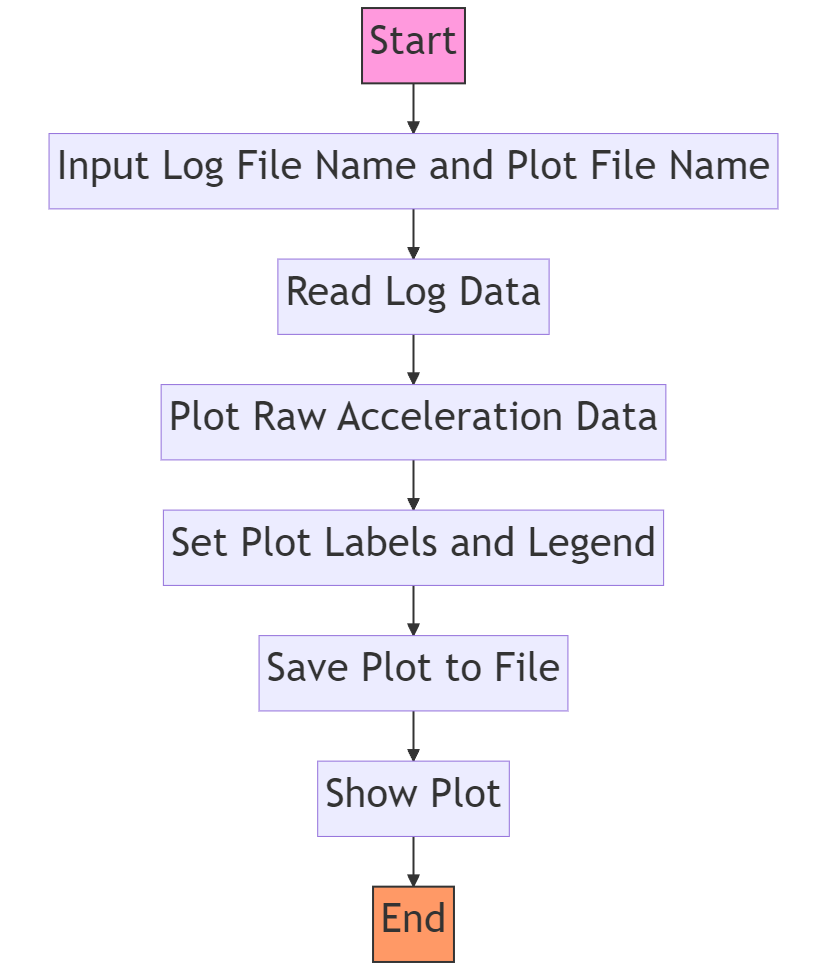
\includegraphics[width=\textwidth]{Sections/Design-Process/proto1-soft-diagram-sender-plot.png}
	\label{proto1-soft-diagram-sender-plot}
\end{figure}

\subsection{Python Receiver Plotting Script}
\begin{figure}[H]
	\centering
	\caption{Prototype 1 Software Diagram: Receiver Plotting}
	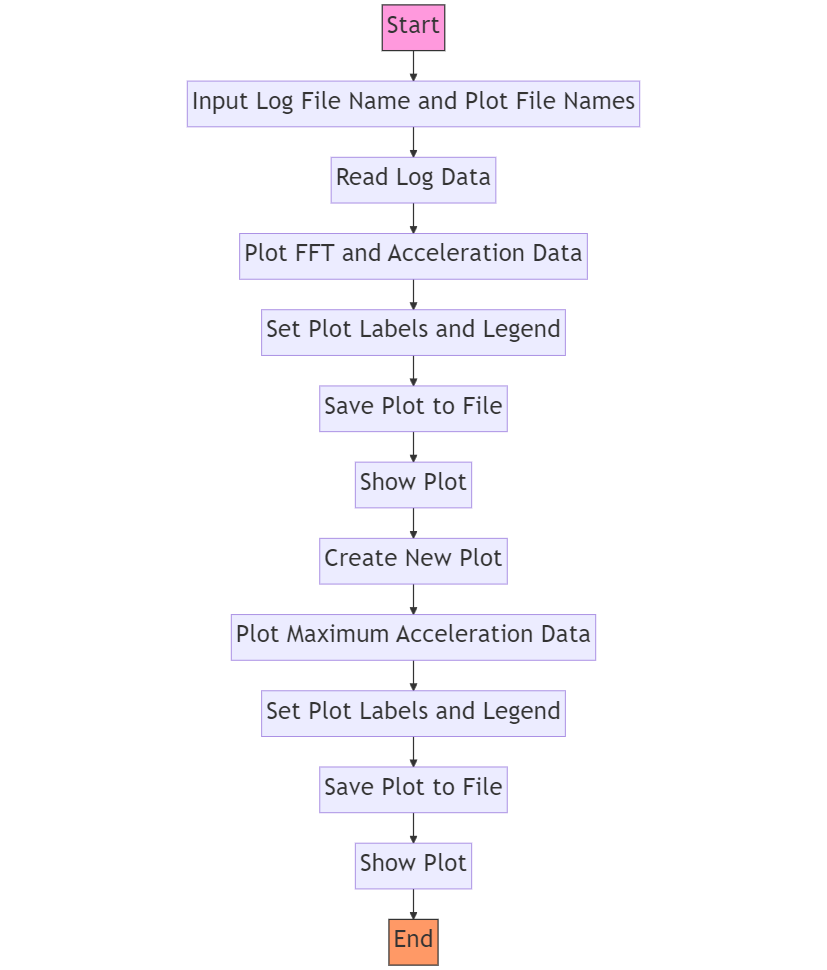
\includegraphics[width=\textwidth]{Sections/Design-Process/proto1-soft-diagram-receiver-plot.png}
	\label{proto1-soft-diagram-receiver-plot}
\end{figure}	

\clearpage
\section{Programs}
\subsection{Prototype 1: Sender Main Program}
\begin{verbatim}
#include "Sender.h"

double xZero = 0.0; double yZero = 0.0; double zZero = 0.0;

void setup() {
  // //Initialise Serial connection
  Serial.begin(9600);
  LoRa.begin(915E6);
  callibrate(256, xZero, yZero, zZero);
}

void loop() {
  // ---------- VARIABLES ----------
  // FFT SAMPLING
  double real_x_axis[sample_n]{}; double imag_x_axis[sample_n]{};
  double real_y_axis[sample_n]{}; double imag_y_axis[sample_n]{};
  double real_z_axis[sample_n]{}; double imag_z_axis[sample_n]{};
  
  // ACCELERATION SAMPLING
  double xAccel[sample_n]{}; double yAccel[sample_n]{}; 
  double zAccel[sample_n]{};

  // VELOCITY SAMPLING
  double xVel[sample_n]{}; double yVel[sample_n]{}; 
  double zVel[sample_n]{};

  // DISPLACEMENT SAMPLING
  double xDisp[sample_n]{}; double yDisp[sample_n]{}; 
  double zDisp[sample_n]{};

  // MAXIMUM ACCELERATION
  double maxAccelX = 0.0; double maxAccelY = 0.0; 
  double maxAccelZ = 0.0;

  // MAXIMUM FREQUENCY
  double xFreq = 0.0; double yFreq = 0.0; double zFreq = 0.0;
  // ---------- VARIABLES ----------

  // ---------- SAMPLE RAW DATA ----------
  readRawData(real_x_axis, real_y_axis, real_z_axis);
  // ---------- SAMPLE RAW DATA ----------
  
  // ---------- TURN RAW DATA INTO ACCELERATION (m/s/s) ----------
  processRawData(xAccel, yAccel, zAccel, real_x_axis, real_y_axis, 
                  real_z_axis, xZero, yZero, zZero);
  // ---------- TURN RAW DATA INTO ACCELERATION (m/s/s) ----------
  
  // ---------- SERIAL PRINT ACCELERATION (m/s/s) ----------
  printAxisValues(xAccel, yAccel, zAccel);
  // ---------- SERIAL PRINT ACCELERATION (m/s/s) ----------

  // ---------- FIND MAX ACCELERATION ----------
  maxAccelX = findMaxAbs(xAccel);
  maxAccelY = findMaxAbs(yAccel);
  maxAccelZ = findMaxAbs(zAccel);
  // ---------- FIND MAX ACCELERATION ----------

  // ---------- REMOVE HIGH FREQUENCIES ----------
  lowPassFilter(xAccel);
  lowPassFilter(yAccel);
  lowPassFilter(zAccel);
  // ---------- REMOVE HIGH FREQUENCIES ----------

  // ---------- COMPUTE FFT ----------
  arduinoFFT xFFT(xAccel, imag_x_axis, sample_n, sampling_rate);
  arduinoFFT yFFT(yAccel, imag_y_axis, sample_n, sampling_rate);
  arduinoFFT zFFT(zAccel, imag_z_axis, sample_n, sampling_rate);

  xFFT.DCRemoval();
  yFFT.DCRemoval();
  zFFT.DCRemoval();

  xFFT.Windowing(window_type, FFT_dir);
  yFFT.Windowing(window_type, FFT_dir);
  zFFT.Windowing(window_type, FFT_dir);

  xFFT.Compute(FFT_dir);
  yFFT.Compute(FFT_dir);
  zFFT.Compute(FFT_dir);

  xFFT.ComplexToMagnitude();
  yFFT.ComplexToMagnitude();
  zFFT.ComplexToMagnitude();
  // ---------- COMPUTE FFT ----------

  // ---------- FIND HIGHEST FREQUENCY ----------
  xFreq = xFFT.MajorPeak();
  yFreq = yFFT.MajorPeak();
  zFreq = zFFT.MajorPeak();
  // ---------- FIND HIGHEST FREQUENCY ----------

  // ---------- CONVERT NAN TO 0 ----------
  checkNan(maxAccelX); 
  checkNan(maxAccelY);
  checkNan(maxAccelZ);

  checkNan(xFreq); 
  checkNan(yFreq);
  checkNan(zFreq);
  // ---------- CONVERT NAN TO 0 ----------

 // ---------- TRANSMIT LORA PACKET ----------
  LoRa.beginPacket();
  LoRa.write((uint8_t*)&xFreq, sizeof(xFreq));
  LoRa.write((uint8_t*)&yFreq, sizeof(yFreq));  
  LoRa.write((uint8_t*)&zFreq, sizeof(zFreq));

  LoRa.write((uint8_t*)&maxAccelX, sizeof(maxAccelX));
  LoRa.write((uint8_t*)&maxAccelY, sizeof(maxAccelY));
  LoRa.write((uint8_t*)&maxAccelZ, sizeof(maxAccelZ));
  LoRa.endPacket();
  // ---------- TRANSMIT LORA PACKET ----------
}
\end{verbatim}

\clearpage
\subsection{Prototype 1: Sender Header File}
\begin{verbatim}
#ifndef Sender_h
#define Sender_h

#include "Arduino.h"
#include <algorithm>
#include <math.h>
#include <MKRWAN.h>
#include <arduinoFFT.h>
#include <LoRa.h>
#include <stdio.h>
#include <iostream> 

static constexpr double pi = 3.14159265358979323846;

//---------- Accelerometer Values ----------
static const int x_axis = A1;
static const int y_axis = A2;
static const int z_axis = A3;
static const int adc_resolution = 4096; //12 BIT ADC
static const double g = 9.81;
const double noiseThreshold = 0.15;
// CALIBRATION
// const double vRef = 3.3; //3.3V reference / supply
const double vRef = 3.0; // BATTERY CONNECTION
static const double sensitivity = 0.33; //330 mV/g at 3.3V
//---------- Accelerometer Values ----------

//---------- FFT Values ----------
static const int frequency = 2;
// THIS IS THE MAXIMUM FREQUENCY THAT THE FFT CAN DETECT
static const int maxFreq = 25; 
static const uint16_t sample_n = 128; //MUST BE EXP 2
// SAMPLING RATE MUST BE AT LEAST TWICE THE MAX FREQUENCY
static const constexpr double sampling_rate = maxFreq * 2; 
 //Gives sample interval in milliseconds
static constexpr double sample_interval = ((1.0/sampling_rate) 
                                            * 1000);

// ---------- FILTER VALUES ----------
constexpr double HP_Fc = 0.5; // high pass cut-off frequency 
constexpr double LP_Fc = 5; // low pass cut-off frequency
constexpr double sampling_period = 1.0 / sampling_rate;

constexpr double HP_alpha = (1 - (2 * pi * HP_Fc 
                                * sampling_period)) 
                            / (1 + (2 * pi * HP_Fc 
                                * sampling_period));
constexpr double LP_alpha = 1 / (1 + (2 * pi * LP_Fc 
                                * sampling_period));

const double alpha = 0.95;
// ---------- FILTER VALUES ----------

//FFT Function Values
// #define window_type FFT_WIN_TYP_HAMMING
#define window_type FFT_WIN_TYP_HANN
#define FFT_dir FFT_FORWARD
//---------- FFT Values ----------

// ---------- FUNCTIONS ----------
double findMaxAbs(const double data[]);
void lowPassFilter(double *data);
void highPassFilter(double *data);
void addGravity(double arr[]);
int findMaxIndex(double arr[]);
double findAvg(double arr[]);
void removeBias(double arr[]);
void integrate(const double arr[], double dt, double integrated[]);
void readRawData(double real_x_axis[], double real_y_axis[], 
                 double real_z_axis[]);
void processRawData(double xAccel[], double yAccel[], 
                    double zAccel[], 
                    const double real_x_axis[], 
                    const double real_y_axis[], 
                    const double real_z_axis[], double xZero, 
                    double yZero, 
                    double zZero);
void integrate(const double xIn[], const double yIn[], 
                const double zIn[], double xOut[], 
                double yOut[], double zOut[]);
// ---------- FUNCTIONS ----------

// ---------- TEST FUNCTIONS ----------
void genSineWave(double arr[]);
void genZeroWave(double arr[]);
void printAxisValues(double xAccel[], double yAccel[], 
                        double zAccel[]);
void printAxisVal(double xFreq, double yFreq, double zFreq);
void printAxisValueSingle(double accel[]);
void callibrate(int callibration_samples, double& xZero, 
                double& yZero, double& zZero);
void checkNan(double& freq);
// ---------- TEST FUNCTIONS ----------

#endif
\end{verbatim}

\subsection{Prototype 1: Sender Functions}

\begin{verbatim}
#include "Sender.h"

void callibrate (int callibration_samples, double& xZero,
                 double& yZero, double& zZero) {
    Serial.println("Calibrating Accelerometer...");

    double offsetX = 0;
    double offsetY = 0;
    double offsetZ = 0;

    for (int i = 0; i < callibration_samples; i++) {
        double rawX = analogRead(x_axis);
        double rawY = analogRead(y_axis);
        double rawZ = analogRead(z_axis);

        double voltageX = (rawX * vRef) / (adc_resolution - 1);
        double voltageY = (rawY * vRef) / (adc_resolution - 1);
        double voltageZ = (rawZ * vRef) / (adc_resolution - 1);

        double accelerationX = (voltageX - vRef / 2) / sensitivity;
        double accelerationY = (voltageY - vRef / 2) / sensitivity;
        double accelerationZ = (voltageZ - vRef / 2) / sensitivity - 1;

        offsetX += accelerationX;
        offsetY += accelerationY;
        offsetZ += accelerationZ;
        delay(10);
    }

    offsetX /= callibration_samples;
    offsetY /= callibration_samples;
    offsetZ /= callibration_samples;

    // ---------- MUST BE TURNED OFF IF PWR IS BATTERY ----------
    // Serial.print("Offset X: ");
    // Serial.println(offsetX, 6);
    // Serial.print("Offset Y: ");
    // Serial.println(offsetY, 6);
    // Serial.print("Offset ccoffsetZ: ");
    // Serial.println(offsetZ, 6);
    // ---------- MUST BE TURNED OFF IF PWR IS BATTERY ----------

    xZero = offsetX;
    yZero = offsetY;
    zZero = offsetZ;
}

double findMaxAbs(const double data[]) {
  double maxVal = 0;
  for (int i = 0; i < sample_n; ++i) {
    double absVal = abs(data[i]);
    if (absVal > maxVal) {
      maxVal = absVal;
    }
  }
  return maxVal;
}

double findMax(const float data[]) {
  double maxVal = 0;
  for (int i = 0; i < sample_n; ++i) {
    double absVal = data[i];
    if (absVal > maxVal) {
      maxVal = absVal;
    }
  }
  return maxVal;
}

void lowPassFilter(double *data) {
  // Initialize with the first value of the data array
  double filteredData = data[0];

  for (uint16_t i = 1; i < sample_n; i++) {
    filteredData = LP_alpha * data[i] + (1.0 - LP_alpha) 
                    * filteredData;
    data[i] = filteredData;
  }
}

double findAvg(double arr[]) {
  double sum = 0.0;
  for (int i = 0; i < sample_n; i++) {
    sum += arr[i];
  }
  return sum / sample_n;
}

void removeBias(double arr[]) { 
  double bias = findAvg(arr);
  for (int i = 0; i < sample_n; i++) {
    arr[i] -= bias;
  }
}

void readRawData(double real_x_axis[], double real_y_axis[], 
                  double real_z_axis[]) {
  for (int i = 0; i < sample_n; i++) {
    // READ RAW DATA FROM ANALOG PINS
    real_x_axis[i] = analogRead(x_axis);
    real_y_axis[i] = analogRead(y_axis);
    real_z_axis[i] = analogRead(z_axis);
    // SAMPLING INTERVAL
    delay(sample_interval);
  }
}

void processRawData(double xAccel[], double yAccel[], 
                    double zAccel[], const double real_x_axis[], 
                    const double real_y_axis[], 
                    const double real_z_axis[], 
                    double xZero, double yZero, double zZero) {
  for (int i = 0; i < sample_n; i++) {
    // CONVERT ADC LEVEL TO A VOLTAGE
    double voltageX = ((real_x_axis[i] * vRef) / (adc_resolution - 1));
    double voltageY = ((real_y_axis[i] * vRef) / (adc_resolution - 1));
    double voltageZ = ((real_z_axis[i] * vRef) / (adc_resolution - 1));

    xAccel[i] = ((voltageX - vRef / 2) / sensitivity - xZero) * g;
    yAccel[i] = ((voltageY - vRef / 2) / sensitivity - yZero) * g;
    // Subtract gravity
    zAccel[i] = ((voltageZ - vRef / 2) / sensitivity - zZero - 1) * g; 

    // // Apply threshold to remove noise
    xAccel[i] = (abs(xAccel[i]) <= 0.7) ? 0 : xAccel[i];
    yAccel[i] = (abs(yAccel[i]) <= 0.9) ? 0 : yAccel[i];
    zAccel[i] = (abs(zAccel[i]) <= 0.1) ? 0 : zAccel[i];
  }
}

void checkNan(float& freq) {
 if (isnan(freq)) {
  freq = 0;
 }
}
\end{verbatim}

\subsection{Prototype 1: Recevier Main Program}
\begin{verbatim}
#include "Receiver.h"

void setup() {
  //Initialise Serial connection
  Serial.begin(9600);
  //Initialise LoRa Connection
  if (!LoRa.begin(915E6)) {
    Serial.println("Starting LoRa failed!");
    while (1);
  }
  Serial.println("LoRa Modem Started");
}

void loop() {
    if (LoRa.parsePacket()) {
    float receivedFreqX;
    float receivedFreqY;
    float receivedFreqZ;

    float receviedAccelX;
    float receviedAccelY;
    float receviedAccelZ;

    LoRa.readBytes((uint8_t*)&receivedFreqX, sizeof(receivedFreqX));
    LoRa.readBytes((uint8_t*)&receivedFreqY, sizeof(receivedFreqY));
    LoRa.readBytes((uint8_t*)&receivedFreqZ, sizeof(receivedFreqZ));

    LoRa.readBytes((uint8_t*)&receviedAccelX, sizeof(receviedAccelX));
    LoRa.readBytes((uint8_t*)&receviedAccelY, sizeof(receviedAccelY));
    LoRa.readBytes((uint8_t*)&receviedAccelZ, sizeof(receviedAccelZ));

    Serial.print(receivedFreqX); 
    Serial.print(" ");
    Serial.print(receivedFreqY);
    Serial.print(" ");
    Serial.print(receivedFreqZ);       

    Serial.print(" ");
    Serial.print(receviedAccelX); 
    Serial.print(" ");
    Serial.print(receviedAccelY);
    Serial.print(" ");
    Serial.println(receviedAccelZ);
  }
}
\end{verbatim}

\subsection{Prototype 1: Sender Logger Program}
\begin{verbatim}
import matplotlib.pyplot as plt
import serial
import time
import os

# MAC ADDRESS
# PORT = '/dev/tty.usbmodem1413301'
# PC ADDERSS
PORT = 'COM3'
BAUD_RATE = 9600
ser = serial.Serial(PORT, BAUD_RATE, timeout=1)

raw_xAccel = []
raw_yAccel = []
raw_zAccel = [] 

fname = input("Enter the name of the log file: ")

def read_serial_data():
    data = ser.readline().decode('utf-8').strip()
    if data:
        variables = data.split(' ')
        if len(variables) == 3 and all(variables):
            try:
                var1, var2, var3 = map(float, variables)
                return var1, var2, var3
            except ValueError:
                print("ERROR: INVALID DATA RECEIVED")
    return None, None, None

print("Ctrl-C to stop logging")

try:
    while True:
        var1, var2, var3 = read_serial_data()
        if var1 is not None and var2 is not None and var3 is not None:
            raw_xAccel.append(var1) 
            raw_yAccel.append(var2)
            raw_zAccel.append(var3)
        time.sleep(0.01)

except KeyboardInterrupt:
    print("Interrupted by user.")

finally:
    # Close the serial port
    ser.close()
    print("Serial port closed.")

# Open and overwrite senderlog
dir_path = "serialPlot/logs/"
full_path = os.path.join(dir_path, fname)

f = open(full_path, "w")
for i in range(len(raw_xAccel)):
    f.writelines([str(raw_xAccel[i]), " ", str(raw_yAccel[i]), \
                    " ", str(raw_zAccel[i]), "\n"])
\end{verbatim}
\subsection{Prototype 1: Sender Plotter Program}
\begin{verbatim}
import matplotlib.pyplot as plt
import time
import os

plt.close('all')

def read_log_data():
    raw_xAccel = []
    raw_yAccel = []
    raw_zAccel = []

    with open(full_path, "r") as f:
        for line in f:
            var1, var2, var3 = map(float, line.split())
            raw_xAccel.append(var1)
            raw_yAccel.append(var2)
            raw_zAccel.append(var3)
    return raw_xAccel, raw_yAccel, raw_zAccel

fname = input("Enter the name of the log file: ")
fname2 = input("Enter the name of the raw acceleration \
               plot file (with file extension): ")

dir_path = "serialPlot/logs/"
full_path = os.path.join(dir_path, fname)

dir_path2 = "serialPlot/plots/"
full_path2 = os.path.join(dir_path2, fname2)

raw_xAccel, raw_yAccel, raw_zAccel = read_log_data()

# Create the plot
plt.plot(raw_xAccel, label="x_axis")
plt.plot(raw_yAccel, label="y_axis")
plt.plot(raw_zAccel, label="z_axis")

# Set plot labels and legend
plt.title("Raw Acceleration")
plt.xlabel("Samples")
plt.ylabel("Acceleration (m/s/s)")
plt.legend()

# Save the figure as a high-resolution PNG file
plt.savefig(full_path2, dpi=300)

# Display the plot
plt.show()
\end{verbatim}
\subsection{Prototype 1: Receiver Logger Program}
\begin{verbatim}
import matplotlib.pyplot as plt
import serial
import time
import os

# MAC ADDRESS
# PORT = '/dev/tty.usbmodem141401'
# PC ADDERSS
PORT = 'COM5'
BAUD_RATE = 9600
ser = serial.Serial(PORT, BAUD_RATE, timeout=1)

xFreq = []
yFreq = []
zFreq = [] 

xAccel = []
yAccel = []
zAccel = []

fname = input("Enter the name of the log file: ")

def read_serial_data():
    data = ser.readline().decode('utf-8').strip()
    if data:
        variables = data.split(' ')
        if len(variables) == 6 and all(variables):
            try:
                var1, var2, var3, var4, var5, var6 = map(float, variables)
                return var1, var2, var3, var4, var5, var6
            except ValueError:
                print("ERROR: INVALID DATA RECEIVED")
    return None, None, None, None, None, None

print("Ctrl-C to stop logging")

try:
    while True:
        var1, var2, var3, var4, var5, var6 = read_serial_data()
        if var1 is not None and var2 is not None and var3 is not None\
            and var4 is not None and var5 is not None and var6 is not None:
            xFreq.append(var1) 
            yFreq.append(var2)
            zFreq.append(var3)

            xAccel.append(var4)
            yAccel.append(var5)
            zAccel.append(var6)
        time.sleep(0.01)

except KeyboardInterrupt:
    print("Interrupted by user.")

finally:
    # Close the serial port
    ser.close()
    print("Serial port closed.")

# Open and overwrite senderlog
dir_path = "serialPlot/logs/"
full_path = os.path.join(dir_path, fname)

f = open(full_path, "w")
for i in range(len(xFreq)):
    f.writelines([str(xFreq[i]), " ", str(yFreq[i]), " ", str(zFreq[i]), \
                  " ", str(xAccel[i]), " ", str(yAccel[i]), \
                    " ", str(zAccel[i]), "\n"]) 
\end{verbatim}
\subsection{Prototype 1: Receiver Plotter Program}
\begin{verbatim}
import matplotlib.pyplot as plt
import serial
import time
import os

plt.close('all')

def read_log_data():
    xVar = []
    yVar = []
    zVar = [] 

    xAccel = []
    yAccel = []
    zAccel = []

    with open(full_path, "r") as f:
        for line in f:
            var1, var2, var3, var4, var5, var6 = map(float, line.split())
            xVar.append(var1)
            yVar.append(var2)
            zVar.append(var3)

            xAccel.append(var4)
            yAccel.append(var5)
            zAccel.append(var6)

    return xVar, yVar, zVar, xAccel, yAccel, zAccel

# Open and overwrite senderlog
fname = input("Enter the name of the log file: ")
fname2 = input("Enter the name of the FFT plot file \
               (with file extension): ")
fname3 = input("Enter the name of the accleration \
               plot file (with file extension): ")

dir_path = "serialPlot/logs/"
full_path = os.path.join(dir_path, fname)

dir_path2 = "serialPlot/plots/"
full_path2 = os.path.join(dir_path2, fname2)

dir_path3 = "serialPlot/plots/"
full_path3 = os.path.join(dir_path3, fname3)

xVar, yVar, zVar, xAccel, yAccel, zAccel = read_log_data()

print("Plotting FFT and Maximum Acceleration")

# Create the plot
plt.plot(xVar, label="x_axis")
plt.plot(yVar, label="y_axis")
plt.plot(zVar, label="z_axis")

# Set plot labels and legend
plt.title("FFT")
plt.xlabel("N's")
plt.ylabel("Frequency (Hz)")
plt.legend()

# Save the figure as a high-resolution PNG file
plt.savefig(full_path2, dpi=300)

# Display the plot
plt.show()

plt.figure()  # Create a new figure for the second plot
plt.plot(xAccel, label="x_axis")
plt.plot(yAccel, label="y_axis")
plt.plot(zAccel, label="z_axis")

# Set plot labels and legend
plt.title("Maximum Acceleration")
plt.xlabel("N's")
plt.ylabel("Max Acceleration (m/s/s)")
plt.legend()

# Save the second figure as a high-resolution PNG files
plt.savefig(full_path3, dpi=300)

# Display the second plot
plt.show()
\end{verbatim}
\subsection{Prototype 2: Sender Main Program}
\begin{verbatim}
#include "arduino_secrets.h"

#include "thingProperties.h"
#include "Sender.h"

double xZero = 0.0; double yZero = 0.0; double zZero = 0.0;
//Store total max values for averaging later
float totalMaxAccelX = 0.0; float totalMaxAccelY = 0.0; 
float totalMaxAccelZ = 0.0;
float totalMaxFreqX = 0.0; float totalMaxFreqY = 0.0; 
float totalMaxFreqZ = 0.0;
//Record the number of computations within the time limit
int computationCount = 0;
//Timing variables
unsigned long previousMillis = 0;
const long interval = 60000; //test scenario 60 seconds

void setup() {
  // Initialize serial and wait for port to open:
  Serial.begin(9600);
  // This delay gives the chance to wait for a Serial Monitor 
  //without blocking if none is found
  delay(1500);

  // Defined in thingProperties.h
  initProperties();

  // Connect to Arduino IoT Cloud
  ArduinoCloud.begin(ArduinoIoTPreferredConnection);
  
  setDebugMessageLevel(2);
  ArduinoCloud.printDebugInfo();
  delay(1500);
  
  callibrate(256, xZero, yZero, zZero);
  delay(1500);
}

void loop() {
  ArduinoCloud.update();

  // ---------- VARIABLES ----------
  double real_x_axis[sample_n] {}; 
  double imag_x_axis[sample_n] {};
  double real_y_axis[sample_n] {}; 
  double imag_y_axis[sample_n] {};
  double real_z_axis[sample_n] {}; 
  double imag_z_axis[sample_n] {};

  // ACCELERATION SAMPLING
  double xAccel[sample_n] {}; double yAccel[sample_n] {}; 
  double zAccel[sample_n] {};

  // MAXIMUM ACCELERATION
  float maxAccelX = 0.0; float maxAccelY = 0.0; 
  float maxAccelZ = 0.0;

  // MAXIMUM FREQUENCY
  float xFreq = 0.0; float yFreq = 0.0; float zFreq = 0.0;
  // ---------- VARIABLES ----------

  // ---------- SAMPLE RAW DATA ----------
  readRawData(real_x_axis, real_y_axis, real_z_axis);
  // ---------- SAMPLE RAW DATA ----------

  // ---------- TURN RAW DATA INTO ACCELERATION (m/s/s) ----------
  processRawData(xAccel, yAccel, zAccel, real_x_axis,
                  real_y_axis, real_z_axis,
                  xZero, yZero, zZero);
  // ---------- TURN RAW DATA INTO ACCELERATION (m/s/s) ----------

  // ---------- SERIAL PRINT ACCELERATION (m/s/s) ----------
  // printAxisValues(xAccel, yAccel, zAccel);
  // ---------- SERIAL PRINT ACCELERATION (m/s/s) ----------

  // ---------- FIND MAX ACCELERATION ----------
  maxAccelX = float(findMaxAbs(xAccel));
  maxAccelY = float(findMaxAbs(yAccel));
  maxAccelZ = float(findMaxAbs(zAccel));
  // ---------- FIND MAX ACCELERATION ----------

  // ---------- REMOVE HIGH FREQUENCIES ----------
  lowPassFilter(xAccel);
  lowPassFilter(yAccel);
  lowPassFilter(zAccel);
  // ---------- REMOVE HIGH FREQUENCIES ----------

  // ---------- COMPUTE FFT ----------
  arduinoFFT xFFT(xAccel, imag_x_axis, sample_n, sampling_rate);
  arduinoFFT yFFT(yAccel, imag_y_axis, sample_n, sampling_rate);
  arduinoFFT zFFT(zAccel, imag_z_axis, sample_n, sampling_rate);

  xFFT.DCRemoval();
  yFFT.DCRemoval();
  zFFT.DCRemoval();

  xFFT.Windowing(window_type, FFT_dir);
  yFFT.Windowing(window_type, FFT_dir);
  zFFT.Windowing(window_type, FFT_dir);

  xFFT.Compute(FFT_dir);
  yFFT.Compute(FFT_dir);
  zFFT.Compute(FFT_dir);

  xFFT.ComplexToMagnitude();
  yFFT.ComplexToMagnitude();
  zFFT.ComplexToMagnitude();
  // ---------- COMPUTE FFT ----------

  // ---------- FIND HIGHEST FREQUENCY ----------
  xFreq = float(xFFT.MajorPeak());
  yFreq = float(yFFT.MajorPeak());
  zFreq = float(zFFT.MajorPeak());
  // ---------- FIND HIGHEST FREQUENCY ----------

  // ---------- CONVERT NAN TO 0 ----------
  checkNan(maxAccelX);
  checkNan(maxAccelY);
  checkNan(maxAccelZ);

  checkNan(xFreq);
  checkNan(yFreq);
  checkNan(zFreq);
  // ---------- CONVERT NAN TO 0 ----------

  totalMaxAccelX += maxAccelX;
  totalMaxAccelY += maxAccelY;
  totalMaxAccelZ += maxAccelZ;

  totalMaxFreqX += xFreq;
  totalMaxFreqY += yFreq;
  totalMaxFreqZ += zFreq;

  computationCount++;

  unsigned long currentMillis = millis();
  if (currentMillis - previousMillis >= interval) {
    previousMillis = currentMillis;

    float averageMaxAccelX = totalMaxAccelX / computationCount;
    float averageMaxAccelY = totalMaxAccelY / computationCount;
    float averageMaxAccelZ = totalMaxAccelZ / computationCount;

    float averageMaxFreqX = totalMaxFreqX / computationCount;
    float averageMaxFreqY = totalMaxFreqY / computationCount;
    float averageMaxFreqZ = totalMaxFreqZ / computationCount;

    Serial.print(averageMaxAccelX);
    Serial.print(" ");
    Serial.print(averageMaxAccelY);
    Serial.print(" ");
    Serial.print(averageMaxAccelZ);
    Serial.print(" ");
    Serial.print(averageMaxFreqX);
    Serial.print(" ");
    Serial.print(averageMaxFreqY);
    Serial.print(" ");
    Serial.println(averageMaxFreqZ);

    dev1_cloud_avg_max_accel_x = averageMaxAccelX;
    dev1_cloud_avg_max_accel_y = averageMaxAccelY;
    dev1_cloud_avg_max_accel_z = averageMaxAccelZ;

    dev1_cloud_avg_max_freq_x = averageMaxFreqX;
    dev1_cloud_avg_max_freq_y = averageMaxFreqY;
    dev1_cloud_avg_max_freq_z = averageMaxFreqZ;

    totalMaxAccelX = 0.0;
    totalMaxAccelY = 0.0;
    totalMaxAccelZ = 0.0;

    totalMaxFreqX = 0.0;
    totalMaxFreqY = 0.0;
    totalMaxFreqZ = 0.0;

    computationCount = 0;
  }
}
\end{verbatim}
\subsection{Prototype 2: Sender Thing Properties Header File}
\begin{verbatim}
// Code generated by Arduino IoT Cloud, DO NOT EDIT.

#include <ArduinoIoTCloud.h>
#include <Arduino_ConnectionHandler.h>


const char THING_ID[] = "09f4b4cd-c539-49df-9701-d4c915b536ae";

const char APPEUI[]   = SECRET_APP_EUI;
const char APPKEY[]   = SECRET_APP_KEY;


float dev1_cloud_avg_max_accel_x;
float dev1_cloud_avg_max_accel_y;
float dev1_cloud_avg_max_accel_z;
float dev1_cloud_avg_max_freq_x;
float dev1_cloud_avg_max_freq_y;
float dev1_cloud_avg_max_freq_z;

void initProperties(){
  ArduinoCloud.setThingId(THING_ID);
  ArduinoCloud.addProperty(dev1_cloud_avg_max_accel_x, 1,
                            READ, ON_CHANGE, NULL);
  ArduinoCloud.addProperty(dev1_cloud_avg_max_accel_y, 2,
                            READ, ON_CHANGE, NULL);
  ArduinoCloud.addProperty(dev1_cloud_avg_max_accel_z, 4,
                            READ, ON_CHANGE, NULL);
  ArduinoCloud.addProperty(dev1_cloud_avg_max_freq_x, 5, 
                            READ, ON_CHANGE, NULL);
  ArduinoCloud.addProperty(dev1_cloud_avg_max_freq_y, 7, 
                            READ, ON_CHANGE, NULL);
  ArduinoCloud.addProperty(dev1_cloud_avg_max_freq_z, 8, 
                            READ, ON_CHANGE, NULL);

}

LoRaConnectionHandler ArduinoIoTPreferredConnection(APPEUI,  
      APPKEY, _lora_band::AU915, "ff000001f000ffff00020000");
\end{verbatim}

\section{Network Layer}
\subsection{TNN Live Data}
\begin{figure}[H]
	\centering
	\caption{TNN Live Data View}
	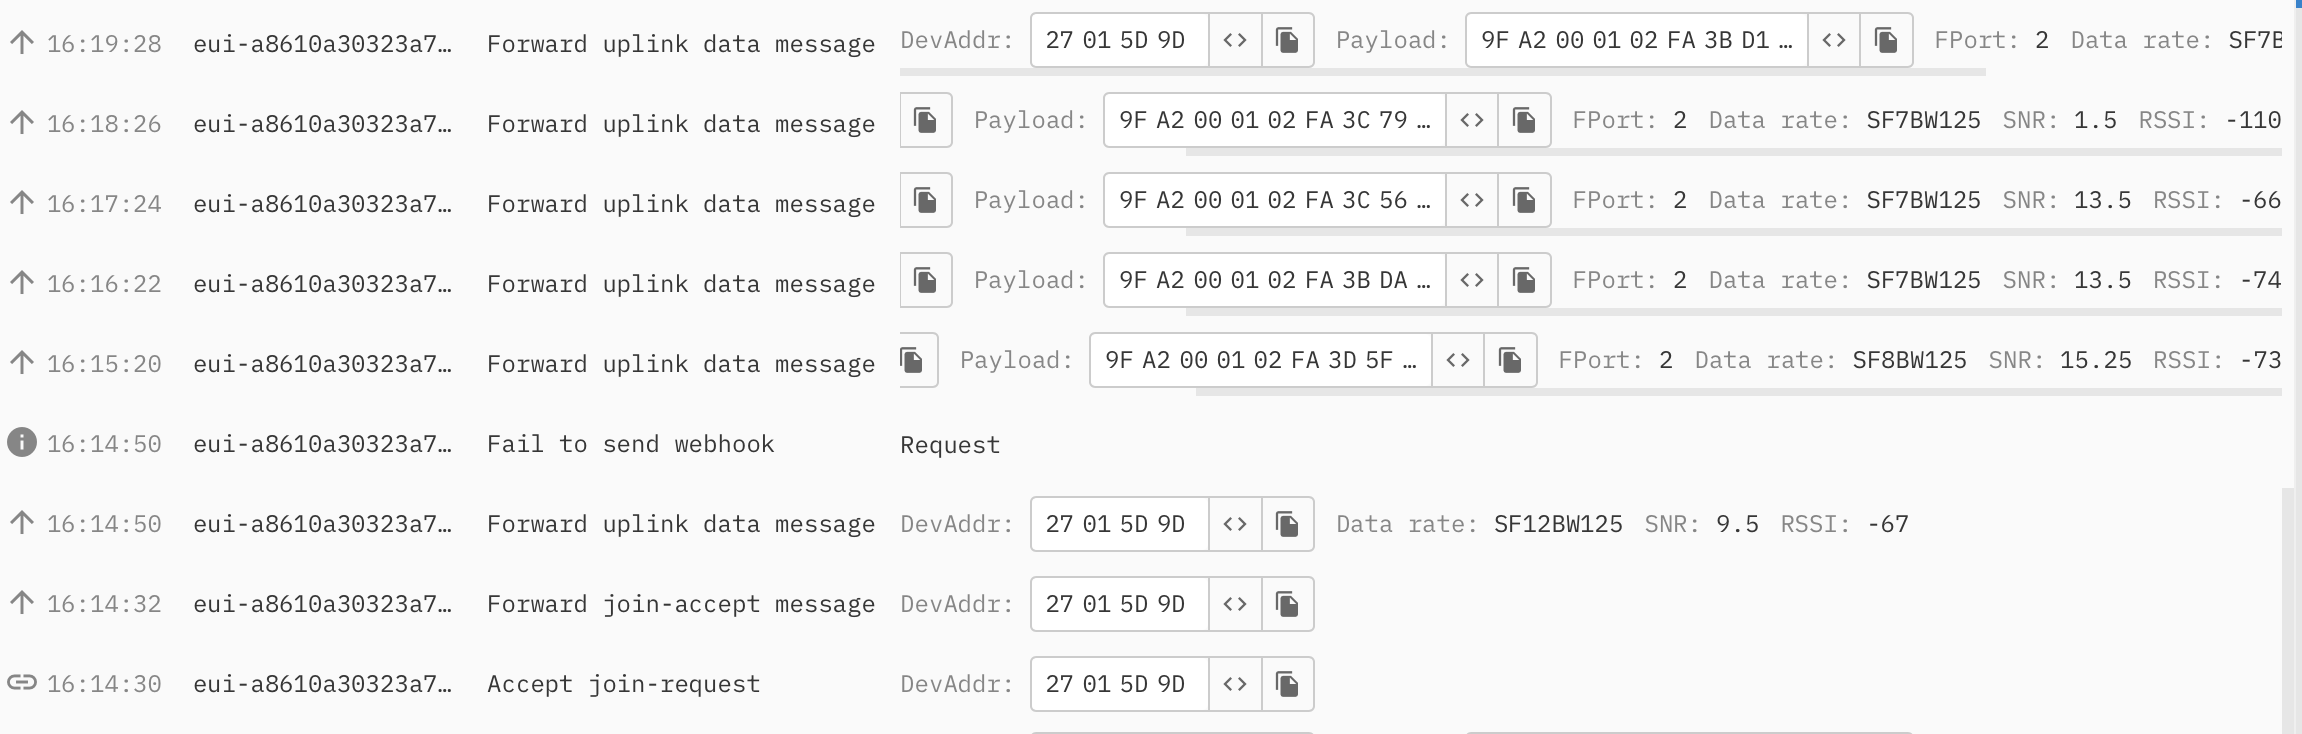
\includegraphics[width=\textwidth]{Sections/Appendix/TNN-live.png}
	\label{tnn-live}
\end{figure}

\subsection{Arduino Iot Cloud Dashboard}
\begin{figure}[H]
	\centering
	\caption{Arduino IoT Cloud Dashboard Desktop View}
	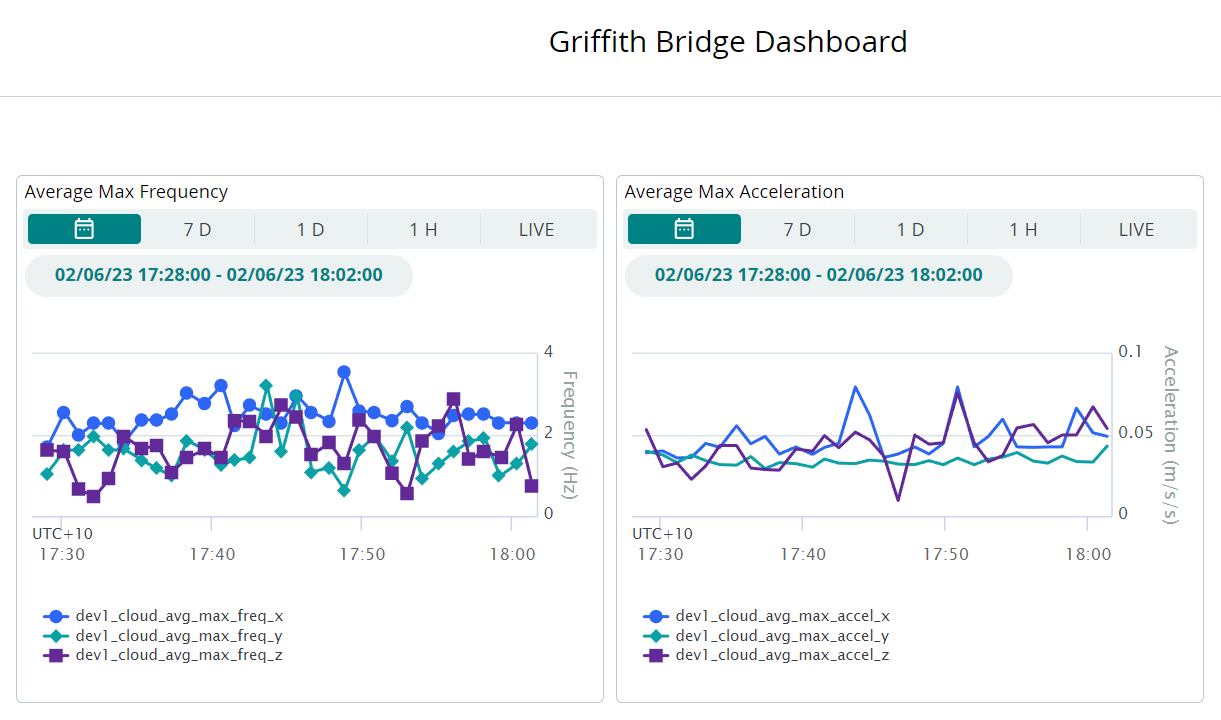
\includegraphics[width=\textwidth]{Sections/Appendix/dashboard.png}
	\label{dashboard}
\end{figure}

\begin{figure}[H]
	\centering
	\caption{Arduino IoT Cloud Dashboard Phone View}
	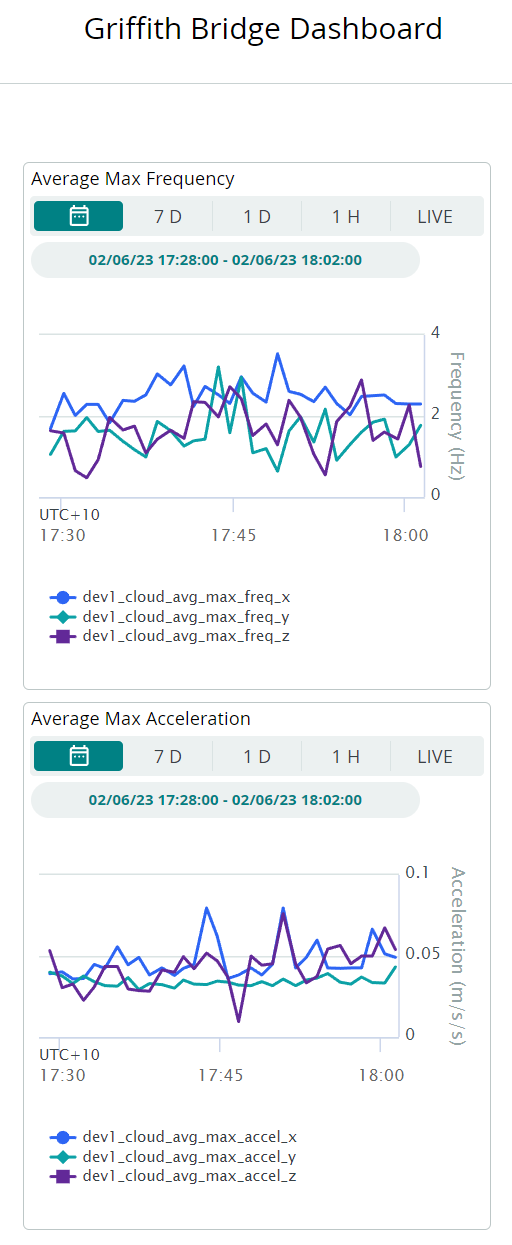
\includegraphics[scale=0.6]{Sections/Appendix/dashboard-phone.png}
	\label{dashboard-phone}
\end{figure}



\end{document}